\ifdefined\fullversion
\else
\def\fullversion{1}    % 0 = conference version; 1 = full version
\fi

\ifdefined\cameraversion
\else
\def\cameraversion{0}    % 0 = long version; 1 = proceedings version
\fi
\def\showoverflow{1}   % 1 = show overflows
\def\allow{1}      % 0 = remove todo command
\def\anonymous{1}      % 1 = anonymous

% \documentclass[envcountsame,runningheads,notitlepage]{llncs}
\documentclass[envcountsame,runningheads,notitlepage]{llncs}
\ifnum\fullversion=1
\usepackage[a4paper, margin=1.1in]{geometry}
\setlength{\marginparwidth}{2.5cm}
\fi

\usepackage{makecell}
\usepackage{amsmath} 
% \usepackage{amsthm} don't use this, makes errors
% \usepackage{wasysym} don't use this, makes errors
\usepackage[utf8]{inputenc}
\usepackage[T1]{fontenc}
% \usepackage{hyperref}
\usepackage{verbatim}
\usepackage{tikz}
\usetikzlibrary{positioning,calc}
\usepackage{xspace}
\usepackage{amssymb}
\usepackage{mathtools}
\usepackage{pifont}
\usepackage{etoolbox}
% \usepackage[normalem]{ulem}
\usepackage{booktabs}
\usepackage{bookmark}
% \usepackage[bookmarks=true]{hyperref} 
\usepackage{float} %to force my protocol environment to stay where it is

\usepackage{array}
\usepackage[capitalise,noabbrev]{cleveref}
\usepackage{cite}
\usepackage{multibib}
\usepackage{url}
\usepackage{algorithm}
% \usepackage{algpseudocode}
\usepackage{paralist}
\usepackage{mathrsfs}
\usepackage{relsize}
\usepackage{stmaryrd}
\usepackage[textsize=small]{todonotes}
\usepackage{multirow}
% \usepackage[lambda,n,operators]{cryptocode}
% \usepackage{caption} % Removed to avoid warning with llncs class
\usepackage[skip=10pt plus1pt, indent=40pt]{parskip}
\usepackage{cancel} 
\usepackage[
n,
advantage,
operators,
sets,
adversary,
landau,
probability,
notions,
logic,
ff,
mm,
primitives,
events,
complexity,
oracles,
asymptotics,
keys
]{cryptocode}
\createpseudocodeblock{pcb}{center,boxed}{}{}{}

\newtoggle{notes}
\toggletrue{notes} % set to false to remove colored notes from the paper


%--------------------------------------------------------
% Custom - commitment and PS sigs
%--------------------------------------------------------
\newcommand{\BG}{\mathsf{BG}}
\newcommand{\BGGen}{\mathsf{BGGen}}
\newcommand{\Setup}{\mathsf{Setup}}
\newcommand{\OrgKeyGen}{\mathsf{OrgKeyGen}}
\newcommand{\UserKeyGen}{\mathsf{UserKeyGen}}
\newcommand{\Obtain}{\mathsf{Obtain}}
\newcommand{\Issue}{\mathsf{Issue}}
\newcommand{\MIMCABC}{\ensuremath{\mathsf{MIMC\text{-}ABC}}\xspace}
\newcommand{\UNF}{\ensuremath{\mathsf{UNF}}\xspace}
\newcommand{\UNFONE}{\ensuremath{\mathsf{UNF\text{-}1}}\xspace}
\newcommand{\UNFTWO}{\ensuremath{\mathsf{UNF\text{-}2}}\xspace}


\newcommand{\Nul}{\mathsf{N}}
\newcommand{\nul}{\mathsf{N}}
\renewcommand{\exp}{\mathsf{exp}}
\newcommand{\n}{\mathsf{n}}
\newcommand{\ABC}{\mathsf{ABC}}



\newcommand{\acu}{\mathsf{ACU}}
\newcommand{\acusetup}{\mathsf{ACU.Setup}}
\newcommand{\acuadd}{\mathsf{ACU.Add}}
\newcommand{\acudel}{\mathsf{ACU.Del}}
\newcommand{\acuvermem}{\mathsf{ACU.VerMem}}
\newcommand{\acuvernonmem}{\mathsf{ACU.VerNonMem}}


\newcommand{\rev}{\mathsf{REV}}
\newcommand{\revsetup}{\mathsf{REV.Setup}}
\newcommand{\revrevoke}{\mathsf{REV.Revoke}}
\newcommand{\revtokengen}{\mathsf{REV.TokenGen}}
\newcommand{\revtokenver}{\mathsf{REV.TokenVer}}

\newcommand{\rt}{\mathsf{rt}}

% \newcommand{\tilcm}{\tilde{\mathsf{cm}}}
\newcommand{\tilcm}{\tilde{cm}}


\renewcommand{\k}{\mathsf{k}}
\newcommand{\mb}{\textbf{m}}
\newcommand{\gb}{\textbf{g}}
\newcommand{\tilgb}{\tilde{\textbf{g}}}
\newcommand{\yb}{\textbf{y}}
\newcommand{\rd}{\Delta_r}
\newcommand{\td}{\Delta_t}
\newcommand{\ud}{\Delta_u}


%--------------------------------------------------------
% Custom - Syntax
%--------------------------------------------------------

\renewcommand{\st}{\mathsf{st}}
\newcommand{\zkx}{\mathsf{x}}
\newcommand{\zkw}{\mathsf{w}}
\newcommand{\m}{\textbf{m}}
\newcommand{\Rr}{\mathcal{R}}
\newcommand{\Lr}{\mathcal{L}}
\newcommand{\commitment}{\mathsf{Com}}
\newcommand{\secret}{\mathsf{s}}
\newcommand{\sn}{\mathsf{sn}}
\newcommand{\pid}{\mathsf{pid}}
\newcommand{\ccm}{\mathsf{ccm}}
\newcommand{\rcm}{\mathsf{rcm}}
\newcommand{\vcm}{\mathsf{vcm}}
\newcommand{\vrf}{\mathsf{vrf}}
\newcommand{\rcd}{\mathsf{rcd}}
\newcommand{\prnid}{\mathsf{prnid}}
\newcommand{\PRF}{\mathsf{PRF}}
\newcommand{\RL}{\mathcal{RL}}
\newcommand{\CL}{\mathcal{CL}}
\newcommand{\UL}{\mathcal{UL}}



\newcommand{\User}{\mathcal{U}}
\newcommand{\MCO}{\mathcal{M}}
\newcommand{\CCO}{\mathcal{C}}
\newcommand{\Auditor}{\mathcal{A}}
\newcommand{\Revoker}{\mathcal{R}}


\newenvironment{experiment}[1][]{\begin{trivlist}\item[\hskip \labelsep{\bfseries Experiment #1}]}{\end{trivlist}}


%--------------------------------------------------------
% Protocol Environment
%--------------------------------------------------------
\usepackage[utf8]{inputenc}
\usepackage{amsmath, amssymb, xcolor, enumitem, mdframed}
\usepackage[most]{tcolorbox}


\usepackage{etoolbox}
\makeatletter
\let\llncs@addcontentsline\addcontentsline
\patchcmd{\maketitle}{\addcontentsline}{\llncs@addcontentsline}{}{}
\patchcmd{\maketitle}{\addcontentsline}{\llncs@addcontentsline}{}{}
\patchcmd{\maketitle}{\addcontentsline}{\llncs@addcontentsline}{}{}
\setcounter{tocdepth}{2}
\makeatother
\usepackage{hyperref}
\usepackage{bookmark}







\makeatletter
% First, clear the current definitions
% \let\proposition\relax
% \let\endproposition\relax
% \let\lemma\relax
% \let\endlemma\relax
% \let\definition\relax
% \let\enddefinition\relax

% % Now create fresh counters
% \newcounter{proposition}
% \newcounter{lemma}
% \newcounter{definition}

% Define the environments with their own counters
% \spnewtheorem{proposition}{Proposition}{\bfseries}{\itshape}
% \spnewtheorem{lemma}{Lemma}{\bfseries}{\itshape}
% \spnewtheorem{definition}{Definition}{\bfseries}{\itshape}
% \makeatother

% \makeatletter
% \@removefromreset{proposition}{theorem}
% \@removefromreset{lemma}{theorem}
% \makeatother

\newtcbtheorem[auto counter]{protocol}{Protocol}{
    colback=white,
    colframe=black,
    fonttitle=\bfseries,
    coltitle=black,
    attach boxed title to top center={yshift=-3mm},
    boxed title style={
        colframe=black,
        colback=white,
        boxrule=0.5mm,
    },
    enhanced,
    sharp corners,
    % Add internal padding
    top=8pt,
    bottom=8pt,
    left=12pt,
    right=12pt,
      break at=none,
    % Add spacing between paragraphs
    before skip=3pt,
    after skip=3pt,
    % Increase line spacing within the box
    before upper={\setlength{\baselineskip}{2em}},
}{prot}




%--------------------------------------------------------
% Construction Environment
%--------------------------------------------------------

% \newtcbtheorem[auto counter]{construction}{Construction }{
%     colback=white,
%     colframe=black,
%     fonttitle=\bfseries,
%     coltitle=black,
%     attach boxed title to top center={yshift=-2mm},
%     boxed title style={
%         colframe=black,
%         colback=white,
%         boxrule=0.5mm,
%     },
%     enhanced,
%     sharp corners,
%     % Add internal padding
%     top=12pt,
%     bottom=12pt,
%     left=12pt,
%     right=12pt,
%     % Add spacing between paragraphs
%     before skip=2em,
%     after skip=2em,
%     % Increase line spacing within the box
%     before upper={\setlength{\baselineskip}{2em}},
% }{construct}


%--------------------------------------------------------
% Editorial
%--------------------------------------------------------

\newcommand{\redunderline}[1]{\textcolor{red}{\underline{\textcolor{red}{#1}}}} 
\newcommand{\TBW}{\textcolor{blue}{\textbf{To Be Written...}}}
\newcommand{\Note}[1]{\textcolor{magenta}{ $\langle \! \langle$ #1 $\rangle \! \rangle$}}
\newcommand{\todonote}[1]{\todo[inline]{Sam: #1}}
% \usepackage[textsize=small]{todonotes}
\newcommand{\badidea}[1]{\textcolor{red}{#1}}
\newcommand{\betteridea}[1]{\textcolor{green}{#1}}

\newcommand{\blue}[1]{\textcolor{blue}{#1}}

\newcommand{\greyt}[1]{\quad \textcolor{gray}{\text{#1}}}


%--------------------------------------------------------
% General notations
%--------------------------------------------------------

\newcommand{\bit}{\ensuremath{\{0,1\}}\xspace}
\newcommand{\getsr}{\leftarrow_{r}}

% Table Edit

\newcommand{\cmark}{\ding{51}}%
\newcommand{\xmark}{\ding{55}}%
\newcommand{\CellWithForceBreak}[2][c]{
\begin{tabular}[#1]{@{}c@{}}#2\end{tabular}}


%--------------------------------------------------------
% Standard proba, games, proofs, sampling, distributions
%--------------------------------------------------------

\newcommand{\Good}{\ensuremath{\mathsf{Good}}\xspace}
\newcommand{\Bad}{\ensuremath{\mathsf{Bad}}\xspace}
\newcommand{\equivStat}{\ensuremath{\overset{\mathsf{stat}}{\equiv}}\xspace}
\newcommand{\equivComp}{\ensuremath{\overset{\mathsf{comp}}{\equiv}}\xspace}
\newcommand{\view}{\ensuremath{\textsc{View}}\xspace}
% \newcommand{\state}{\ensuremath{\mathsf{st}}\xspace}
% \newcommand{\st}{\state}
\newcommand{\Hyb}{\ensuremath{\mathsf{Hyb}}\xspace}
\newcommand{\Exp}{\ensuremath{\mathsf{Exp}}\xspace}
\newcommand{\myGame}{\ensuremath{\mathsf{Game}}\xspace}
\newcommand{\Event}{\ensuremath{\mathsf{E}}\xspace}
\newcommand{\Span}{\ensuremath{\mathsf{Span}}}
% \newcommand{\prob}[1]{{\Pr}\left[\,{#1}\,\right]}
\newcommand{\probb}[2]{{\Pr}_{#1}\left[\,{#2}\,\right]}
\newcommand{\Dx}{\mathcal{D}}
\newcommand{\Hx}{\mathcal{H}}
\newcommand{\Sx}{\mathcal{S}}
\newcommand{\Lx}{\mathcal{L}}
\newcommand{\Dist}{\mathcal{D}}
\newcommand{\Expect}{\ensuremath{\mathbb{E}}\xspace}
\newcommand{\Sample}{\ensuremath{\mathsf{Sample}}\xspace}
\newcommand{\Sim}{\ensuremath{\mathsf{Sim}}\xspace}
\newcommand{\Hybrid}{\ensuremath{\mathsf{Hybrid}}\xspace}

%--------------------------------------------------------
% Adversaries, oracles
%--------------------------------------------------------

\newcommand{\AdvA}{\ensuremath{\mathcal{A}}\xspace}
\newcommand{\AdvB}{\ensuremath{\mathcal{B}}\xspace}
\newcommand{\AdvC}{\ensuremath{\mathcal{C}}\xspace}
\newcommand{\AdvD}{\ensuremath{\mathcal{D}}\xspace}

%--------------------------------------------------------
% Classes, sets, groups
%--------------------------------------------------------

\newcommand{\BPP}{\ensuremath{\mathsf{BPP}}\xspace}
\newcommand{\NP}{\ensuremath{\mathsf{NP}}\xspace}
\newcommand{\coNP}{\ensuremath{\mathsf{coNP}}\xspace}
\newcommand{\PSPACE}{\ensuremath{\mathsf{PSPACE}}\xspace}
% \newcommand{\NC}{\ensuremath{\mathsf{NC}}\xspace}

\newcommand{\Z}{\mathbb{Z}}
\newcommand{\F}{\mathbb{F}}
\newcommand{\N}{\mathbb{N}}
\newcommand{\R}{\mathbb{R}}
\newcommand{\G}{\mathbb{G}}
\newcommand{\Gt}{\mathbb{G}_{\mathsf{T}}}
\newcommand{\Hset}{\mathbb{H}}
\newcommand{\Zn}{\mathbb{Z}_n}
\newcommand{\Group}{\mathbb{G}}

\newcommand{\Lang}{\ensuremath{\mathscr{L}}}
\newcommand{\Lpar}{\ensuremath{\Lang_{\param}}\xspace}
\newcommand{\setX}{\mathcal{X}}
\newcommand{\setY}{\mathcal{Y}}
\newcommand{\setK}{\mathcal{K}}
\newcommand{\setN}{\mathcal{N}}
\newcommand{\keyspace}{\mathcal{K}}
% \newcommand{\key}{\textsf{k}\xspace} /


%--------------------------------------------------------
% Primitives, algorithms
%--------------------------------------------------------
\newcommand{\Rel}{\ensuremath{\mathcal{R}}\xspace}
\newcommand{\ZKProve}{\ensuremath{\mathsf{ZK.Prove}}\xspace}
\newcommand{\ZKVerify}{\ensuremath{\mathsf{ZK.Verify}}\xspace}
\newcommand{\ZKSoK}{\ensuremath{\mathsf{ZKSoK}}\xspace}
\newcommand{\ZKAoK}{\ensuremath{\mathsf{ZKAoK}}\xspace}

\newcommand{\proverS}{\ensuremath{\mathsf{P}_{\Sigma}}\xspace}
\newcommand{\verifierS}{\ensuremath{\mathsf{V}_{\Sigma}}\xspace}
\newcommand{\receiver}{\ensuremath{\mathsf{R}}\xspace}
\newcommand{\ZK}{\textsf{ZK}\xspace}
\newcommand{\zk}{\textsf{zk}\xspace}
\newcommand{\HVZK}{\textsf{HVZK}\xspace}
\newcommand{\NIZK}{\hardprobfont{NIZK}\xspace}
\newcommand{\NIZKs}{\hardprobfont{NIZKs}\xspace}
\newcommand{\NIWI}{\hardprobfont{NIWI}\xspace}
\newcommand{\sigmap}{$\Sigma$-protocol\xspace}
\newcommand{\sigmaps}{$\Sigma$-protocols\xspace}
\newcommand{\OT}{\ensuremath{\mathsf{OT}}\xspace}
\newcommand{\OTs}{\ensuremath{\mathsf{OTs}}\xspace}
\newcommand{\Eval}{\ensuremath{\mathsf{Eval}}\xspace}
\newcommand{\PRG}{\ensuremath{\mathsf{PRG}}\xspace}
\newcommand{\Hash}{\ensuremath{\mathsf{H}}\xspace}
% \newcommand{\Setup}{\ensuremath{\mathsf{Setup}}\xspace}
\newcommand{\GroupGen}{\textsf{BilinearGen}\xspace}
\newcommand{\DDHGen}{\textsf{DHGen}\xspace}
\newcommand{\PGen}{\textsf{PGen}\xspace}
\newcommand{\KeyGen}{\ensuremath{\mathsf{KeyGen}}\xspace}
\newcommand{\Enc}{\ensuremath{\mathsf{Enc}}\xspace}
\newcommand{\Dec}{\ensuremath{\mathsf{Dec}}\xspace}
\newcommand{\INDCCA}{\ensuremath{\mathsf{IND\text{-}CCA}}\xspace}
\newcommand{\INDCPA}{\ensuremath{\mathsf{IND\text{-}CPA}}\xspace}
\newcommand{\EUFCMA}{\ensuremath{\mathsf{EUF\text{-}CMA}}\xspace}
\newcommand{\POSBINDING}{\ensuremath{\mathsf{POS\text{-}BIND}}\xspace}
\newcommand{\Rand}{\ensuremath{\mathsf{Rand}}\xspace}
\newcommand{\com}{\ensuremath{\mathsf{com}}\xspace}
\newcommand{\Commit}{\ensuremath{\mathsf{Commit}}\xspace}
\newcommand{\Prove}{\ensuremath{\mathsf{Prove}}\xspace}
\newcommand{\prove}{\ensuremath{\mathsf{prove}}\xspace}
\newcommand{\Verify}{\ensuremath{\mathsf{Verify}}\xspace}
\newcommand{\Answer}{\ensuremath{\mathsf{Answer}}\xspace}
\newcommand{\Open}{\ensuremath{\mathsf{Open}}\xspace}
\newcommand{\myproof}{\ensuremath{\vec{\pi}}\xspace}
\newcommand{\Gen}{\ensuremath{\mathsf{Setup}}\xspace}
\newcommand{\KGen}{\ensuremath{\mathsf{KeyGen}}\xspace}
\newcommand{\Equivocate}{\ensuremath{\mathsf{Equivocate}}\xspace}
\newcommand{\SimSetup}{\ensuremath{\mathsf{SimSetup}}\xspace}
\newcommand{\Stretch}{\ensuremath{\mathsf{Stretch}}\xspace}
\newcommand{\Trapdoor}{\ensuremath{\mathsf{Trapdoor}}\xspace}


%--------------------------------------------------------
% Hard problems
%--------------------------------------------------------

\newcommand{\hardprobfont}[1]{\texorpdfstring{\ensuremath{\textsf{#1}}}{#1}}
\newcommand{\kLIN}{\ensuremath{k\text{-}\mathsf{Lin}}\xspace}
\newcommand{\SEDL}{\hardprobfont{SEDL}\xspace}
\newcommand{\DL}{\hardprobfont{DL}\xspace}
\newcommand{\DDH}{\hardprobfont{DDH}\xspace}
\newcommand{\kerDH}{\hardprobfont{kerDH}\xspace}
\newcommand{\kernel}{\mathsf{ker}\xspace}
\newcommand{\DHP}{\hardprobfont{DH}\xspace}
\newcommand{\DLin}{\hardprobfont{DLin}\xspace}
\newcommand{\XDH}{\hardprobfont{XDH}\xspace}
\newcommand{\CDH}{\hardprobfont{CDH}\xspace}
\newcommand{\LWE}{\hardprobfont{LWE}\xspace}
\newcommand{\SXDH}{\hardprobfont{SXDH}\xspace}
\newcommand{\DCR}{\hardprobfont{DCR}\xspace}
\newcommand{\dlog}{\ensuremath{\mathsf{dlog}}\xspace}

%--------------------------------------------------------
% Various
%--------------------------------------------------------

\newcommand{\map}{\ensuremath{\mathsf{map}}\xspace}
\newcommand{\mode}{\mathsf{mode}}
\newcommand{\token}{\ensuremath{\mathsf{token}}\xspace}
\newcommand{\seed}{\ensuremath{\mathsf{seed}}\xspace}
\newcommand{\inp}{\ensuremath{\mathsf{in}}\xspace}
\newcommand{\outp}{\ensuremath{\mathsf{out}}\xspace}
\newcommand{\circuit}{\ensuremath{\mathcal{C}}\xspace}
\newcommand{\size}[1]{\ensuremath{\left\vert #1 \right\vert}\xspace}
\newcommand{\myand}{\ensuremath{\mathsf{and}}\xspace}
\newcommand{\myxor}{\ensuremath{\mathsf{xor}}\xspace}
% \newcommand{\xor}{\mathbin{\mathsf{xor}}}
\newcommand{\mynot}{\ensuremath{\mathsf{not}}\xspace}
\newcommand{\Input}{\ensuremath{\mathsf{Input}}\xspace}
% \newcommand{\pp}{\ensuremath{\mathsf{pp}}\xspace}



% \newcommand{\mychapter}[1]{
%   \clearpage
%   \phantomsection
%   \addcontentsline{toc}{section}{#1}
%   \vspace*{2cm}
%   {\huge\bfseries\centering #1\par\vspace{1.5cm}}
% }


\newcounter{mychapter}
\newcommand{\mychapter}[1]{
  \clearpage
  \stepcounter{mychapter}
  \vspace*{2cm}
  {\centering\Huge\bfseries Chapter \themychapter\par}
  \vspace{1em}
  {\centering\Huge\bfseries #1\par}
  \vspace{2em}
}

%--------------------------------------------------------
% New from NDSS paper
%--------------------------------------------------------



% credential
\newcommand{\phistmt}{\phi_{\mathsf{stmt}}}
\newcommand{\stmt}{{\mathsf{stmt}}}
\newcommand{\mcm}{\mathsf{mcm}}
\newcommand{\idcred}{\mathsf{idcd}}
\newcommand{\idcom}{\mathsf{idcm}}
\newcommand{\ccd}{\mathsf{ccd}}
\newcommand{\cd}{\mathsf{cd}}
\newcommand{\creds}{\mathsf{creds}}
\newcommand{\ANON}{\mathsf{ANON}}



% Protocol
\newcommand{\RSSign}{\mathsf{RS.Sign}}
\newcommand{\RSRand}{\mathsf{RS.Rand}}
\newcommand{\RSVer}{\mathsf{RS.Ver}}
\newcommand{\RSVerKey}{\mathsf{RS.VerKey}}
\newcommand{\RS}{\mathsf{RS}}
\newcommand{\RSKeyGen}{\mathsf{RS.KeyGen}}


\newcommand{\CMcom}{\mathsf{CM.Com}}
\newcommand{\CMrand}{\mathsf{CM.Rerand}}
\newcommand{\CMSetup}{\mathsf{CM.Setup}}
\newcommand{\CMCom}{\mathsf{CM.Com}}
\newcommand{\CMRand}{\mathsf{CM.Rand}}
\newcommand{\CM}{\mathsf{CM}}


\newcommand{\Show}{\mathsf{Show}}
\newcommand{\MIMCIssue}{\mathsf{MIMC.Issue}}
\newcommand{\MIMCObtain}{\mathsf{MIMC.Obtain}}
\newcommand{\MIMCShow}{\mathsf{MIMC.Show}}
\newcommand{\MIMCVerify}{\mathsf{MIMC.Verify}}

\newcommand{\ZKP}{\mathsf{ZKP}}


\newcommand{\cred}{\mathsf{cred}}
\newcommand{\id}{\mathsf{id}}
\newcommand{\ctx}{\mathsf{ctx}}
\newcommand{\ppar}{\mathsf{pp}}

% Generalized sk, vk, osk, opk
\renewcommand{\sk}{\mathsf{sk}}
\renewcommand{\vk}{\mathsf{vk}}
\newcommand{\osk}{\mathsf{osk}}
\newcommand{\opk}{\mathsf{opk}}
\newcommand{\ck}{\mathsf{ck}}
\newcommand{\cm}{\mathsf{cm}}


\newcommand{\usk}{\mathsf{r}}


\newcommand{\credi}{\mathsf{cred_i}}
\newcommand{\cmi}{\mathsf{cm_i}}
\newcommand{\sigmai}{\sigma_\mathsf{i}}
\newcommand{\uski}{\mathsf{usk_i}}
\newcommand{\attrs}{\mathsf{attrs}}

% Master Credential 
\newcommand{\oskm}{\mathsf{osk_m}}
\newcommand{\opkm}{\mathsf{opk_m}}
\newcommand{\skm}{\mathsf{sk_m}}
\newcommand{\vkm}{\mathsf{vk_m}}
\newcommand{\ckm}{\mathsf{ck_m}}
\newcommand{\cmm}{\mathsf{cm_m}}
\newcommand{\ctxm}{\mathsf{ctx_m}}
\newcommand{\uskm}{\mathsf{usk_m}}
\newcommand{\credm}{\mathsf{cred_m}}
\newcommand{\sigmam}{\sigma_{\mathsf{m}}}
\newcommand{\sigmamone}{\sigma_{\mathsf{m1}}}
\newcommand{\sigmamtwo}{\sigma_{\mathsf{m2}}}
\newcommand{\attrsm}{\mathsf{attrs_m}}

\newcommand{\sigmaone}{\sigma_{\mathsf{1}}}
\newcommand{\sigmatwo}{\sigma_{\mathsf{2}}}

% Context Credential 
\newcommand{\oskc}{\mathsf{osk_c}}
\newcommand{\opkc}{\mathsf{opk_c}}
\newcommand{\skc}{\mathsf{sk_c}}
\newcommand{\vkc}{\mathsf{vk_c}}
\newcommand{\ckc}{\mathsf{ck_c}}
\newcommand{\cmc}{\mathsf{cm_c}}
\newcommand{\cmcone}{\mathsf{cm_{c1}}}
\newcommand{\cmctwo}{\mathsf{cm_{c2}}}
\newcommand{\ctxc}{\mathsf{ctx_c}}
\newcommand{\uskc}{\mathsf{usk_c}}
\newcommand{\credc}{\mathsf{cred_c}}
\newcommand{\sigmac}{\sigma_{\mathsf{c}}}
\newcommand{\sigmacone}{\sigma_{\mathsf{c1}}}
\newcommand{\sigmactwo}{\sigma_{\mathsf{c2}}}
\newcommand{\attrsc}{\mathsf{attrs_c}}

\newcommand{\aux}{\mathsf{aux}}


% secproofs
\newcommand{\AGM}{\mathsf{AGM}}




\newcommand{\HU}{\mathsf{HU}}
\newcommand{\CU}{\mathsf{CU}}
\newcommand{\SHOW}{\mathsf{SHOW}}
\newcommand{\CRED}{\mathsf{CRED}}
\newcommand{\CREDJ}{\mathsf{CRED_j}}
\newcommand{\CREDC}{\mathsf{CRED_c}}
\newcommand{\CREDM}{\mathsf{CRED_m}}
\newcommand{\OWNR}{\mathsf{OWNR}}
\newcommand{\COM}{\mathsf{COM}}
\newcommand{\MSG}{\mathsf{MSG}}
\newcommand{\ISSUER}{\mathsf{ISSUER}}
\newcommand{\PARENT}{\mathsf{PARENT}}
\newcommand{\CTX}{\mathsf{CTX}}
\newcommand{\ID}{\mathsf{ID}}
\newcommand{\ATTRM}{\mathsf{ATTR_m}}
\newcommand{\ATTRC}{\mathsf{ATTR_c}}
\newcommand{\LINK}{\mathsf{LINK}}


% oracles
\newcommand{\OHU}{\mathcal{O}_{\mathsf{HU}}}
\newcommand{\OCU}{\mathcal{O}_{\mathsf{CU}}}
\newcommand{\OLOR}{\mathcal{O}_{\mathsf{LoR}}}
\newcommand{\OSHOW}{\mathcal{O}_{\mathsf{Show}}}
\newcommand{\OOBTAIN}{\mathcal{O}_{\mathsf{Obtain}}}
\newcommand{\OISSUE}{\mathcal{O}_{\mathsf{Issue}}}
\newcommand{\OOBTISS}{\mathcal{O}_{\mathsf{ObtIss}}}

\newcommand{\OSIGN}{\mathcal{O}_{\mathsf{sign}}}

\newcommand{\OOBTMASTER}{\mathcal{O}_{\mathsf{ObtainM}}}
\newcommand{\OOBTCONTEXT}{\mathcal{O}_{\mathsf{ObtainC}}}


\newcommand{\OEUFCMA}{\mathcal{O}_{\mathsf{EUFCMA}}}






% ZK POKS

\newcommand{\pirzero}{\Pi^{\mathcal{R}_{\mathsf{zero}}}}
\newcommand{\rzero}{{\mathcal{R}_{\mathsf{zero}}}}

\newcommand{\pircom}{\Pi^{\mathcal{R}_{\mathsf{com}}}}
\newcommand{\rcom}{{\mathcal{R}_{\mathsf{com}}}}

\newcommand{\pirverkey}{\Pi^{\mathcal{R}_{\mathsf{verkey}}}}
\newcommand{\rverkey}{{\mathcal{R}_{\mathsf{verkey}}}}

\newcommand{\pirvrf}{\Pi^{\mathcal{R}_{\mathsf{vrf}}}}
\newcommand{\rvrf}{{\mathcal{R}_{\mathsf{vrf}}}}

\newcommand{\pirdisclose}{\Pi^{\mathcal{R}_{\mathsf{s.disclose}}}}
\newcommand{\rdisclose}{{\mathcal{R}_{\mathsf{s.disclose}}}}


\newcommand{\pirsigma}{\Pi^{\mathcal{R}_{\sigma}}}
\newcommand{\rsigma}{{\mathcal{R}_{\sigma}}}

\newcommand{\rid}{{\mathcal{R}_{\id}}}
\newcommand{\pirid}{\Pi^{\mathcal{R}_{\id}}}

\newcommand{\pireq}{\Pi^{\mathcal{R}_{\mathsf{eq}}}}
\newcommand{\req}{{\mathcal{R}_{\mathsf{eq}}}}

\newcommand{\zkpok}{{\mathsf{ZKPoK}}}

% Prover Verifier
\newcommand{\Prover}{\mathcal{P}}
\newcommand{\Verifier}{\mathcal{V}}
\newcommand{\Adv}{\mathcal{A}}
\newcommand{\advb}{\mathcal{B}}
\newcommand{\advbone}{\mathcal{B}_1}
\newcommand{\advbtwo}{\mathcal{B}_2}
\newcommand{\advbthree}{\mathcal{B}_3}


\newcommand{\VRF}{\mathsf{VRF}}
\newcommand{\VRFGen}{\mathsf{VRF.Gen}}
\newcommand{\VRFEval}{\mathsf{VRF.Eval}}
\newcommand{\VRFProve}{\mathsf{VRF.Prove}}
\newcommand{\VRFVfy}{\mathsf{VRF.Verify}}
\newcommand{\VRFVerify}{\mathsf{VRF.Verify}}
\renewcommand{\secparam}{\mathsf{1^{\lambda}}}


% 
% PS Sig & Pedersen Commitment 
%
\newcommand{\PPT}{\mathsf{PPT}}

\newcommand{\tilg}{\tilde{g}}
\newcommand{\tilh}{\tilde{h}}
\newcommand{\tilw}{\tilde{w}}
\newcommand{\tilx}{\tilde{X}}
\newcommand{\tily}{\tilde{Y}}



%--------------------------------------------------------
% Primitives, algorithms
%--------------------------------------------------------
% \newcommand{\ZKProve}{\ensuremath{\mathsf{ZK.Prove}}\xspace}
% \newcommand{\ZKVerify}{\ensuremath{\mathsf{ZK.Verify}}\xspace}
% \newcommand{\ZKSoK}{\ensuremath{\mathsf{ZKSoK}}\xspace}
% \newcommand{\ZKAoK}{\ensuremath{\mathsf{ZKAoK}}\xspace}
% \newcommand{\Z}{\mathbb{Z}}
% \newcommand{\Zn}{\mathbb{Z}_n}
\newcommand{\Zp}{\mathbb{Z}_p}
\newcommand{\Zq}{\mathbb{Z}_q}
% \newcommand{\F}{\mathbb{F}}
% \newcommand{\G}{\mathbb{G}}
% \newcommand{\Gt}{\mathbb{G}_{\mathsf{T}}}
% \newcommand{\bit}{\ensuremath{\{0,1\}}}

% \renewcommand{\negl}{{\mathsf{negl}(\lambda)}
\renewcommand{\oracle}{\ensuremath{\mathcal{O}}}
\newcommand{\challenger}{\ensuremath{\mathcal{C}}}
\newcommand{\Extractor}{\ensuremath{\mathcal{E}}}
% \renewcommand{\Simulator}{\mathcal{S}}
% 
\renewcommand{\negl}{\mathsf{negl}}


\newcommand{\getsrand}{\stackrel{\$}{\gets}}
\newcommand{\torand}{\stackrel{\$}{\to}}
\newcommand{\inrand}{\stackrel{\$}{\in}}
\newcommand{\equalq}{\stackrel{\?}{=}}




\newcommand{\ins}{\mathsf{in}}
\newcommand{\out}{\mathsf{out}}
\newcommand{\algo}{\mathsf{Algorithm}}



% editorial
% \newcommand{\redunderline}[1]{\textcolor{red}{\underline{\textcolor{black}{#1}}}} 
% \newcommand{\TBW}{\textcolor{blue}{To Be Written...}}
% \newcommand{\Note}[1]{\textcolor{magenta}{#1}}
% \newcommand{\samnote}[1]{\textcolor[red]{Sam: #1}}
\renewcommand{\sam}[1]{%   
\todo[author=sam,inline,color=blue!25]{#1}}


% \usepackage[utf8]{inputenc}
% \usepackage{amsmath, amssymb, xcolor, enumitem, mdframed}
\usepackage[most]{tcolorbox}


\newcommand{\labs}{\left |}
\newcommand{\rabs}{\right |}
\renewcommand{\)}{\right )}
% \renewcommand{\]}{\right ]}
\renewcommand{\(}{\left (}
% \renewcommand{\[}{\left [}















%--------------------------------------------------------
% Double angle brackets
%--------------------------------------------------------

\makeatletter
\DeclareFontFamily{OMX}{MnSymbolE}{}
\DeclareSymbolFont{MnLargeSymbols}{OMX}{MnSymbolE}{m}{n}
\SetSymbolFont{MnLargeSymbols}{bold}{OMX}{MnSymbolE}{b}{n}
\DeclareFontShape{OMX}{MnSymbolE}{m}{n}{
    <-6>  MnSymbolE5
   <6-7>  MnSymbolE6
   <7-8>  MnSymbolE7
   <8-9>  MnSymbolE8
   <9-10> MnSymbolE9
  <10-12> MnSymbolE10
  <12->   MnSymbolE12
}{}
\DeclareFontShape{OMX}{MnSymbolE}{b}{n}{
    <-6>  MnSymbolE-Bold5
   <6-7>  MnSymbolE-Bold6
   <7-8>  MnSymbolE-Bold7
   <8-9>  MnSymbolE-Bold8
   <9-10> MnSymbolE-Bold9
  <10-12> MnSymbolE-Bold10
  <12->   MnSymbolE-Bold12
}{}

\let\llangle\@undefined
\let\rrangle\@undefined
\DeclareMathDelimiter{\llangle}{\mathopen}%
                     {MnLargeSymbols}{'164}{MnLargeSymbols}{'164}
\DeclareMathDelimiter{\rrangle}{\mathclose}%
                     {MnLargeSymbols}{'171}{MnLargeSymbols}{'171}
\makeatother

%%% Local Variables:
%%% mode: latex
%%% TeX-master: "../main"
%%% End:


\begin{document}
  \begin{titlepage}
    \centering
       {\Huge \textbf{Fast \& Expressive Anonymous Credentials and Zero-Knowledge Proofs for Private Digital Identity} \par} \vspace{1.5cm}
    {\large \emph{A thesis submitted in fulfilment of the requirements for the degree of Master of Philosophy}\par} \vspace{2cm}
    {\LARGE \textsc{Samuel Polgar} \par} \vspace{9cm}
    {\Large \textsc{Faculty of Engineering}\par}
    {\Large \textsc{The University of Sydney} \par} \vspace{1cm}
    {\large 2025}
\end{titlepage}

    % {\Huge \textbf{A New Generation of Fast and Flexible Anonymous Credential Primitives for Private Digital Identity} \par} \vspace{1.5cm}
    % {\Huge \textbf{Efficient and Secure Anonymous Credential Systems for Privacy-Preserving Applications} \par} \vspace{1.5cm}
% Fast and Flexible Crypto Primitives for the New Generation of Private Digital Identity
% A New Generation of Fast Zero-Knowledge Primitives for Private Digital Identity




\title{Privacy-Preserving Identity Systems}
\titlerunning{Privately Linked Credentials}
% \date{}
% \maketitle

\ifnum\anonymous=0
\author{
  Coauthor Name\inst{1} \and
  Coauthor Name\inst{2}
}%

\institute{Coauthor University\\
  \href{mailto:mail@mail.com}{mail@mail.com} \and
  Coauthor University\\
  \href{mailto:mail@mail.com}{mail@mail.com}
}  % Add institute here

\else
\author{} 
\institute{}
\fi


  
  \chapterstar{Abstract}
% (1) motivation/problem/task definition, 

Digital credential wallets manage identity documents such as government IDs and financial certificates, face the trilemma of privacy, security, and usability. Optimizing for anonymity by using Anonymous Credentials enhances privacy, but introduces challenges. Current benchmarks show verification using zero-knowledge proofs taking 50–500ms, far exceeding the <1ms of standard credentials, impeding usability. Additionally, anonymity complicates security: preventing multiple-credential issuance (sybil resistance) or enforcing revocation becomes difficult when both users and objects are essentially secret. These issues are urgent due to the EU’s 2026 mandate for EU-wide credential wallet usage, which will drive widespread adoption of digital credential wallets, while critical use cases, like privately combining credentials from multiple issuers for KYC, emphasize the importance of this work.

% (2) proposed method or idea, & main results
This thesis extends existing work and develops new, fast cryptographic primitives for privacy-preserving credential wallets. It introduces \emph{the fastest} anonymous credential scheme with a 5.37ms Show+Verify time for 30 attributes, outperforming prior methods by 10-15\%. Three extensions enhance this scheme. 1) formalized Identity Binding property for secure multi-issuer, multi-credential verification, with an implementation verifying 16 credentials from unique issuers in 72ms; 2) new nullifier constructions using $\Sigma$-protocols without pairings, improving privacy-preserving sybil resistance by 5x over previous approaches; 3) T-SIRIS, a threshold-issued, sybil-resistant identity system with near-constant Show+Verify times, over 30x faster than comparable systems \cite{rabaninejad_attribute-based_2024}.
These advancements are validated by an open-source Rust benchmarking library, delivering standardized empirical data across anonymous credential schemes.

% (4) broader impact or significance.
A fast, feature-rich digital credential wallet using anonymous credentials benefits users and organizations. Users gain control of their data, enhancing privacy and reducing personal information exposure. Organizations, especially in banking and finance, can reduce application abandonment from slow or invasive verification. Verification times under 100ms—5.37ms for single credentials and 72ms for 16 simultaneously—make these primitives practical for real-world deployment without hindering user experience. This efficiency suits KYC/AML, age verification, and digital identity applications where speed and privacy are critical.
  \chapterstar{Statement of Attribution}


The work in this Thesis has not been published or submitted for publication in other formats as of the time of submission. I am the author of all chapters and the corresponding software packages.


\vspace{2cm}

\emph{As supervisor for the candidature upon which this thesis is based, I can confirm that the authorship attribution statements above are correct.}

\vspace{2cm}

\noindent \emph{Qiang Tang}
  \chapter*{Statement of Originality}
This is to certify that to the best of my knowledge, the content of this thesis is my own work. This thesis has not been submitted for any degree or other purposes.

I certify that the intellectual content of this thesis is the product of my own work and that all the assistance received in preparing this thesis and sources have been acknowledged.

\vspace{2cm}
\noindent Samuel Polgar

  \chapterstar{Acknowledgements}
I thank my supervisor, A/Prof Qiang Tang, for accepting me as a student and for his invaluable guidance whenever my research veered off-course (as it often did). I'm grateful to my lab collaborators, Tian Qiu and Ya-Nan Li, for the fruitful discussions and impromptu tutorials that enriched my understanding. I acknowledge the use of generative AI tools, which have proved valuable for ideation, troubleshooting, and code generation and testing. This research was supported by an Australian Government Research Training Program (RTP) Scholarship for my tuition fees.

I am grateful to my parents who have supported me through life's ups and downs and have always been there.

I thank the Achilles running club for the weekly dose of extreme positivity and my marathon running partner, Stephen Green, for constant inspiration; at 70 years old, vision impaired, and undergoing chemotherapy, he continues to run marathons. 

Most importantly, I thank my wife, Marietta, who believed in me and selflessly convinced me to pursue my dream.
  
  \tableofcontents
  \listoffigures
  
  \mychapter{Introduction}

\begin{enumerate}
    \item Chapter 1: Introduce the new Privacy Preserving Digital Identity landscape \\
    We need ABCs that can prove expressive statements efficiently, components that can be decentralized

    \item Chapter 2: Foundations: Optimized Expressive Predicate Proofs \\
    We need efficient, expressive proofs for credentials, so I optimized PS signatures and benchmarked it against other similar schemes

    \item Chapter 3: Multi-Issuer Multi-Credential System (MIMC-ABC) \\
    Using this, I solved the problem of securely combining credentials from multiple issuers and showed privacy has a small overhead.

    \item Chapter 4: Private Accountability: Sybil Resistance \\
    I solve the private accountability problem by adding a hierarchy, improving a nullifier scheme, and show it can be used for revocation

    \item Chapter 5: Threshold Sybil Resistant Identity System \\
    To make it even more robust, I thresholdized the scheme and show it's more efficient than sota in key use-cases

    \item Chapter 6: Use-case application, identity system + iPhone credential wallet \\
    We incorporate the contributions in a credential wallet to show how it can be used for eidas
    
    \item Chapter 7: Conclusion and Future Work

    \item Appendices: Detailed Proofs, Sigma Protocols
    
\end{enumerate}



\newpage
\section{Motivation}
\subsubsection*{Overarching Research Problem: }
How can we build privacy-preserving credential systems that are simultaneously expressive, efficient, secure against malicious actors, resistant to abuse, and free from centralized trust?


\subsubsection*{Chapter 2: Foundations: } 
How can we construct anonymous credential systems that support expressive policy verification while maintaining practical efficiency and security against malicious issuers?

Existing Anonymous Credential Schemes verify efficiently but lack expressiveness (like sps-eq, ACT), or are expressive but aren't efficient (like zk-creds), or haven't considered security against malicious issuers (ACT, Coconut). 

Technical Challenges: 1) Anonymous Credential schemes that balance security and efficiency. 2) proving complex predicates in zero knowledge without expensive snark circuits. 3) protection against malicious issuers without a trusted setup

\subsubsection*{Chapter 3: Multi-Issuer Multi-Credential System: } 
How can users securely combine credentials from multiple, mutually distrusting issuers while maintaining privacy and proving they all belong to the same identity?

In the identity use case, a non-private approach to using multiple credentials from different issuers is easy; a user presents their credentials, and the connection is checked in plain sight. In a private setting, this process done securely is challenging. 

Technical challenges: 1) defining identity binding and formal security for multi issuer multi credential scenarios. 2) identifying system attacks like malicious credential mixing and preventing them. 3) ensuring the system is efficient.


\subsubsection*{Chapter 4: Sybil Resistance: } 
How can we efficiently prevent Sybil attacks in anonymous credential systems without compromising privacy?

Balancing Privacy with Accountability is a difficult problem.

Technical Challenges: 1) creating secure bindings between credentials without a central registry. 2) designing efficient nullifier schemes to be used in multi-issuer multi-credential schemes efficiently.


\subsubsection*{Chapter 5: Threshold Issuance: } 
How can we eliminate central points of trust in credential issuance while maintaining the security and efficiency properties of our anonymous credential system?

Centralized issuers create risks - malicious actors get hold of the signing keys, and they can issue unlimited credentials without knowledge. Existing schemes aren't efficient enough for Multi Credential scenarios where users verify multiple credentials together.

Technical Challenges: 1) adapting efficient schemes for threshold issuance. 2) preserving privacy during issuance. 3) maintaining security against malicious issuers. 



\subsubsection*{Chapter 6: Credential Wallet Use Case: } 
How can users anonymously verify multiple credentials together from their digital wallet.


Technical Challenges: 1) lightweight efficiency for use on smartphones. 





% \section{Contributions Roadmap}

  \mychapter{Expressive Predicates for Attribute-Based Credentials (ABC's)}
\begin{itemize}
    \item \textbf{Efficient Predicate Proofs in Anonymous Credentials}
    \begin{itemize}
        \item efficient and more expressive anonymous credential system with benchmarks and proven security in the anonymous credential system model
        \item Security analysis of our position binding commitments and rerandomizable signature in the Algebraic Group Model
        \item First comprehensive benchmarks comparing BBS+, PS, and SPS-EQ signature schemes for predicate proofs
        \item Analysis of cryptographic optimizations demonstrating logarithmic performance improvements
        \item expressive predicates (e.g., "age > 18 AND degree = 'BS'")
    \end{itemize}
\end{itemize}


\subsection{Contributions}

\begin{enumerate}
    \item We extend the rerandomizable signature from \cite{tomescu2022utt} by proving the pedersen commitment is position binding in the Algebraic Group Model and prove the signature is $\EUFCMA$ secure in the Algebraic Group Model. 

    \item Present an optimized construction of the signature scheme and show it achieves a 10\% reduction in overall prove and verify times to previous construction. 

    \item \textbf{Anonymity against malicious issuers:} We extend the standard notion of anonymity and include anonymity against malicious issuers by implementing a proof mechanism requiring the issuer to prove the structure of their keys 

    \item 


\end{enumerate}





\section{Preliminaries}

\begin{definition}[Signature Scheme]
A signature scheme $\mathsf{Sig}$ is a tuple of probabilistic polynomial-time algorithms $(\mathsf{KeyGen}, \mathsf{Sign}, \mathsf{Verify})$ where:

\begin{itemize}
    \item $\mathsf{KeyGen}(1^\lambda) \rightarrow (\mathsf{sk}, \mathsf{pk})$: is a probabilistic algorithm that takes as input a security parameter $\lambda$ and outputs a secret signing key $\mathsf{sk}$ and a public verification key $\mathsf{pk}$. The message space $\mathcal{M}$ is implicitly defined by $\mathsf{pk}$.
    
    \item $\mathsf{Sign}(\mathsf{sk}, m; r) \rightarrow \sigma$: is a probabilistic algorithm that takes as input the secret key $\mathsf{sk}$, a message $m \in \mathcal{M}$, and random coins $r$ sampled from the randomness space $\mathcal{R}$. It outputs a signature $\sigma$.
    
    \item $\mathsf{Verify}(\mathsf{pk}, m, \sigma) \rightarrow b$: is a deterministic algorithm that takes as input the public key $\mathsf{pk}$, a message $m \in \mathcal{M}$, and a signature $\sigma$. It outputs a bit $b \in \{0,1\}$, where 1 indicates acceptance and 0 indicates rejection.
\end{itemize}

\end{definition}

\begin{definition}[Correctness]
A signature scheme $(\mathsf{KeyGen}, \mathsf{Sign}, \mathsf{Verify})$ is correct if for all $k \in \mathbb{N}$, all key pairs $(\mathsf{sk}, \mathsf{pk}) \in [\mathsf{KeyGen}(1^k)]$ and all $m \in \mathcal{M}$ we have:

$$\Pr[\mathsf{Verify}(m, \mathsf{Sign}(m, \mathsf{sk}), \mathsf{pk}) = 1] = 1.$$
\end{definition}

\begin{definition}[EUF-CMA Security]
A signature scheme $(\mathsf{KeyGen}, \mathsf{Sign}, \mathsf{Verify})$ is existentially unforgeable under adaptive chosen-message attacks if for all PPT algorithms $\mathcal{A}$, there exists a negligible function $\negl$ such that:
$$\Pr\left[\begin{array}{l}
    (\mathsf{sk}, \mathsf{pk}) \sample \mathsf{KeyGen}(1^\lambda) \\
    (m^*, \sigma^*) \sample \mathcal{A}^{\mathcal{O}_{\mathsf{sk}}}(\mathsf{pk})
\end{array} : \begin{array}{l}
    m^* \notin Q \land \\
    \mathsf{Verify}(m^*, \sigma^*, \mathsf{pk}) = 1
\end{array}\right] \leq \negl$$
where $Q$ is the set of queries made to $\mathcal{O}_{\mathsf{sk}}$ with access to $\mathsf{sk}$ is defined by:
\[
\text{Oracle }\mathcal{O}_{\mathsf{sk}}(m): \text{ Returns } \sigma \gets \mathsf{Sign}(m, \mathsf{sk})
\]
\end{definition}

\begin{definition}[Commitment Scheme]\label{def:commitmentscheme}
A commitment scheme $\mathsf{Com}$ is a tuple of probabilistic polynomial-time algorithms $(\mathsf{Setup}, \mathsf{Commit}, \mathsf{Open})$ where:
\begin{itemize}
    \item $\mathsf{Setup}(1^\lambda) \rightarrow \mathsf{ck}$: is a probabilistic algorithm that takes as input a security parameter $\lambda$ and outputs a commitment key $\mathsf{ck}$. The message space $\mathcal{M}$ is implicitly defined by $\mathsf{ck}$.
    
    \item $\mathsf{Commit}(\mathsf{ck}, m) \rightarrow (\mathsf{cm}, r)$: is a probabilistic algorithm that takes as input the commitment key $\mathsf{ck}$ and a message $m \in \mathcal{M}$. It outputs a commitment $\mathsf{cm}$ and an opening value $r$.
    
    \item $\mathsf{Open}(\mathsf{ck}, \mathsf{cm}, m, r) \rightarrow b$: is a deterministic algorithm that takes as input the commitment key $\mathsf{ck}$, a commitment $\mathsf{cm}$, a message $m$, and an opening value $r$. It outputs a bit $b \in \{0,1\}$, where 1 indicates a valid opening and 0 indicates an invalid opening.
\end{itemize}
\end{definition}

\begin{definition}[Correctness]
A commitment scheme $(\mathsf{Setup}, \mathsf{Commit}, \mathsf{Open})$ is correct if for all $\lambda \in \mathbb{N}$, all commitment keys $\mathsf{ck} \in [\mathsf{Setup}(1^\lambda)]$, and all messages $m \in \mathcal{M}$:
$$\Pr[(\mathsf{cm}, r) \sample \mathsf{Commit}(\mathsf{ck}, m) : \mathsf{Open}(\mathsf{ck}, \mathsf{cm}, m, r) = 1] = 1.$$
\end{definition}

\begin{definition}[Hiding]
A commitment scheme $(\mathsf{Setup}, \mathsf{Commit}, \mathsf{Open})$ is hiding if for all PPT adversaries $\mathcal{A}$, there exists a negligible function $\negl$ such that:
$$\left|\Pr\left[\begin{array}{l}
    \mathsf{ck} \sample \mathsf{Setup}(1^\lambda) \\
    (m_0, m_1) \sample \mathcal{A}(\mathsf{ck}) \\
    b \sample \{0,1\} \\
    (\mathsf{cm}, r) \sample \mathsf{Commit}(\mathsf{ck}, m_b) \\
    b' \sample \mathcal{A}(\mathsf{ck}, \mathsf{cm})
\end{array} : b' = b\right] - \frac{1}{2}\right| \leq \negl(\lambda)$$
\end{definition}

\begin{definition}[Binding]
A commitment scheme $(\mathsf{Setup}, \mathsf{Commit}, \mathsf{Open})$ is binding if for all PPT adversaries $\mathcal{A}$, there exists a negligible function $\negl$ such that:
$$\Pr\left[\begin{array}{l}
    \mathsf{ck} \sample \mathsf{Setup}(1^\lambda) \\
    (\mathsf{cm}, m_0, m_1, r_0, r_1) \sample \mathcal{A}(\mathsf{ck})
\end{array} : \begin{array}{l}
    m_0 \neq m_1 \land \\
    \mathsf{Open}(\mathsf{ck}, \mathsf{cm}, m_0, r_0) = 1 \land \\
    \mathsf{Open}(\mathsf{ck}, \mathsf{cm}, m_1, r_1) = 1
\end{array}\right] \leq \negl(\lambda)$$
\end{definition}

\subsubsection{Zero-Knowledge Proofs}
A zero-knowledge proof (ZKP) enables a prover $\mathcal{P}$ to convince a verifier $\mathcal{V}$ that a statement $x \in L$ holds for some language $L$, without revealing the witness $w$. Formally, an interactive proof system $(\mathcal{P}, \mathcal{V})$ for $L$ satisfies:
\begin{itemize}
    \item \textbf{Completeness}: If $x \in L$, then $\Pr[(\mathcal{P}(w), \mathcal{V})(x) = 1] \geq 1 - \negl(\lambda)$.
    \item \textbf{Soundness}: If $x \notin L$, then for any $\mathcal{P}^*$, $\Pr[(\mathcal{P}^*, \mathcal{V})(x) = 1] \leq \negl(\lambda)$.
    \item \textbf{Zero-Knowledge}: There exists a simulator $\mathcal{S}$ such that for all $x \in L$, the view of any $\mathcal{V}^*$ is computationally indistinguishable from $\mathcal{S}(x)$.
\end{itemize}
ZKPs are essential to our anonymous credential system, allowing users to prove credential validity and attribute relations without compromising privacy.

\subsubsection{Sigma-Protocols}
A Sigma-protocol is a three-move, public-coin ZKP: (1) $\mathcal{P}$ sends a commitment $a$, (2) $\mathcal{V}$ sends a random challenge $e$, and (3) $\mathcal{P}$ responds with $z$. It satisfies:
\begin{itemize}
    \item \textbf{Completeness}: Honest execution accepts with probability 1.
    \item \textbf{Special Soundness}: From two accepting transcripts $(a, e, z)$ and $(a, e', z')$ with $e \neq e'$, a witness $w$ can be extracted.
    \item \textbf{Special Honest-Verifier Zero-Knowledge (SHVZK)}: A simulator can generate transcripts $(a, e, z)$ matching the real distribution for any $e$.
\end{itemize}
We leverage Sigma-protocols to prove knowledge of committed attributes (e.g., $\pircom$ for relation $\rcom$) efficiently. app:zkp for details. %See Appendix~\ref{app:zkp}

\subsection{Assumptions}


\begin{definition}[Symmetric Discrete Logarithm Assumption (SDLP)]\label{sdlp}
For any PPT adversary $\mathcal{A}$, we say the SDLP assumption holds if there exists a negligible function $\negl$ such that:
$$\Pr\left[\begin{array}{l}
    \BG = (p, \G_1, \G_2, \G_T, e, g, \tilde{g}) \sample \BGGen(1^\lambda) \\
    x \sample \Z_p \\
    x' \sample \mathcal{A}(\BG, g^x, \tilde{g}^x)
\end{array} : x = x'\right] \leq \negl(\lambda)$$
where validity of input can be verified by checking $e(g, \tilde{g}^x) = e(g^x, \tilde{g})$.
\end{definition} 


\begin{definition}[Type-3 PS-LRSW Assumption]
For any PPT adversary $\mathcal{A}$, we say the Type-3 PS-LRSW assumption holds in the generic bilinear group model if there exists a negligible function $\negl$ such that:
$$\Pr\left[\begin{array}{l}
    \BG = (p, \G_1, \G_2, \G_T, e, g, \tilde{g}) \sample \BGGen(1^\lambda) \\
    x,y \sample \Z_p, X \gets g^x, \tilde{X} \gets \tilde{g}^x, \tilde{Y} \gets \tilde{g}^y \\
    (m^*, P_1, P_2) \sample \mathcal{A}^{\mathcal{O}_{x,y}}(\BG, X, \tilde{Y})
\end{array} : \begin{array}{l}
    m^* \notin Q \land P_1 \neq 1_{\G_1} \land \\
    e(P_1, \tilde{X} \cdot \tilde{Y}^{m^*}) = e(P_2, \tilde{g})
\end{array}\right] \leq \negl$$
where $Q$ is the set of queries made to $\mathcal{O}_{x,y}$ with access to $x,y$ is defined by:
\[
\text{Oracle }\mathcal{O}_{x,y}(m): \text{ Samples } h \sample \G_1, \text{ Returns the pair } P = (h, h^{x+my})
\]

\end{definition}





% % % % % % % % % % 
% 
% END PRELIMINARIES
% 
% % % % % % % % % % 


























% % % % % % % % % % 
% 
% Randomizable Vector Commitments
% 
% % % % % % % % % % 


\newpage
\section{Pedersen Commitment Scheme for a vector of messages}\label{sec:commitment}
In this section, we introduce a specialized extension of Pedersen commitments that supports vector messages, rerandomizability, and position binding. Our main contribution is a security proof in the Algebraic Group Model (AGM) that establishes position binding based on the Symmetric Discrete Logarithm Problem (SDLP).

\subsection{Extended Properties}

Building on the standard commitment scheme defined in Section \ref{def:commitmentscheme}, we extend it with the following properties:

\begin{definition}[Rerandomizability]
A commitment scheme $\mathsf{Com} = (\mathsf{Setup}, \mathsf{Commit}, \mathsf{Open})$ is rerandomizable if it includes an additional algorithm $\mathsf{Rerand}$ such that:

\begin{itemize}
\item $\mathsf{Rerand}(\mathsf{ck}, \mathsf{cm}, r_\Delta) \rightarrow (\mathsf{cm}', r')$: is a probabilistic algorithm that takes as input the commitment key $\mathsf{ck}$, a commitment $\mathsf{cm}$, and additional randomness $r_\Delta$. It outputs a new commitment $\mathsf{cm}'$ and updated opening value $r'$.
\end{itemize}

For all $\lambda \in \mathbb{N}$, all $\mathsf{ck} \in [\mathsf{Setup}(1^\lambda)]$, all $m \in \mathcal{M}$, all $(\mathsf{cm}, r) \in [\mathsf{Commit}(\mathsf{ck}, m)]$, and all $r_\Delta$:
$$\Pr[(\mathsf{cm}', r') \sample \mathsf{Rerand}(\mathsf{ck}, \mathsf{cm}, r_\Delta) : \mathsf{Open}(\mathsf{ck}, \mathsf{cm}', m, r') = 1] = 1.$$

Furthermore, the distribution of $\mathsf{cm}'$ should be computationally indistinguishable from a fresh commitment to the same message.
\end{definition}


\begin{definition}[Position Binding]
A commitment scheme with message vectors in $\mathcal{M}^n$ is position binding if for all PPT adversaries $\mathcal{A}$, there exists a negligible function $\negl$ such that:
\[
    \Pr
    \left[
        \begin{array}{l}
        \mathsf{ck} \sample \mathsf{Setup}(1^\lambda, 1^n) \\
        (\mathsf{cm}, i, \vec{m}_0, \vec{m}_1, r_0, r_1) \sample \mathcal{A}(\mathsf{ck}) 
        \end{array}
        : \begin{array}{l}
            \mathsf{Open}(\mathsf{ck}, \mathsf{cm}, \vec{m}_0, r_0) = 1 \land \\
            \mathsf{Open}(\mathsf{ck}, \mathsf{cm}, \vec{m}_1, r_1) = 1 \land \\
            \vec{m}_0[i] \neq \vec{m}_1[i] \land \\
            \vec{m}_0[j] = \vec{m}_1[j] \; \forall j \neq i
          \end{array}
    \right] \leq \negl(\lambda)
\]
This ensures that an adversary cannot open a commitment to two different values at any single position while keeping other positions constant.
\end{definition}

\subsection{Dual-Group Construction}

We instantiate a rerandomizable vector commitment scheme in the bilinear group setting as per the construction in \cite{tomescu2022utt} to enable efficient integration with our signature scheme. Let $\G_1, \G_2$ be cyclic groups of prime order $p$ with an efficient Type-3 pairing $e: \G_1 \times \G_2 \to \G_T$.

\begin{itemize}
    \item $\mathsf{Setup}(1^\lambda, 1^n) \to \mathsf{ck}$:
    Sample generators $(g, \tilde{g}) \sample \G_1 \times \G_2$.
    For $i \in [1,n]$: Sample $y_i \sample \Z_p$, compute $(g_i, \tilde{g}_i) \gets (g^{y_i}, \tilde{g}^{y_i})$.
    Return $\mathsf{ck} \gets (g, (g_1,\ldots,g_n), \tilde{g}, (\tilde{g}_1,\ldots,\tilde{g}_n))$.
    
    \item $\mathsf{Commit}(\mathsf{ck}, \vec{m}) \to (\mathsf{cm}, \widetilde{\mathsf{cm}}, r)$:
    Parse $\mathsf{ck}$ as $(g, (g_1,\ldots,g_n), \tilde{g}, (\tilde{g}_1,\ldots,\tilde{g}_n))$.
    Sample $r \sample \Z_p$.
    Compute $\mathsf{cm} \gets g^r \prod_{i=1}^n g_i^{m_i}$ and $\widetilde{\mathsf{cm}} \gets \tilde{g}^r \prod_{i=1}^n \tilde{g}_i^{m_i}$.
    Return $(\mathsf{cm}, \widetilde{\mathsf{cm}}, r)$.
    
    \item $\mathsf{Open}(\mathsf{ck}, (\mathsf{cm}, \widetilde{\mathsf{cm}}), \vec{m}, r) \to \{0,1\}$:
    Check if $\mathsf{cm} = g^r \prod_{i=1}^n g_i^{m_i}$ and $\widetilde{\mathsf{cm}} = \tilde{g}^r \prod_{i=1}^n \tilde{g}_i^{m_i}$.
    Additionally, verify $e(\mathsf{cm}, \tilde{g}) = e(g, \widetilde{\mathsf{cm}})$.
    Return 1 if all checks pass, 0 otherwise.
    
    \item $\mathsf{Rerand}(\mathsf{ck}, (\mathsf{cm}, \widetilde{\mathsf{cm}}), \Delta_r) \to ({\mathsf{cm}}', \widetilde{\mathsf{cm}}', r')$:
    Compute ${\mathsf{cm}}' \gets \mathsf{cm} \cdot g^{\Delta_r}$ and $\widetilde{\mathsf{cm}}' \gets \widetilde{\mathsf{cm}} \cdot \tilde{g}^{\Delta_r}$.
    Set $r' \gets r + \Delta_r$.
    Return $({\mathsf{cm}}', \widetilde{\mathsf{cm}}', r')$.
\end{itemize}

This construction preserves the message vector while updating the randomness, making rerandomized commitments computationally indistinguishable from fresh commitments to the same message.


\subsection{Security Analysis}

We now prove that our construction satisfies position binding in the Algebraic Group Model (AGM).

\begin{proof}[Sketch]
We construct a reduction algorithm $\mathcal{B}$ that uses an adversary $\mathcal{A}$ against position binding to solve the SDLP problem \ref{sdlp}. $\mathcal{B}$ receives an SDLP instance $(g^x, \tilde{g}^x)$ and embeds it at a random position $i^* \in [1,n]$ in the commitment key:

\begin{enumerate}
    \item $\mathcal{B}$ sets $(g_{i^*}, \tilde{g}_{i^*}) = (g^x, \tilde{g}^x)$
    \item For all $j \neq i^*$, $\mathcal{B}$ generates $(g_j, \tilde{g}_j) = (g^{y_j}, \tilde{g}^{y_j})$ with $y_j \sample \Z_p$
    \item When $\mathcal{A}$ outputs a position binding break $(\mathsf{cm}, i, \vec{m}_0, \vec{m}_1, r_0, r_1)$, if $i = i^*$, then $\mathcal{B}$ can solve for $x$
\end{enumerate}

Since $\mathcal{A}$ is algebraic, $\mathcal{B}$ knows the representation of $\mathsf{cm}$ in terms of the group generators. When $i = i^*$ and $\mathcal{A}$ successfully breaks position binding, we have:
\[
    g^{r_0}g_1^{m_{0,1}}\cdots g_{i^*}^{m_{0,i^*}}\cdots g_n^{m_{0,n}} = g^{r_1}g_1^{m_{1,1}}\cdots g_{i^*}^{m_{1,i^*}}\cdots g_n^{m_{1,n}}
\]

Since $m_{0,j} = m_{1,j}$ for all $j \neq i^*$ and $m_{0,i^*} \neq m_{1,i^*}$, after simplification we get:
\[
    g^{r_0} (g^x)^{m_{0,i^*}} = g^{r_1} (g^x)^{m_{1,i^*}}
\]

Solving for $x$ yields:
\[
    x = \frac{r_1 - r_0}{m_{0,i^*} - m_{1,i^*}} \mod p
\]

The reduction succeeds whenever $i = i^*$ (probability $1/n$) and $\mathcal{A}$ breaks position binding, giving the stated bound.
\end{proof}

The hiding property follows directly from the perfect hiding of Pedersen commitments, while binding follows from the discrete logarithm assumption. For completeness, this construction also satisfies the standard homomorphic properties of Pedersen commitments, enabling efficient aggregation and zero-knowledge proofs in our credential system.

A full proof can be found in the appendix 
% % % % % % % % % % 
% 
% END Randomizable Vector Commitments
% 
% % % % % % % % % % 















% % % % % % % % % % 
% 
% PS Signature
% 
% % % % % % % % % % 
\newpage
\section{Rerandomizable Signatures over Commitments}\label{sec:rerandsig_g1}
We build upon the rerandomizable signature scheme over commitments introduced in UTT~\cite{tomescu2022utt}. This signature scheme enables our anonymous credential system to present signatures that are both unlinkable and unforgeable without revealing the underlying identity attributes. Our main contribution is the first complete and tight security proof in the Algebraic Group Model that establishes $\EUFCMA$ security with minimal assumptions (we note that \cite{tomescu2022utt} presents a proof sketch).


\begin{definition}[Rerandomizable Signature over Commitments]
A rerandomizable signature scheme over commitments $\mathsf{RS}$ extends a standard signature scheme with the following interface:
\begin{itemize}
    \item $\mathsf{KeyGen}(1^\lambda, \mathsf{ck}) \rightarrow (\mathsf{sk}, \mathsf{pk})$: Takes security parameter $\lambda$ and commitment key $\mathsf{ck}$, outputs signing key $\mathsf{sk}$ and verification key $\mathsf{pk}$.
    
    \item $\mathsf{Sign}(\mathsf{sk}, \mathsf{cm}; u) \rightarrow \sigma$: Signs commitment $\mathsf{cm}$ using signing key $\mathsf{sk}$ and randomness $u$.
    
    \item $\mathsf{Rerand}(\mathsf{pk}, \sigma, r_\Delta, u_\Delta) \rightarrow \sigma'$: Creates a rerandomized signature $\sigma'$ from signature $\sigma$ using randomization values $r_\Delta, u_\Delta$.
    
    \item $\mathsf{Verify}(\mathsf{pk}, \mathsf{cm}, \sigma) \rightarrow \{0,1\}$: Verifies signature $\sigma$ on commitment $\mathsf{cm}$ using public key $\mathsf{pk}$.
\end{itemize}
\end{definition}

\begin{definition}[Correctness]
A rerandomizable signature scheme over commitments satisfies correctness if for all security parameters $\lambda$, all key pairs $(\mathsf{sk}, \mathsf{pk}) \in [\mathsf{KeyGen}(1^\lambda, \mathsf{ck})]$, all messages $m \in \mathcal{M}$, all valid commitments $\mathsf{cm} = \mathsf{CM.Commit}(\mathsf{ck}, m, r)$, and all randomness values $u, r_\Delta, u_\Delta$:

\begin{enumerate}
    \item \textbf{Basic Verification}: $\mathsf{Verify}(\mathsf{pk}, \mathsf{cm}, \mathsf{Sign}(\mathsf{sk}, \mathsf{cm}; u)) = 1$
    
    \item \textbf{Rerandomization Consistency}: $\mathsf{Verify}(\mathsf{pk}, \mathsf{CM.Rerand}(\mathsf{ck}, \mathsf{cm}, r_\Delta), \mathsf{Rerand}(\mathsf{pk}, \sigma, r_\Delta, u_\Delta)) = 1$ where $\sigma = \mathsf{Sign}(\mathsf{sk}, \mathsf{cm}; u)$
    
    \item \textbf{Rerandomization Equivalence}: The distribution of $\mathsf{Rerand}(\mathsf{pk}, \mathsf{Sign}(\mathsf{sk}, \mathsf{cm}; u), r_\Delta, u_\Delta)$ is computationally indistinguishable from $\mathsf{Sign}(\mathsf{sk}, \mathsf{CM.Rerand}(\mathsf{ck}, \mathsf{cm}, r_\Delta); u+u_\Delta)$
\end{enumerate}
\end{definition}


\begin{definition}[EUF-CMA]
A rerandomizable signature scheme over commitments is existentially unforgeable under adaptive chosen message (commitment) attacks if for all PPT adversaries $\mathcal{A}$, there exists a negligible function $\negl$ such that:
    \begin{align*}
        &\Pr\left[
            \begin{array}{l}
                \mathsf{BG} \gets \mathsf{BGGen}(1^{\secparam}), \\
                \mathsf{ck} \gets \mathsf{CM.KeyGen}(\mathsf{BG}), \\
                (\sk, \pk) \gets \mathsf{KeyGen}(\mathsf{BG}), \\
                (m^*, \cm^*, \sigma^*) \gets \mathcal{A}^{\mathsf{Sign}(\sk, \cdot)}(\pk) \\
                \end{array}
                \quad : \quad
                \begin{array}{l}
                \cm^* = \mathsf{CM.Com}(\mathsf{ck}, m^*, r^*) \land \\
                \mathsf{RS.Ver}(\pk, \sigma^*, m^*) = 1 \land \\
                \cm^* \notin Q_{\cm}
            \end{array}
        \right] \leq \negl
    \end{align*}
where $Q_{\cm}$ is the set of all commitments queried to the signing oracle
\end{definition}




\subsubsection{Construction}\label{sig-construction}
We assume the existence of a commitment key $\ck$ from $\mathsf{CM.Setup}$ as input into our rerandomizable signature scheme $\mathsf{RS}$. We copy the algorithm below for convenience.
\begin{itemize}
    \item $\mathsf{CM.Setup}(\secparam, \ell, (y_i, \ldots, y_{\ell} \in \Z_p^{\ell})) \to \ck:$  
    Sample $(g, \tilde{g}) \sample \G_1 \times \G_2$, For $i \in [1,\ell]$: Compute $g_i = g^{y_i}$ and $\tilde{g}_i = \tilde{g}^{y_i}$. Return $\ck \gets (g, (g_1,\ldots,g_\ell), \tilde{g}, (\tilde{g}_1,\ldots,\tilde{g}_\ell))$
    
    \item $\mathsf{RS.KeyGen}(\secparam, \ck) \to (\sk, \vk):$ 
        Retrieve $(g, \cdot, \tilde{g}, \cdot)$ from $\mathsf{ck}$,
        Sample $x \sample \Z_p$,
        Set $(\sk, \vk) \gets (g^x, \tilde{g}^x)$, return $(\sk, \vk))$
        % Return $(\mathsf{sk} = (x,g), \mathsf{pk} = (\mathsf{pp}, \mathsf{vk}, \mathsf{ck}))$
    
    \item $\mathsf{RS.Sign}(\mathsf{sk}, \mathsf{cm}; u) \to \sigma:$ 
        Let $h \gets g^u$
        Return $\sigma \gets (h, (\sk \cdot \mathsf{cm})^u)$
    
    \item $\mathsf{RS.Rerand}(\sigma, r_\Delta, u_\Delta) \to \sigma':$
        Parse $\sigma$ as $(\sigma_1, \sigma_2)$
        Set $\sigma_1' \gets \sigma_1^{u_\Delta}$
        Set $\sigma_2' \gets (\sigma_2 \cdot \sigma_1^{r_\Delta})^{u_\Delta}$
        Return $\sigma' \gets (\sigma_1', \sigma_2')$
    
    \item $\mathsf{RS.Ver}(\vk, \cm, \sigma) \to \bit:$
        Parse $\sigma$ as $(\sigma_1, \sigma_2)$, The prover $\Prover$ runs a Proof of Knowledge protocol with the following relation 
    \[
        \mathcal{R} \gets \mathsf{PoK}\{(m_1,\ldots,m_\ell, r + r_\Delta): 
    \]
    \[
         e(\sigma_2', \tilde{g}) = e(\sigma_1', \vk)\cdot e(\sigma_1', \widetilde{\cm}') \quad \wedge \quad
        e(\cm', \tilde{g}) = e(g, \widetilde{\cm}') \quad \wedge \quad
        \cm' = g^{r + r_\Delta} \prod_{i=1}^\ell g_i^{m_i}
        \}
    \]

        \item $\mathsf{RS.VerKey}(\sk, \vk, \ck) \to \bit:$ verifies the correctness of the issuers secret and verification key $(\sk, \vk)$ and commitment key $\ck$:
        \[
        \mathcal{R}_{\mathsf{verkey}} = \{\pk = (\vk, \ck),(\sk, x, \{y_i\}_{i=1}^\ell) | sk = g^x \wedge vk = \tilde{g}^x \bigwedge_{i=1}^\ell (g_i = g^{y_i} \wedge \tilde{g}_i = \tilde{g}^{y_i})\}
        \]
        
\end{itemize}



\subsection{Security Analysis}

\begin{theorem}
The rerandomizable signature scheme is correct.
\end{theorem}


\begin{proof}
First we demonstrate the prover's rerandomized signature verifies with the verification key $\mathsf{vk}$ and the rerandomized commitment. Essentially, we need the following pairing to hold:
\[
    e(\sigma_2', \tilde{g}) = e(\sigma_1', \mathsf{vk} \cdot \widetilde{\mathsf{cm}'})
\]

We manipulate the bilinearity properties of the pairing groups to verify this equation:
    
\begin{align*}
    e(\sigma_2', \tilde{g}) &= e((\mathsf{sk} \cdot \mathsf{cm})^{u \cdot u_\Delta} \cdot h^{u_\Delta \cdot r_\Delta}, \tilde{g}) \\
    &= e(h^{x \cdot u_\Delta} \cdot \mathsf{cm}^{u \cdot u_\Delta} \cdot h^{u_\Delta \cdot r_\Delta}, \tilde{g}) \\
    &= e(h^{x \cdot u_\Delta}, \tilde{g}) \cdot e(\mathsf{cm}^{u \cdot u_\Delta}, \tilde{g}) \cdot e(h^{u_\Delta \cdot r_\Delta}, \tilde{g}) \\
    &= e(h^{u_\Delta}, \tilde{g}^x) \cdot e(\mathsf{cm}, \tilde{g})^{u \cdot u_\Delta} \cdot e(h^{u_\Delta}, \tilde{g})^{r_\Delta} \\
    &= e(\sigma_1', \mathsf{vk}) \cdot e(g^{u \cdot u_\Delta}, \widetilde{\mathsf{cm}}) \cdot e(\sigma_1', \tilde{g})^{r_\Delta} \\
    &= e(\sigma_1', \mathsf{vk}) \cdot e(\sigma_1', \widetilde{\mathsf{cm}}) \cdot e(\sigma_1', \tilde{g}^{r_\Delta}) \\
    &= e(\sigma_1', \mathsf{vk} \cdot \widetilde{\mathsf{cm}} \cdot \tilde{g}^{r_\Delta}) \\
    &= e(\sigma_1', \mathsf{vk} \cdot \widetilde{\mathsf{cm}'}) \\
\end{align*}
\end{proof}

Secondly, we need to verify knowledge of messages within the commitment. The Prover used $\widetilde{\mathsf{cm}'} \in \G_2$ during verification, which would be the natural method for a sigma-style proof of knowledge protocol, proving knowledge of the attributes of the commitment with $\G_2$ bases. However, due to the properties of the symmetric bilinear commitment \ref{sdlp}, we can prove the equality of $\mathsf{cm}' \in \G_1$ and $\widetilde{\mathsf{cm}'} \in \G_2$ to reduce $\G_2$ computation on both the prover and verifier during verification. 
Thus the prover computes the following to prove equality of commitments across groups:
\[
    e(\mathsf{cm}', \tilde{g}) = e(g, \widetilde{\mathsf{cm}}')
\]
Then proves the opening of the commitment in zero knowledge:
\[
 \pircom  \gets \mathsf{ZKPoK}\{(m_1,\ldots,m_\ell, r + r_\Delta): \cm' = g^{r + r_\Delta} \prod_{i=1}^\ell g_i^{m_i}
\]



\begin{theorem}
    RS is correct
\end{theorem}
\begin{proof}
    First we demonstrate the provers rerandomized signature verifies with the verification key $\vk$ and the rerandomized commitment. Essentially, we need the following pairing to hold
    \[
          e(\sigma_2', \tilde{g}) = e(\sigma_1', \vk \cdot \widetilde{\cm'})
    \]

    We manipulate the bilinearity properties of the pairing groups to verify the initial pairing.
    
    \begin{align*}
        e(\sigma_2', \tilde{g}) &= e((\sk \cdot \cm)^{u \cdot u\Delta}\cdot h^{u_\Delta \cdot r_\Delta}, \tilde{g}) \\
        &= e(h^{x \cdot u_\Delta}\cdot \cm^{u \cdot u_\Delta} \cdot h^{u_\Delta \cdot r_\Delta}, \tilde{g}) \\
        &= e(h^{x \cdot u_\Delta}, \tilde{g}) \cdot e(\cm^{u \cdot u_\Delta}, \tilde{g}) \cdot e(h^{ u_\Delta \cdot r_\Delta}, \tilde{g}) \\
        &= e(h^{u_\Delta}, \tilde{g}^x) \cdot e(\cm, \tilde{g})^{u \cdot u_\Delta} \cdot e(h^{ u_\Delta}, \tilde{g})^{r_\Delta} \\
        &= e(\sigma_1', \vk) \cdot e(g^{u \cdot u_\Delta}, \widetilde{\cm}) \cdot e(\sigma_1', \tilde{g})^{r_\Delta} \\
        &= e(\sigma_1', \vk) \cdot e(\sigma_1', \widetilde{\cm}) \cdot e(\sigma_1', \tilde{g}^{r_\Delta}) \\
        &= e(\sigma_1', \vk \cdot \widetilde{\cm} \cdot \tilde{g}^{r_\Delta}) \\
        &= e(\sigma_1', \vk \cdot \widetilde{\cm'}) \\
    \end{align*}

    Secondly, we need to verify knowledge of messages within the commitment. The Prover used $\widetilde{\cm'} \in \G_2$ during verification and this would be the natural method to for a sigma style proof of knowledge protocol, proving knowledge of the attributes of the commitment with $\G_2$ bases. However, due to the properties of the symmetric bilinear commitment \ref{sdlp}, we can prove the equality of $\cm' \in \G_1$ and $\widetilde{\cm'} \in \G_2$ to reduce $\G_2$ computation on both the prover and verifier during verification. 
    Thus the prover computes 
    \[
        e(\cm', \tilde{g}) = e(g, \widetilde{\cm}')
    \]
    Then runs a sigma protocol to prove
    \[
    \cm' = g^{r \cdot r_\Delta} \prod_{i=1}^\ell g_i^{m_i}
    \]

\end{proof}




\begin{theorem}[EUF-CMA Security]
Assume the PS-LRSW assumption holds and the Pedersen commitment is computationally binding. Then, in the Algebraic Group Model, our rerandomizable signature scheme is existentially unforgeable under adaptive chosen-message(commitment) attacks. For any algebraic PPT adversary $\mathcal{A}$, there exist PPT reductions $\mathcal{B}_0, \mathcal{B}_1$ such that:
\[
\Adv^{\mathsf{EUF\mbox{-}CMA}}_{\mathsf{RS},\mathcal{A}}(\lambda) \leq \Adv^{\mathsf{PS\mbox{-}LRSW}}_{\mathcal{B}_0}(\lambda) + \Adv^{\mathsf{Binding}}_{\mathcal{B}_1}(\lambda) + \frac{q_v + q_s}{p},
\]
where $q_v$ (verification) and $q_s$ (signing) are query counts.
\end{theorem}

\begin{proof}
We construct two reductions handling different forgery types. Let $\mathcal{A}$ be an adversary with advantage $\epsilon$.

\textbf{Reduction Strategy: } Since we don't know in advance which type of forgery $\AdvA$ will produce, we design two reductions:
\begin{itemize}
    \item $\mathcal{B}_0$ handles forgeries with a new message combination
    \item $\mathcal{B}_1$ handles forgeries where the same message appears in different commitments
\end{itemize}

\paragraph{1. Setup}
Given a PS-LRSW challenge $(g, \tilde{g}, X=g^x, \tilde{X}=\tilde{g}^x, Y=g^y, \tilde{Y}=\tilde{g}^y)$, both reductions:
\begin{itemize}
    \item Sample $\alpha_1, \alpha_2, \beta_1, \beta_2 \sample \Z_p$ 
    \item Set commitment base elements $g_i = Y^{\alpha_i}g^{\beta_i}$ and $\tilde{g}_i = \tilde{Y}^{\alpha_i}\tilde{g}^{\beta_i}$ for $i \in \{1,2\}$
    \item Set $\mathsf{pk} = (\tilde{X}, \mathsf{ck} = (g, g_1, g_2, \tilde{g}, \tilde{g}_1, \tilde{g}_2))$
    \item Send $\mathsf{pk}$ to $\mathcal{A}$
\end{itemize}

\paragraph{2. Oracle Simulation}
For a signing query on commitment $\mathsf{cm} = g_1^{m_1}g_2^{m_2}g^r$:
\begin{itemize}
    \item $\mathcal{B}_0$ (PS-LRSW Reduction):
    \begin{enumerate}
        \item Compute $m = \alpha_1m_1 + \alpha_2m_2$ 
        \item Query PS-LRSW oracle to get $(h, h^{x+my})$
        \item Return $\sigma = (h, h^{x+my} \cdot h^{\beta_1m_1 + \beta_2m_2 + r})$
    \end{enumerate}
    
    \item $\mathcal{B}_1$ (Binding Reduction):
    \begin{enumerate}
        \item Sample $u \sample \Z_p$
        \item Compute $\sigma = (g^u, (X \cdot \mathsf{cm})^u)$
    \end{enumerate}
\end{itemize}

\noindent \textbf{Verification Oracle:}

\begin{itemize}
    \item Parse $\sigma = (\sigma_1, \sigma_2)$
    \item Check $e(\sigma_2, \tilde{g}) = e(\sigma_1, \tilde{X} \cdot \widetilde{\mathsf{cm}})$ where $\widetilde{\mathsf{cm}} = \tilde{g}_1^{m_1}\tilde{g}_2^{m_2}\tilde{g}^r$
    \item Use AGM to extract exponents from $\sigma_1, \sigma_2$ if needed
\end{itemize}

\paragraph{3. Forgery Analysis}
When $\mathcal{A}$ outputs a forgery $(m_1^*, m_2^*, r^*, \sigma^* = (\sigma_1^*, \sigma_2^*))$:

\textbf{Case 1:} If $m^* = \alpha_1m_1^* + \alpha_2m_2^*$ was never queried:
\begin{itemize}
    \item Since $\mathcal{A}$ is algebraic, $\mathcal{B}_0$ knows the representation of $\sigma_1^*$ as $g^u$
    \item $\mathcal{B}_0$ can compute $(g^u, \sigma_2^* / (\sigma_1^*)^{\beta_1m_1^* + \beta_2m_2^* + r^*})$
    \item This equals $(g^u, (g^x \cdot g^{ym^*})^u)$, breaking PS-LRSW
\end{itemize}

\textbf{Case 2:} If $m^*$ was queried but with different message components:
\begin{itemize}
    \item There exists a previous query $(m_1, m_2) \neq (m_1^*, m_2^*)$ but $\alpha_1m_1 + \alpha_2m_2 = \alpha_1m_1^* + \alpha_2m_2^*$
    \item This gives $g_1^{m_1}g_2^{m_2} = g_1^{m_1^*}g_2^{m_2^*}$, breaking the binding property
    \item $\mathcal{B}_1$ can extract the discrete logarithm relations, solving the binding challenge
\end{itemize}
\end{proof}



\paragraph{Intuition for Security}
Our dual reduction approach handles all possible forgery types. The key insight is embedding the PS-LRSW challenge in a structured way that ensures:
\begin{enumerate}
    \item If the adversary forges a signature for a new linear combination of messages, we break PS-LRSW
    \item If the adversary reuses a linear combination but with different individual messages, we break binding
\end{enumerate}
We ensure a forgery must break one underlying assumption, the tight reduction only uses a factor related to the number of oracle queries. 

















































\section{Building an Attribute Based Credential System (ABC)}\label{sec:abc}

We construct an Attribute-Based Anonymous Credential System from our Rerandomizable Commitment and Signature schemes and prove its security in the model \cite{fuchsbauer_structure-preserving_2019}; we extend it to support predicate-based zero-knowledge proof verification, allowing users to prove statements about their committed and signed attributes without revealing any additional information.

\subsection{Access Policy Syntax}
In our system, we adopt the access policy syntax from \cite{moriai_monipolyexpressive_2020} to specify the conditions under which a user is granted access based on their attributes. These policies are defined using a formal grammar that combines attributes into sets, clauses, statements, and policies. The syntax for an access policy $\phi$ is outlined in Table~\ref{tab:access_policy}.

\begin{table}[h]
\centering
\caption{Syntax for an access policy $\phi$.}
\label{tab:access_policy}
\begin{tabular}{ll}
\hline
\texttt{attr} & ::= \texttt{<attribute>=<value>} \\
\texttt{set} & ::= \texttt{attr\_set} | \texttt{attr} \\
\texttt{con} & ::= \texttt{AND} | \texttt{NAND} | \texttt{OR} | \texttt{NOR} \\
\texttt{cont} & ::= \texttt{ANY} | \texttt{NANY} \\
\texttt{clause} & ::= \texttt{con(set)} | \texttt{cont(l, set)} \\
\texttt{stmt} & ::= \texttt{clause $\land$ stmt} | \texttt{clause} \\
\texttt{policy} & ::= \texttt{stmt(set)} | \texttt{$\bot$} \\
\hline
\multicolumn{2}{l}{\textit{Note:} \texttt{con} = connective, \texttt{cont} = connective with threshold} \\
\end{tabular}
\end{table}


\begin{itemize}
    \item \textbf{Attribute (\texttt{attr})}: A key-value pair representing a user property, such as \texttt{"role=manager"} or \texttt{"department=HR"}.  
    Formal Notation: $\texttt{attr} ::= \texttt{<attribute>=<value>}$

    \item \textbf{Set (\texttt{set})}: A collection of attributes, which can be a single attribute or multiple attributes grouped together, e.g., \texttt{\{"role=manager", "department=HR"\}}.  
    Formal Notation: $\texttt{set} ::= \texttt{attr} \mid \texttt{\{attr, \ldots, attr\}}$

    \item \textbf{Clause (\texttt{clause})}: A logical condition applied to a set of attributes. Common clauses include requiring all attributes (\texttt{AND}), at least one (\texttt{OR}), or a minimum number (\texttt{ANY}).  
    Formal Notation: $\texttt{clause} ::= \texttt{AND(set)} \mid \texttt{OR(set)} \mid \texttt{ANY(l, set)}$  
    where:
    \begin{itemize}
        \item $\texttt{AND(set)}$: True if all attributes in the set are present.
        \item $\texttt{OR(set)}$: True if at least one attribute in the set is present.
        \item $\texttt{ANY(l, set)}$: True if at least \texttt{l} attributes in the set are present.
    \end{itemize}

    \item \textbf{Statement (\texttt{stmt})}: A combination of clauses connected by logical AND ($\land$), forming a compound condition.  
    Formal Notation: $\texttt{stmt} ::= \texttt{clause} \mid \texttt{clause $\land$ stmt}$

    \item \textbf{Policy (\texttt{policy})}: The complete access rule, applying a statement to a set of attributes. A special case, $\bot$, denotes "access denied."  
    Formal Notation: $\texttt{policy} ::= \texttt{stmt(set)} \mid \bot$

    \item \textbf{Evaluation}: To evaluate the policy, the statement $\text{stmt}$ is applied to the user’s attribute set $A$, and access is granted if $\phi(A) = \text{stmt}(A) = 1$, where $\text{stmt}(A)$ is determined by the logical conditions of its clauses.
\end{itemize}

\textbf{Example}  
Consider a policy requiring a user to be a manager and work in either the HR or IT department. This can be expressed as:
$$ \texttt{AND}(\{\text{"role=manager"}\}) \land \texttt{OR}(\{\text{"department=HR"}, \text{"department=IT"}\}) $$
- \textbf{Evaluation}:  
  - If a user has attributes \texttt{\{"role=manager", "department=HR"\}}, the policy evaluates to true (\texttt{AND} is satisfied by "role=manager," and \texttt{OR} is satisfied by "department=HR"), granting access.  
  - If a user has \texttt{\{"role=manager", "department=Sales"\}}, the policy evaluates to false (\texttt{OR} fails as neither "department=HR" nor "department=IT" is present), denying access.

This syntax provides a flexible and precise way to define access control rules while remaining straightforward to understand and apply.



% \subsection{Predicate Satisfaction}
% We define a predicate $\phi$ as a boolean function over an attribute vector $\vec{m}$, formally  $\phi: \mathcal{M} \rightarrow \{0,1\}$, where $\mathcal{M}$ is the space of the attribute vectors. 
% For a credential with attributes $m = [\id, \ctx, \attrs]$, we say that "$m$ satisfies $\phi$", denoted as $\phi(m) = 1$, if the boolean function evaluates to true on the attributes.
% For example, the predicate $\phi_{master} = \ctx = "master"$ is satisfied by $\vec{m} = [\id="123", \ctx="master", \attrs]$. Our system supports complex predicates such as $\phi = age > 18 \wedge country = US$ enabling expressive policies beyond simple equality checks. In our unforgeability definition, predicate satisfaction ensures an adversary cannot forge a proof for a predicate they do not legitimately satisfy beyond reusing existing credentials in a legitimate way.

\subsection{Syntax}
\begin{definition}[MIMC-ABC System] A Multi-Issuer Multi-Credential Attribute-based Anonymous Credential system consists of the following $\PPT$ algorithms:
    \begin{itemize}
    \item $\mathsf{Setup}(\secparam) \to (\ppar)$ Takes security parameter $\lambda$ in unary, outputs public parameters $\ppar$.
    
    \item $\mathsf{OrgKeygen}(\ppar, \ell) \to (\osk, \opk)$: Is a probabilistic algorithm that takes public parameters $\ppar$ and $\ell$ the upper bound of credential attributes. Outputs organisation's keypair $(\osk, \opk)$
       
    \item $(\mathsf{Obtain}(\vec{m}, \opk), \mathsf{Issue}(\osk, \cm, \aux)) \rightarrow (\cred, \bot)$ is an interactive protocol between a user and an issuing organization. The user inputs their message vector $\vec{m} = [\id, \ctx, \attrs]$ containing a unique identifier $\id$ and context $\ctx$. User generates $\usk \sample Z_p$, commits to their messages $\cm \gets \CMCom(\vec{m}; \usk)$. The issuer inputs their secret key $\osk$. The protocol outputs a credential $\cred$ containing $(\sigma, \cm)$ to the user and $\bot$ to the issuer.    
    
    \item $(\mathsf{Show}(\cred, \usk, \phistmt), \mathsf{Verify}(\{\cred'\}, \phistmt)) \rightarrow \{0,1\}$ is an interactive protocol between a user and verifier. The user runs $\mathsf{Show}$ with their credentials (signatures and paired commitments), and secret keys. The user rerandomizes their credentials and commitments and computes a proof $\pi$ that satisfies the predicate $\phi$.
    $\Verify$ is run by the verifier, which takes input from the randomized credentials $\cred_i'$, randomized commitments $\cmi'$, and predicate, proof pair $\phi, \pi$. The protocol outputs 1 if verification succeeds, 0 otherwise.
    \end{itemize}
\end{definition}









\subsection{Construction (ABC)}
\begin{figure}
    \begin{center}
    \begin{tabular}{l@{\hspace{5em}}c@{\hspace{5em}}l}
    \multicolumn{3}{l}{$\underline{\mathsf{OrgKeyGen}(1^{\lambda}, 1^\ell)}$ for attribute vector length $\ell$} \\[1em]
    \multicolumn{3}{l}{$\BG = (\G_1, \G_2, \G_T, e, g, \tilg, p) \sample \BGGen(\secparam), \; \mathsf{ck} \sample \mathsf{CM.Setup}(\BG, \secparam, \ell)$} \\[1em]
    \multicolumn{3}{l}{$(\sk, \vk) \sample \mathsf{RS.KeyGen}(\mathsf{ck}), \; \text{Return } (\osk, \opk) = (\sk, (\vk, \ck))$} \\[1em]
    \multicolumn{3}{l}{$\underline{\mathsf{(Obtain, Issue)}}$:} \\[1em]
    \multicolumn{3}{l}{$\pircom(\cm) = \zkpok\{(\vec{m}, \usk) \mid \cm = g^{\usk} \prod_{i=1}^\ell g_i^{m_i} \}$} \\[1em]
    \multicolumn{3}{l}{$\pirverkey(\sk, \vk, \ck) = \zkpok\{(\sk, x, \{y_i\}_{i=1}^\ell) \mid \sk = g^x \wedge \vk = \tilde{g}^x \bigwedge_{i=1}^\ell (g_i = g^{y_i} \wedge \tilde{g}_i = \tilde{g}^{y_i})\}$} \\[1em]
    $\underline{\mathsf{Obtain}(\vec{m}, \opk)}$ && $\underline{\mathsf{Issue}(\pircom, \cm, \osk)}$ \\[1em]
    & $\xleftarrow{\pirverkey(\sk, \vk, \ck)}$ & Compute and send $\pirverkey(\sk, \vk, \ck)$ \\[1em]
    If $\pirverkey(\sk, \vk, \ck)$ fails, return $\bot$ && \\[1em]
    $\usk \sample \Z_p, \; \cm = \CMCom(\vec{m}; \usk)$ & $\xrightarrow{\;\; \pircom(\cm) \;\;}$ & If $\pircom(\cm)$ fails, return $\bot$ \\[1em]
    If $\RSVer(\sigma, \cm, \opk) = 0$, return $\bot$ & $\xleftarrow{\qquad \sigma \qquad}$ & $u \sample \Z_p, \; \sigma \sample \RSSign(\cm, \osk, u)$ \\[1em]
    \multicolumn{3}{l}{\; Else, return $\cred = (\sigma, \cm, \usk, \opk)$} \\[1em]
    \multicolumn{3}{l}{$\underline{\mathsf{(Show, Verify)}}$ for credential $\cred$ and predicate $\phi$:} \\[1em]
    \multicolumn{3}{l}{$\Pi_\phi = \zkpok\{(\vec{m}, \usk') \mid \cm' = \CMCom(\vec{m}; \usk') \wedge \RSVer(\sigma', \cm', \opk) = 1 \wedge \phi(\vec{m}) = 1 \}$} \\[1em]
    $\underline{\mathsf{Show}(\cred)}$ && $\underline{\mathsf{Verify}(\sigma', \cm', \pi_\phi, \opk)}$ \\[1em]
    \multicolumn{3}{r}{Send empty access policy $\phi = \bot$} \\[0.5em]
    \multicolumn{3}{l}{Parse $\cred = (\sigma, \cm, \usk, \opk)$} \\[0.5em]
    \multicolumn{3}{l}{\quad Sample $\usk_\Delta, u_\Delta \sample \Z_p$} \\[1em]
    \multicolumn{3}{l}{\quad $\sigma' = \RSRand(\sigma, \usk_\Delta, u_\Delta)$} \\[1em]
    \multicolumn{3}{l}{\quad $\cm' = \CMRand(\cm, \usk_\Delta), \; \usk' = \usk + \usk_\Delta$} \\[1em]
    \multicolumn{3}{l}{\quad Compute $\Pi_\phi$} \\[1em]
    & $\xrightarrow{\sigma', \cm', \pi_\phi}$ & If $\pi_\phi$ fails, return 0, else 1 \\[1em]
    \end{tabular}
    \end{center}
    \caption{ABC System}
    \label{fig:single-cred-protocol}
\end{figure}





















































\newpage
\subsection{Security Model}
% Intuition of our security. 

% Here i Can talk about the different attack vectors and how the security of our system changes between single issuer, single credential, to multi credential to multiple issuer.

\subsubsection{Security Properties}

\begin{itemize}
    \item Correctness ensures an honest user with valid credentials can always generate a proof for any predicate their credentials satisfy which will verify with high probability

    \item Unforgeability prevents a malicious user, or colluding users, from creating valid proof for new forged credentials, misuse of legitimately issued ones, or unauthorized combination of credentials they don't own.

    \item Anonymity protects user privacy, ensuring proofs reveal only that the predicate is satisfied, even if adversaries control the issuers or define predicates. 
\end{itemize}

To model the adversary’s capabilities and the system’s state, we introduce the following lists and oracles:


\noindent\textbf{Lists}
\begin{itemize}
    \item $\HU$: The set of honest users whose secret keys remain unknown to the adversary $\adv$
    \item $\CU$: The set of corrupt users whose secret keys are known to the adversary $\adv$
    \item $\CRED_j$: A list tracking all credentials issued by issuer $j$, where each credential is associated with a user and their attributes
    \item $\OWNR$: A mapping from each credential to its owning user, i.e., $\OWNR[\cred] = i$ if credential $\cred$ belongs to user $i$
    \item $\SHOW$: A list tracking all credential show outputs (\{\})
\end{itemize} 

\noindent\textbf{Oracles}
\begin{itemize}
    \item $\OHU()$: Creates a new honest user $i$, adds them to $\HU$, and returns $i$
    \item $\OCU(i)$: Corrupts user $i$ by moving them from $\HU$ to $\CU$, revealing their secret keys (e.g., commitment openings) and all credentials ${\cred}$ owned by $i$
    \item $\OOBTAIN(i, j, \vec{m})$: Issues a credential $\cred$ from issuer $j$ to user $i$ for the attribute vector $\vec{m}$, provided $i \in \HU$. The credential is added to $\CRED_j$, and $\OWNR[\cred]$ is set to $i$
    \item $\OSHOW(i, \phi)$: Generates a proof $\pi$ that the credentials of user $i$ satisfy the predicate $\phi$, provided $i \in \HU$ and the credentials meet the condition $\phi$. $\SHOW \cup \SHOW \{i, \pi\}$
\end{itemize} 



\begin{definition}[Correctness]
    \[
        \Pr \left[ 
            \Verify(\{\cred_k'\}, \{\cm_k'\}, \phi, \pi) = 1 \mid \text{all steps honest} \wedge \phi(\{m_k\}) = 1
        \right] = 1 - \negl[\lambda]
    \]
\end{definition}

\paragraph{Intuition:} A MIMC-ABC system is correct if, when all parties follow the protocol honestly, a user can successfully prove a true statement about their credentials to a verifier. Specifically, for all honestly generated public parameters, keys, credentials, and predicates satisfied by the user’s attributes, the verification process accepts the proof with overwhelming probability. 

    \begin{itemize}
        \item \textbf{Setup:} Challenger $\AdvC$ runs $\Setup(\secparam) \to \ppar$
        \item \textbf{Issuer Keys:} For each issuer $j$ in a set of issuers $\{j\}$, run $\OrgKeyGen(\ppar, \ell) \to (\osk_j, \opk_j)$.
        \item \textbf{Credential Issuance: } For a set of message vectors $\{m_k\}$, each $m_k = [\id, \ctx, \attrs, \usk_k]$ with the same $\id$. User runs $\UserKeyGen(\ppar) \to \usk_k$ and $\Obtain(\ppar, \opk_j, m_k, \aux),\Issue(\osk_j, \cm_k, \aux) \to \{\cred_k\}$. 
        \item \textbf{Proof Generation:} User runs $\Show(\{\cred_k'\}, \{\cm_k'\}, \phi, \pi)$ where $\{\cred_k'\}$ and $\{\cm_k'\}$ are rerandomized credentials and commitments.
        \item \textbf{Winning Condition:} Correctness holds if $\Verify(\{\cred_k'\}, \{\cm_k'\}, \phi, \pi) = 1 $ with $\Pr = 1-\negl[\lambda]$
    \end{itemize}
More formally,















\begin{definition}[Unforgeability]
A MIMC-ABC system is unforgeable if for all PPT adversaries $\mathcal{A}$, there exists a negligible function $\negl$ such that:
\[
\mathsf{Adv}\left[\mathrm{Game}^{\mathsf{\UNF}}_{\MIMCABC, \adv}(\lambda) = 1\right] \leq \negl[\secparam]
\]
\end{definition}

\paragraph{Intuition:} A MIMC-ABC system is unforgeable if no probabilistic polynomial-time (PPT) adversary can produce a valid proof for a predicate that they cannot legitimately satisfy, based on the credentials they have obtained or corrupted. This prevents \emph{forging credentials} or \emph{proving false statements} about them including faking identity binding and credential relationships when stated by $\phi$.

\paragraph{The intuition for the forgery success condition}: The adversary's forgery is successful if their proof verifies correctly \emph{and} the credentials used in the forgery cannot be traced back to a single corrupted user. The trivial forgery is one where the adversary corrupts a user and verifies a statement with their legitimately issued credentials. The adversary can win by combining credentials from multiple corrupt users to create valid proofs, combining credentials from corrupt users with newly forged credentials, and lastly creating entirely forged credentials. This is where our security properties, Identity Binding, and Credential Relationship Binding stem from.

\begin{remark}
    For \emph{identity binding}, if $\phi^*$ requires all $\id$ to match, $\AdvA$ can't mix credentials from different $\id$'s. For \emph{credential relationship binding}, if $\phi^*$ requires a specific relationship, for example $\cred_1$ contains $\CMCom([\id, \ctx="passport", \attrs]) \wedge \cred_2$ contains $\CMCom([\id, \ctx="driversLicense", \attrs])$ then $\AdvA$ can't win with different $\ctx$ or use something in $\attrs$ to satisfy $\phi^*$
    
\end{remark}



\begin{definition}[MIMC-ABC Anonymity]
A MIMC-ABC system provides anonymity if, for all PPT adversaries $\adv$, the advantage in the following experiment is negligible:
\[
\mathsf{Adv}^{\mathsf{anon}}_{\adv}(\secparam) = \left| \Pr[\mathrm{Game}^{\mathsf{anon-1}}_{\MIMCABC, \adv}(\secparam) = 1] - \Pr[\mathrm{Game}^{\mathsf{anon-0}}_{\MIMCABC, \adv}(\secparam) = 1] \right| \leq \negl(\lambda)
\]
\end{definition}

\begin{figure}
    \centering
    \begin{pcvstack}[boxed, center, space=1em]
        \begin{pchstack}
                 \begin{pcvstack}
                 \procedure[linenumbering]{$\mathrm{Game}^{\mathsf{\UNF}}_{\MIMCABC, \adv}(\secparam)$}{%
                    \pccomment{Challenger Setup} \\
                    \text{Initialize } \HU \gets \emptyset, \CU \gets \emptyset, \\
                    \CRED_j \gets \emptyset \text{ for each $j$}, \OWNR \gets \{\} \\
                    \ppar \gets \Setup(\secparam), (\osk_j, \opk_j) \gets \OrgKeyGen(\ppar) \\
                    \pccomment{$\AdvA$ queries oracles} \\
                    \AdvA^{\OHU, \OCU, \OOBTAIN}(\opk_j) \\
                    \pccomment{Forgery} \\
                    \AdvA \text{ outputs } (\{\cred_k'^*\} = (\{\sigma_k'^*, \cm_k'^*\}) ) \\
                    \pccomment{Winning Condition} \\
                    \Verify(\{\cred_k'^*\}, \phi^*, \pi^*, \{\opk_j\}) = 1 \; \wedge \\
                    \t \forall k, \OWNR[\{\cred_k'^*\}] \neq i \in \CU \quad \pclinecomment{Version 1}\\
                    \t \nexists i \in \CU : \phi^*(\vec{m}_{i,k}) = 1 \quad \pclinecomment{Version 2}\\
                    \pccomment{i.e. the set of all $\{\cred_k'^*\}$} \\
                    \pccomment{cannot belong to the same corrupt user}
                }
            \end{pcvstack}
             \begin{pcvstack}
             \procedure[linenumbering]{$\mathrm{Game}^{\mathsf{\ANON}}_{\MIMCABC, \adv}(\lambda)$}{%
                    \ppar \gets \Setup(\secparam), \HU, \gets \emptyset, \CU \gets \emptyset \quad \pclinecomment{Challenger $\AdvC$ Setup} \\
                    \{\osk_j, \opk_j\} \gets \AdvA(\OrgKeyGen(\ppar)) \text{ for each issuer $j$}. \\
                    \text{For $i$ in } \bit: \qquad \pclinecomment{$\AdvC$ initializes two honest users }\\
                    \t \usk_i \gets \UserKeyGen(\ppar), \HU \gets \HU \cup \{i\}, \\
                    \t \quad i \text{ has } \vec{m} \text{ such that } \phi(\vec{m}) = 1 \\
                    \t \cm_i \gets \CMCom(\vec{m}_i; \usk_i),  \cred_i \gets \Issue(\osk, \cm_i) \\
                    \AdvA^{\OHU, \OCU, \OOBTAIN, \OSHOW}(\{\osk_j, \opk_j\} ) \qquad \pclinecomment{Learning Phase} \\
                    (i_0, i_1, \phi) \gets \AdvA() \qquad \pclinecomment{Challenge Phase}\\
                    \text{Assert } i_0, i_1 \in \HU \setminus \CU, \quad \wedge \quad \phi(\vec{m}_{i_0}) = 1, \phi(\vec{m}_{i_1}) = 1 \\
                    b \sample \bit \quad \pclinecomment{$\AdvC$ samples random bit}\\
                    (\cred', \cm', \pi) \gets \Show(\creds_{i_b}, \cm_{i_b}, \usk_{i_b}, \phi)\\
                    b' \gets \AdvA(\cred', \cm', \pi) \qquad \pclinecomment{$\AdvA$ guesses who's $\cred$ it is } \\
                    \text{Return } (b' = b), \pclinecomment{Wins with the correct guess}}
            \end{pcvstack}
        \end{pchstack}
        \end{pcvstack}
    \caption{Caption}
    % 
\end{figure}

\begin{figure}
    \centering
\begin{pchstack}[boxed]
        \begin{pcvstack}
            \procedure[]{$\OHU()$}{%
                \pcif i \notin \HU \cup \CU \\
                \t \HU \gets \HU \cup \{i\} \\
                \pcreturn  i \\
            }
            \procedure[]{$\OCU(i)$}{%
                \pcif i \in \HU:\\
                \t \HU \gets \HU \setminus \{i\} \\
                \t \CU \gets \CU \cup \{i\} \\
                \t \creds_i \gets \{\cred | \OWNR[\cred] = i\} \\
                \t \pcreturn \{(\cred, \usk) | (\cred, \cm, \vec{m}, \usk, i, j) \in \CRED\}\\
                \pcreturn \bot \\
            }
        \end{pcvstack}
        \begin{pcvstack}
            \procedure[]{$\OOBTAIN(i, j, \vec{m})$}{%
                \pcif i \in \HU: \\
                \t \usk \sample \Z_p \\
                \t \cm \gets \CMCom([\vec{m}]; \usk) \\
                \t \cred \gets \Issue(\osk_j, \cm) \\
                \t \CRED \gets (\cred, \cm, \vec{m}, \usk, i, j), \\
                \t \OWNR[\cred] = i \\
                \pcreturn \cred \\
            }
            \procedure[]{$\OSHOW(i, \creds_i, \phi)$}{%
                \pcif i \in \HU \; \wedge \; \phi(\creds_i) = 1: \\
                \t \text{Parse } \creds = \{\sigma, \cm, \vec{m}, \usk \} \\
                \t \pi \gets \Show(\creds_i, \phi) \\
                \t \pcreturn \pi \\
                \pcreturn \bot \\
            }
        \end{pcvstack}
    \end{pchstack}
    \caption{Caption}
    \label{}
\end{figure}


\paragraph{Anonymity: }A MIMC-ABC system provides anonymity if no PPT adversary can determine which user’s credentials were used in a proof, even if the adversary controls the issuers and chooses the messages and predicates. This ensures that presentations reveal only what the predicate explicitly requires, protecting user privacy.

\paragraph{Intuition}: the challenger sets up the game by picking a random bit $b \sample \bit$, which decides whether it uses "Alice or Bob's" credential in the game. Based on the bit, the challenger generates a credential "show" proof and presents it to the adversary. The adversary's guess should be no better than guessing.


























\newpage
\section{Construction}

\subsection{Intuition of Construction}

\subsubsection{Outline}
Our credential system operates over attribute space $\Z_p$. The user is indexed by $i$, the issuer by $j$, and the $k^{th}$ credential issued to user $i$ from issuer $j$. The credential $\cred$ is a rerandomizable Pointcheval-Sanders signature over commitments $\sigma \gets \mathsf{RS.Sign}(\cm, \mathsf{osk})$ where $\cm \gets \CMCom(\vec{m}; \usk)$. During verification, the user rerandomizes both signature and commitment for anonymity, then uses $\Sigma$-protocols to prove their correctness for any predicate $\phi$. This approach leverages the algebraic structure of PS Signatures and Pedersen Commitments, that is, messages are exponents of a commitment which yields well-known, highly expressive and efficient zero-knowledge proofs of group element exponents, supporting a wide range of statements from selective disclosure to complex arithmetic relations. However, proofs are linear in the number of exponents. In contrast, SPS-EQ \cite{fuchsbauer_structure-preserving_2019, hanaoka_improved_2022} use constant-size set commitments and although proofs have limited expressiveness, they are constant size and very efficient. On the other hand, \cite{rabaninejad_attribute-based_2024} use Groth-Sahai proofs. During $\Obtain, \Issue$, the user sends the commitment $\cm$ along with a proof of opening $\pircom(\cm)$ allowing the extraction of $\usk$ for corrupt users in the unforgeability proof.

\subsubsection{Example}
Consider a user holding credentials from three issuers, denoted $j = 1, 2, 3$, each providing one credential $k = 1$. The user rerandomizes each credential’s commitment and signature as follows: $\cm_{j,1}' \gets \CMRand(\cm_{j,1}, \Delta_{r_{j,1}})$ and $\sigma_{j,1}' \gets \RSRand(\sigma_{j,1}, \Delta_{r_{j,1}}, \Delta_{u_{j,1}})$. These rerandomized pairs $(\cm_{j,1}', \sigma_{j,1}')$ are indistinguishable from their original issuance. In the $\Show$ protocol, the verifier confirms their validity: $\RSVer(\sigma_{j,1}', \cm_{j,1}', \vk_j) = 1$ for all $j \in \{1, 2, 3\}$.

\begin{figure}
        \begin{pchstack}[boxed, center, space=4em]
            \begin{pcvstack}
                \procedure[space=auto]{Passport}{%
                \id: 12345, \\
                \ctx: "passport", \\
                \attrs: \mathsf{values}
                }
            \end{pcvstack}
            \pcvspace
            \begin{pcvstack}
                \procedure[space=auto]{Driver License}{%
                 \id: 12345, \\
                \ctx: "dmv", \\
                 \attrs: \mathsf{values}
                }
            \end{pcvstack}
            \pcvspace
            \begin{pcvstack}
                \procedure[space=auto]{University Degree}{%
                 \id: 12345, \\
                \ctx: "usyd{-}bcompsc", \\
                \attrs: \mathsf{values}
                }
            \end{pcvstack}
        \end{pchstack}
    \caption{Three Example Credentials, $\attrs$ holds arbitrary number of attributes such as expiry}
    \label{fig:three-creds}
\end{figure}

Next, the user proves a relation $\mathcal{R}_\phi$ that ensures the credentials satisfy a predicate $\phi$. 
\[
\mathcal{R}_\phi = \left\{ 
\begin{array}{l} 
\forall j, k: \RSVer(\sigma_{j,k}', \cm_{j,k}', \vk_j) = 1 \\ 
\forall j, k: \cm_{j,k}' = \CMRand(\CMCom([\id, \ctx_{j,k}, \attrs_{j,k}]; \usk_{j,k}), \Delta_{r_{j,k}}) \\ 
\phi(\{\ctx_{j,k}, \attrs_{j,k}\}) = 1 
\end{array} 
\right\}
\]

For instance, if $\phi$ requires a valid passport, driver’s license, and university degree, $\mathcal{R}_\phi$ might enforce $\ctx_{1,1} = \text{''passport''}$, $\attrs_{1,1}.\exp > \text{today}$, $\ctx_{2,1} = \text{''dmv''}$, and $\ctx_{3,1} \in \mathcal{D}$ (a set of accredited universities), with all commitments sharing the same $\id$.


\subsection{Sigma-protocol and core relations}

Our MIMC-ABC system relies on five core relations proven via $\Sigma$-protocols:
\begin{enumerate}
    \item \textbf{Commitment Opening:} For commitment $\cm$ to message vector $\vec{m} = [\id, \ctx, \attrs]$. $\pircom(\cm)$ is a proof for relation:
    \[
     \rcom = \zkpok \left\{(\cm, (\id, \ctx, \attrs, \usk))| \cm = g_1^{\id}g_2^{\ctx},\attrs, g^{\usk} \right\}
    \]
    
    \item \textbf{Signature Validity:} after rerandomization, our signatures in the form $\sigma' = (\sigma_1', \sigma_2')$ combine pairing verification with sigma protocol to prove knowledge of the committed messages and randomization factor. $\pirsigma$ is a proof for relation:
         \[
    \rsigma = \zkpok \left\{ 
    \begin{array}{l} 
    (\sigma', \cm', (\ctx, \attrs, \usk + \Delta_{\usk})) \\
    \end{array} 
    \middle|
    \begin{array}{l}
    e(\sigma_1, \vk \cdot \widetilde{\cm}) = e(\sigma_2, \tilde{g}) \quad \wedge \\
    e(\cm, \tilde{g}) = e(g, \widetilde{\cm}) \quad \wedge\\
    \cm = g_1^{\id}g_2^{\ctx},\attrs, g^{\usk + \Delta_\usk} \\
    \end{array} 
    \right\}
    \]


    \item \textbf{Identity Binding:} For two credentials with commitments $\cm_1$ and $\cm_2$:

    \[
    \rid = \zkpok \left\{ 
    \begin{array}{l} 
    (\cm_1, \cm_2, (\id, \usk_1, \usk_2, \ctx_1, \ctx_2, \attrs_1, \attrs_2)) \\
    \end{array} 
    \middle|
    \begin{array}{l}
    \cm_1 = g^{\usk_1} \cdot g_1^{\id} \cdot g_2^{\ctx_1} \cdot \prod g_i^{\attrs_{1,i}} \wedge \\
     \cm_2 = g^{\usk_2} \cdot g_1^{\id} \cdot g_2^{\ctx_2} \cdot \prod g_i^{\attrs_{2,i}} \\
    \end{array} 
    \right\}
    \]
    
    This proves both credentials share the same $\id$ without revealing the $\id$ value. This generalizes to $n$ credentials by proving equality across all $n$ commitments.
    
    The position-binding property of our commitment scheme (Section \ref{sec:commitment}) ensures this equality relation can't be forged - an adversary can't make two commitments appear to share the same $\id$ when they actually don't.

    \item \textbf{Malicious Issuer Protection:} For verification key $\vk$ and commitment key $\ck$, $\pirverkey$ is a proof for relation:
    \[
    \mathcal{R}_{\mathsf{verkey}} = \{(\vk, \ck, (\sk, x, \{y_i\}_{i=1}^{\ell})) \mid \sk = g^x \wedge \vk = \tilde{g}^x \wedge 
    \forall i \in [1,\ell]: g_i = g^{y_i} \wedge \tilde{g}_i = \tilde{g}^{y_i} \}
    \]
    
    This relation proves the issuer knows the discrete logarithms of their public keys, ensuring they can't create malformed keys that might enable deanonymization or signature forgery. The issuer must provide this proof during credential issuance, preventing attacks that exploit maliciously crafted keys with hidden structures.     

     \item \textbf{Predicate Satisfaction:} For credentials with attributes that satisfy a policy $\phi$:
    \[
    \mathcal{R}_{\phi} = \{(\{\cm_j\}, (\{\attrs_j\})) \mid \forall j: \cm_j \text{ correctly commits to } \attrs_j \wedge
    \phi(\{\attrs_j\}) = 1 \}
    \]
    
    A predicate $\phi$ is simply a policy statement about attributes that is satisfiable by the supported algebraic constraints in Sigma protocols, noting that sigma protocols are extremely expressive and can  . For example:

    These can be composed to support complex policies while maintaining zero-knowledge properties, revealing nothing beyond the fact that the policy is satisfied.
    \begin{itemize}
    \item ``age > 18'' (for a single credential)
    \item ``has valid driver's license AND passport'' (requiring multiple credentials)
    \item ``degree = 'Computer Science' AND university in accredited\_list''
    \end{itemize}
    
    The $\Sigma$-protocol allows proving these statements are true without revealing the actual attribute values, only that they satisfy the predicate $\phi$.

    
    The $\Sigma$-protocol framework allows for highly expressive predicates $\phi$ including:
    \begin{itemize}
    \item \textbf{Boolean operations:} AND, OR, and NOT compositions of simpler predicates
    \item \textbf{Arithmetic relations:} Equality, inequality ($<$, $>$, $\leq$, $\geq$), and linear combinations 
    \item \textbf{Range proofs:} Demonstrating a value lies within a specific range (e.g., ``18 $\leq$ age $<$ 65'')
    \item \textbf{Set membership:} Proving an attribute belongs to an approved set without revealing which one
    \item \textbf{Cross-credential relations:} Equality of attributes across different credentials (e.g., name matches across passport and driver's license)
    \end{itemize}

    
\end{enumerate}


\subsection{Security Mechanisms}

\subsubsection{Identity Binding}
Identity binding leverages the position-binding property of our commitment scheme. When proving multiple credentials belong to the same identity:
\begin{itemize}
    \item Prover demonstrates $\id_1 = \id_2 = \ldots = \id_n$ via $\Sigma$-protocol equality proof
    \item Position-binding prevents credential mixing attacks
    \item Breaking identity binding reduces to breaking position-binding (SDLP assumption)
\end{itemize}

\subsubsection{Credential Relationships}
Our system, and underlying $\Sigma$-protocols support credential relationship proofs:
\begin{itemize}
    \item Credential derivation $\cred_a \to \cred_b$
    \item Cross-credential attribute consistency
    \item Hierarchical credential verification
    \item Sybil-resistant nullifiers
\end{itemize}
These are implemented through $\Sigma$-protocol compositions on cross-credential attributes.

\subsubsection{Freshness}
We prevent replay attacks via the challenge phase of our $\Sigma$-protocols~\cite{desmedt_proofs_1994, damgard_sigma_2010}. Verifiers send random challenges that provers must incorporate into their responses. This approach requires no persistent state for verifiers and prevents cross-verifier-proof reuse. Non-interactive versions via Fiat-Shamir~\cite{odlyzko_how_1986} would require tracking used proofs.

\subsubsection{Malicious Organization Keys}
To prevent attacks from malicious issuers, we extend our signature scheme with:
\begin{itemize}
    \item $\mathsf{RS.VerKey}(\sk, \vk, \ck) \to \bit$: Verifies issuer keys via relation:
\end{itemize}
\[
\mathcal{R}_{\mathsf{verkey}} = \{(\vk, \ck),(\sk, x, \{y_i\}_{i=1}^\ell) \mid \sk = g^x \wedge \vk = \tilde{g}^x \wedge \bigwedge_{i=1}^\ell (g_i = g^{y_i} \wedge \tilde{g}_i = \tilde{g}^{y_i})\}
\]

This prevents deanonymization via specially crafted keys, and signature forgery via hidden key relationships. In security proofs, extractability enables reductions to standard cryptographic assumptions.


\newpage
\subsection{\MIMCABC Construction}
The Credential is a signature $\sigma$ over commitment $\cm = \mathsf{CM.Com}([\id, \ctx, \attrs]; \usk)$ where $\attrs$ represents ancillary committed messages which we do not focus on in our protocol. $j$ indexes the issuers, and $k$ indexes the credentials from a specific issuer. 

\begin{figure}
    \begin{center}
    \begin{tabular}{l@{\hspace{5em}}c@{\hspace{5em}}l}
    \multicolumn{3}{l}{$\underline{\mathsf{OrgKeyGen}(1^{\lambda}, 1^\ell, j)}$ for issuer $j$ and $\vec{m}$ length = $\ell$} \\[1em]
    \multicolumn{3}{l}{$\BG = (\G_1, \G_2, \G_T, e, g, \tilg,p) \sample \BGGen(\secparam), \; \mathsf{ck_j} \sample \mathsf{CM.Setup}(\BG, \secparam, \ell)$}\\[1em]
    \multicolumn{3}{l}{$(\sk_j, \vk_j) \sample \mathsf{RS.KeyGen}(\mathsf{ck}_j), \; \text{ Return } (\osk_j, \opk_j) = ((\sk_j),(\vk_j, \ck_j))$}\\[1em]
    \multicolumn{3}{l}{$\underline{\mathsf{(Obtain, Issue)}}$:}\\[1em]
    \multicolumn{3}{l}{$\pircom(\cm) = \zkpok\{(\id, \ctx, \attrs, \usk)| \cm = g_1^{\id}g_2^{\ctx},\ldots, g^{\usk} \}$}\\[1em]
    \multicolumn{3}{l}{$\pirverkey(\sk, \vk, \ck) = \zkpok\{(\sk, x, \{y_i\}_{i=1}^\ell) | \sk = g^x \wedge \vk = \tilde{g}^x \bigwedge_{i=1}^\ell (g_i = g^{y_i} \wedge \tilde{g}_i = \tilde{g}^{y_i})\}$}\\[1em]
    $\underline{\mathsf{Obtain}(\vec{m}, \opk)}$ && $\underline{\Issue(\pircom, \cm, \osk)}$ \\[1em]
    If  $\pirverkey(\sk, \vk, \ck)$ fails, return $\bot$ & $\xleftarrow{\pirverkey(\sk, \vk, \ck)}$ & \\[1em]
    $\usk \sample \Z_p, \cm = \CMCom([\id,\ctx, \attrs];\usk)$ & $\xrightarrow{\;\; \pircom(\cm) \;\;}$ & \;\; If $ \pircom(\cm)$ fails, return $\bot$ \\[1em]
    If $\RSVer(\sigma, \cm, \opk) = 0$, return $\bot$  & $\xleftarrow{\qquad \sigma \qquad}$ & $u \sample \Z_p$, $\sigma \sample \RSSign(\cm, \osk, u)$ \\[1em]
    \multicolumn{3}{l}{\; Else, return $\cred_{j,i} \gets (\sigma, \cm, \usk, \opk_j)$} \\[1em]
    \multicolumn{3}{l}{$\underline{(\mathsf{Show}, \mathsf{Verify}):}$ for a set $\{\cred_{j,k}\}$ and predicate $\phi$:}\\[1em]
    \multicolumn{3}{l}{$\Pi_\phi = \zkpok\{(\{\id, \ctx_{k}, \attrs_{j,k}, \usk_{j,k}'\}_{j,k}) \; | \; \forall j,k: \cm_{j,k}' = \CMCom([\id, \ctx_{k}, \attrs_{j,k}]; \usk_{j,k}') \wedge$} \\[0.5em]
    \multicolumn{3}{l}{\quad $\RSVer(\sigma_{j,k}', \cm_{j,k}', \opk_j) = 1 \; \wedge \; \phi(\{[\id, \ctx_{k}, \attrs_{j,k}]\}_{j,k}) = 1 \}$}\\[1em]
    $\underline{\mathsf{Show}(\{\cred_{j,k}\}, \phi)}$ && $\underline{\mathsf{Verify}(\{\sigma_{j,k}', \cm_{j,k}'\}_{j,k}, \pi_\phi, \{\opk_j\})}$ \\[1em]
    \multicolumn{3}{l}{For each $\cred_{j,k} = (\sigma_{j,k}, \cm_{j,k}, \usk_{j,k}, \opk_j)$:}\\[0.5em]
    \multicolumn{3}{l}{\quad Sample $\usk_{j,k,\Delta}, u_{j,k,\Delta} \sample \Z_p$}\\[1em]
    \multicolumn{3}{l}{\quad $\sigma_{j,k}' = \RSRand(\sigma_{j,k}, \usk_{j,k,\Delta}, u_{j,k,\Delta})$}\\[1em]
    \multicolumn{3}{l}{\quad $\cm_{j,k}' = \CMRand(\cm_{j,k}, \usk_{j,k,\Delta}), \; \usk_{j,k}' = \usk_{j,k} + \usk_{j,k,\Delta}$}\\[1em]
    & $\xrightarrow{\{\sigma_{j,k}', \cm_{j,k}'\}_{j,k}, \pi_\phi}$ & If $\pi_\phi$ fails, return 0, else 1 \\[1em]
    \end{tabular}
    \end{center}
    \caption{\MIMCABC system}
    \label{fig:master-cred-protocol}
\end{figure}







\newpage
\section{\MIMCABC Security}

\subsection{Unforgeability} \label{sec:unforgeability}
\subsubsection{Intuition}
Unforgeability ensures an Adversary cannot produce a valid proof for a predicate $\phi^*$ without possessing valid credentials. Credentials in our system are rerandomizable signatures over position-binding commitments to attribute vectors. Our reduction shows a successful forgery must break one of three security properties:



\begin{enumerate} 
\item Breaking $\EUFCMA$: The adversary generates a valid signature on a commitment not issued by a legitimate issuer. 
\item Breaking Position Binding: The adversary violates the position-binding property of the commitment scheme, e.g., by mixing credentials when $\phi^*$ requires a shared identity. 
\item Breaking Proof Soundness: The adversary convinces the verifier a false statement is true. 
\end{enumerate}

When $\AdvA$ outputs a valid forgery such that $\MIMCVerify(\{\cred_k'^*, \phi^*, \pi^*\})=1$, the reduction algorithm $\AdvB$ analyzes the forgery type. For a Forged Signature, where the commitment $\cm_k'^*$ was not issued by $\OOBTAIN$, $\AdvB$ extracts $\sigma_k'^*$ from $\cred_k'^*$ and outputs $(\cm_k'^*, \sigma_k'^*)$ as a valid $\EUFCMA$ forgery. For Commitment Misuse, where $\cm_k'^*$ is a rerandomization of an issued commitment but attributes $\{\vec{m}_k^*\}$ don't satisfy $\phi^*$, $\AdvB$ identifies two distinct openings of $\cm_k'^*$, breaking position-binding. For Broken Soundness, where attributes don't satisfy $\phi^*$ yet $\pi^*$ is accepted, $\AdvB$ uses $\pi^*$ as evidence of a valid proof for a false statement, and by the special soundness of the $\Sigma$-protocol \ref{app:zkp} we extract the witness from $\pi^*$ breaking $\EUFCMA$ or position binding.


Our simulation $\mathrm{Sim}^{\mathsf{UNF}}_{\MIMCABC, \mathcal{A}}(\lambda)$ works by having $\AdvB$ obtain challenges from the $\EUFCMA$ and $\POSBINDING$ games, embedding these into the public parameters and issuer keys. $\AdvB$ simulates $\OOBTAIN$ by generating commitments to attributes and signing them with either known issuer keys or by querying the $\EUFCMA$ oracle. For $\OSHOW$, $\AdvB$ simulates proofs without witnesses using the zero-knowledge simulator. This construction ensures that any valid forgery by $\mathcal{A}$ can be translated into breaking one of the underlying cryptographic assumptions.

\begin{figure}
    \centering
\begin{pcvstack}[boxed]
        \procedure[linenumbering]{$\mathrm{Sim}^{\mathsf{\UNF}}_{\MIMCABC, \adv}(\lambda)$}{%
            \AdvB \text{ Setup Simulation  } \\
            \vk \gets \text{Challenge from } \EUFCMA \text{ game from $\RS$} \\
            \ck \gets \text{Challenge from } \POSBINDING \text{ game from $\CM$} \\
            \AdvB \text{ Embeds $\vk, \ck$ into $\MIMCABC$ public params $\pp$ and issuer keys $\{\opk_j\}$} \\
            \text{Simulating $\mathrm{Game}^{\mathsf{UNF}_{\MIMCABC}}$ setup for $\AdvA$} 
            \\
            \AdvB \text{ uses real $\OHU, \OCU$ and simulates $\OOBTAIN, \OSHOW$} \\
            \AdvA \text{ outputs forgery } \{ \cred_k'^*, \phi^*, \pi^* \} \\
            \AdvB \text{ processes the forgery to break the assumption}
        }
        \procedure[]{$\AdvB$ Simulates $\OOBTAIN(i, j, \vec{m})$}{%
            \pcif i \notin \HU, \pcreturn \bot \quad \greyt{// Only honest users can obtain credentials} \\
            \t \usk \gets \mathbb{Z}_p \quad \greyt{// Generate fresh randomness for commitment} \\
            \t \cm \gets \CMCom(\vec{m}; \usk) \quad \greyt{// Commitment to attributes} \\
            \t \pcif j \neq j^*, \\
            \t \t \sigma \gets \RSSign(\osk_j, \cm) \quad \greyt{// Sign using known issuer key} \\
            \t \pcelse \quad \greyt{// Case: } j = j^* \\
            \t \t \sigma \gets \OEUFCMA(\cm) \quad \greyt{// Query EUF-CMA oracle for signature} \\
            \t \cred \gets (\sigma, \cm) \quad  \\
            \t \CRED_j \gets \CRED_j \cup \{(\cred, \cm, \vec{m}, \usk, i)\} \\
            \t \OWNR[\cred] \gets i \\
            \pcreturn \cred
        }
        \procedure[]{$\AdvB$ Simulates $\OSHOW(i, \phi)$}{%
            \pcif i \notin \HU, \pcreturn \bot \quad \greyt{// Only honest users can show proofs} \\
            \t \text{Let } \creds_i \text{ be the credentials of user } i \text{ in } \HU \\
            \t \pcif \phi(\text{attributes in } \creds_i) = 0, \pcreturn \bot \quad \greyt{// Check policy satisfaction} \\
            \t \pi \gets \text{ZKSim}(\phi, \{ \cred_k' \}, \{ \cm_k' \}, \text{ Simulate proof without witness})\\
            \SHOW \gets \SHOW \cup (i, \phi, \pi) \\
            \pcreturn \pi
        }
    \end{pcvstack}
    \caption{Simulated Oracles}
    
\end{figure}





\subsection{Anonymity}\label{sec:anonymity}
\begin{theorem}[Anonymity]
    The $\MIMCABC$ system is anonymous even in the case of malicious issuer keys if the rerandomized signature is computationally indistinguishable from the standard, the commitment is hidden, and the zero-knowledge property of the $\Sigma$-protocol \ref{app:zkp} ensures a simulator generates $\pi$ indistinguishable from real proofs. 
\end{theorem}

\begin{proof}[sketch]
    We proceed with a 2-step hybrid argument where $\mathsf{Hybrid}$ 0 is the real game with $b = 0$ or $b = 1$. $\mathsf{Hybrid}$ 1 uses simulated proofs for the zero-knowledge part but retains real rerandomized signatures and commitments. 
\end{proof}

\subsubsection*{Hybrid Argument}
\begin{enumerate}
    \item $\mathsf{Hybrid \; 0} \stackrel{c}{\approx} \mathsf{Hybrid \; 1}$ $\mathsf{Zero-Knowledge}$ The proof 
\end{enumerate}


\subsection{Anonymity}
\begin{theorem}[Anonymity]
    The $\MIMCABC$ system is anonymous even with malicious issuer keys if the rerandomized signature is computationally indistinguishable from the standard, the commitment scheme is hiding, and the sigma proof system is zero-knowledge.
\end{theorem}

\begin{proof}
    We proceed with a hybrid argument where $\Hybrid_0$ is the real game with $b \in \{0, 1\}$ and $\Hybrid_1$ uses simulated proofs but real rerandomized signatures and commitments.
    
    \begin{description}
        \item[$\Hybrid_0$ (Real Game):] The challenger follows $\mathrm{Game}_{\MIMCABC,\Adv}^{\ANON}$ exactly, using user $i_b$'s credentials $(\creds_{i_b}, \cm_{i_b}, \usk_{i_b})$ to generate $(\cred', \cm', \pi)$ via the real $\Show$ protocol. Let $V_{\real,b}$ be the adversary's view when $b$ is chosen.
        
        \item[$\Hybrid_1$ (Simulated Proof):] The challenger generates $\cred'$ and $\cm'$ by rerandomizing $\creds_{i_b}$ and $\cm_{i_b}$ as in $\Show$, but uses a zero-knowledge simulator $S$ to produce $\pi$:
        \begin{align*}
            \cred' &\leftarrow \RSRand(\creds_{i_b}, \Delta_r, \Delta_u)\\
            \cm' &\leftarrow \CMRand(\cm_{i_b}, \Delta_r)\\
            \pi &\leftarrow (\{\cred'\}, \{\cm'\}, \{ \opk_j \}, \phi)
        \end{align*}
        Let $V_{\Sim,b}$ be the adversary's view in this hybrid.
    \end{description}
    
    \textbf{Analysis:}
    \begin{enumerate}
        \item $\Hybrid_0 \stackrel{c}{\approx} \Hybrid_1$ (Zero-Knowledge): By the zero-knowledge property of the sigma proof system, there exists a simulator $S$ such that for any $b$, real proofs and simulated proofs are computationally indistinguishable. Thus, $V_{\real,b} \stackrel{c}{\approx} V_{\Sim,b}$, and the difference in $\Adv$'s success probability between $\Hybrid_0$ and $\Hybrid_1$ is negligible (at most $\epsilon_1(\lambda)$).
        
        \item $\Hybrid_1$ is independent of $b$: In $\Hybrid_1$, $\cred'$ and $\cm'$ are rerandomized using fresh randomness $(r_\Delta, u_\Delta, \Delta_r)$. Since Pedersen commitments are perfectly hiding and the PS signatures are rerandomizable, their distributions are identical for $b = 0$ and $b = 1$. Furthermore, the simulated proof $\pi$ depends only on the public statement $(\{\cred'\}, \{\cm'\}, \phi)$, not the witness. Therefore, $V_{\Sim,0} = V_{\Sim,1}$, making $\Adv$'s advantage in $\Hybrid_1$ exactly zero.
    \end{enumerate}
    
    The adversary's advantage in the real game is:
    \[
    \left|\Pr[b' = b] - \frac{1}{2}\right| = \frac{1}{2} \left|\Pr[\Adv = 1 | V_{\real,0}] - \Pr[\Adv = 1 | V_{\real,1}]\right|
    \]
    
    Since $V_{\real,0} \stackrel{c}{\approx} V_{\Sim,0} = V_{\Sim,1} \stackrel{c}{\approx} V_{\real,1}$, the total advantage is at most $\epsilon_1(\lambda)$, which is negligible if the zero-knowledge property holds.
    
    Therefore, the $\MIMCABC$ system provides anonymity under the stated assumptions.
\end{proof}


\newpage


\section{Efficiency Analysis}

In multi-issuer, multi-credential verification scenarios, pairing operations are a bottleneck as the number of credentials increase. 

In this section, we compare the computational efficiency of two variants of the rerandomizable signature scheme used within our anonymous credential system. Specifically, we analyze the impact of shifting the signature group elements from $\G_1$ to $\G_2$ on the verification process. Our key finding is that this optimization eliminates one pairing operation by adding one additional $\G_2$ exponentiation, reducing the computational overhead without compromising security.

\subsection{PSUTT  G1 Signature}
\cite{tomescu2022utt}
The original scheme as describe in \cite{tomescu2022utt} defines the signature $\sigma = (\sigma_1, \sigma_2) \in \G_1$. The verification process $\MIMCVerify(\widetilde{\vk}, \cm', {\sigma}') \to \bit:$  involves:
\begin{enumerate}
    \item signature verification:
    \[
    e(\sigma_2', \tilde{g}) = e(\sigma_1', \vk \cdot \widetilde{\cm'})
    \]
    \item Commitment Consistency Pairing: 
    \[
    e(\cm', \tilde{g}) = e(g, \widetilde{\cm'})
    \]
    \item Zero-Knowledge Proof Verification
    \[
    \mathsf{ZK.Verify}(\pi, \cm') = 1 \quad \mid \quad \pi \gets \mathsf{PoK}\{(r + r_\Delta, m_1,\ldots,m_\ell): \cm' = g^{r + r_\Delta} \prod_{i=1}^\ell g_i^{m_i}
    \]
\end{enumerate}

The commitment consistency pairing check is needed to avoid a proof of knowledge in $\G_2$. Given the commitment used in signature verification is in $\G_2$, the prover must use that same commitment for proof of knowledge, or in this case, the prover verifies the symmetric-group consistency of their commitment and then uses $\cm \in \G_1$ for the proof protocol. 

\subsection{PSUTT  G2 Signature}\label{rerandsig_g2}
\cite{tomescu2022utt}
In our optimized variant, we redefine the signature as $\widetilde{\sigma} = (\widetilde{\sigma_1}, \widetilde{\sigma_2}) \in \G_2$. The verification process $\MIMCVerify(\widetilde{\vk}, \cm', {\sigma}') \to \bit:$ shows the pairing reduction:

\begin{enumerate}
    \item Signature verification:
    \[
    e(g, \widetilde{\sigma_2}') = e(\mathsf{vk} \cdot \mathsf{cm}',\widetilde{\sigma_1}')
    \]
    \item Zero-Knowledge Proof Verification
    \[
    \mathsf{ZK.Verify}(\pi, \cm') = 1 \quad \mid \quad \pi \gets \mathsf{PoK}\{(r + r_\Delta, m_1,\ldots,m_\ell): \cm' = g^{r + r_\Delta} \prod_{i=1}^\ell g_i^{m_i}
    \]
\end{enumerate}

Correctness stems from the verification equation:
    \begin{align*}
        e(g, \widetilde{\sigma_2}') &= e(g, (\widetilde{\sigma_2} \cdot \widetilde{\sigma_1}^{r_\Delta})^{u_\Delta}) \\
        &= e(g, (\widetilde{\sk} \cdot \widetilde{\cm}^{u})^{u_\Delta} \cdot \tilde{h}^{r_{\Delta} \cdot u_\Delta}) \\
        &= e(g, \widetilde{\sk}^{u_\Delta}) \cdot e(g, \widetilde{\cm}^{u + u_\Delta}) \cdot e(g,\tilde{h}^{r_{\Delta} \cdot u_\Delta}) \\
        &= e(g^x, \widetilde{h}^{u_\Delta}) \cdot e(g, \widetilde{\cm})^{u + u_\Delta} \cdot e(g,\tilde{h}^{u_\Delta})^{r_{\Delta}} \\
        &= e(\vk, \widetilde{h}^{u_\Delta}) \cdot e(\cm, \widetilde{h}^{u_\Delta}) \cdot e(g^{r_{\Delta}},\tilde{h}^{u_\Delta}) \\
        &= e(\vk \cdot \cm \cdot g^{r_{\Delta}}, \sigma_1')  \\
        &= e(\vk \cdot \cm', \sigma_1')  \\
    \end{align*}


\section{Performance Evaluation}
We implemented our $\MIMCABC$ system using the arkworks library \cite{arkworks_contributors_arkworks_2022} in rust. All experiments were conducted on a Macbook Air M2 (2022) with 16GB RAM with over 10 repeated measurements. 

We show a comparison of the algorithms between PS signatures and BBS+ signatures

We compare our approach using PS \cite{sako_short_2016} signatures, 
against two state-of-the-art anonymous credential schemes


Here I would like to say that the ability to prove multiple credentials at the same time from different issuers means we can't use signature aggregation as the public keys are different (a requirement for signature aggregation for BBS+ and PS signatures). Signature schemes combined with efficient zero knowledge proofs of knowledge are required. The 2 popular schemes, BBS+ and PS both support sigma protocols for efficient zero knowledge proofs. With Sigma protocols, the proof of knowledge of a commitment inside the signature can then be used in a clever way to prove that the id within one signature is the same as the other, position binding ensures that is the case. 

We show in the next section that the variant here is state of the art and extremely efficient for these operations. We also show that the original constructions of BBS+ and PS have been dramatically improved over time. 











LaTeX Table for Combined Operations with Summaries:
\begin{table}[htbp]
\centering
\caption{Performance of Anonymous Credential Operations (time in ms)}
\begin{tabular}{@{}p{1.2cm}*{5}{>{\centering\arraybackslash}p{1.6cm}}@{}}
\toprule
n & \cite{hutchison_constant-size_2006} & \cite{camenisch_anonymous_2016} & \cite{sako_short_2016} & \cite{tomescu2022utt} \ref{sec:rerandsig_g1} & Our Improved \ref{rerandsig_g2} \\
\midrule
\multicolumn{6}{c}{\textbf{Obtain}}  \\
\midrule
\textbf{2} & 0.51 & 0.90 & 0.66 & 0.25 & \textbf{0.23} \\
\textbf{5} & 0.65 & 1.00 & 0.66 & 0.28 & \textbf{0.27} \\
\textbf{10} & 0.67 & 1.13 & 0.82 & 0.36 & \textbf{0.31} \\
\textbf{15} & 0.78 & 1.26 & 0.87 & 0.37 & \textbf{0.36} \\
\textbf{20} & 0.86 & 1.38 & 0.94 & \textbf{0.41} & 0.41 \\
\textbf{30} & 1.07 & 1.63 & 1.11 & 0.51 & \textbf{0.49} \\
\midrule
\multicolumn{6}{c}{\textbf{Issue}}  \\
\midrule
\textbf{2} & 1.25 & \textbf{0.72} & 1.48 & 1.27 & 2.99 \\
\textbf{5} & 1.66 & \textbf{0.75} & 1.79 & 1.66 & 3.31 \\
\textbf{10} & 2.33 & \textbf{0.83} & 2.54 & 2.35 & 4.00 \\
\textbf{15} & 2.98 & \textbf{0.84} & 3.23 & 3.03 & 4.64 \\
\textbf{20} & 3.96 & \textbf{0.90} & 3.79 & 3.66 & 5.88 \\
\textbf{30} & 4.97 & \textbf{0.94} & 5.16 & 5.10 & 6.86 \\
\midrule
\multicolumn{6}{c}{\textbf{Show}}  \\
\midrule
\textbf{2} & 5.39 & 2.31 & 3.20 & \textbf{1.14} & 1.29 \\
\textbf{5} & 6.05 & 2.42 & 3.15 & \textbf{1.16} & 1.29 \\
\textbf{10} & 7.44 & 1.71 & 4.53 & \textbf{1.22} & 1.33 \\
\textbf{15} & 8.86 & 2.71 & 6.14 & 1.40 & \textbf{1.37} \\
\textbf{20} & 11.88 & 1.88 & 7.66 & \textbf{1.41} & 1.51 \\
\textbf{30} & 12.91 & 3.15 & 16.23 & \textbf{1.37} & 1.59 \\
\midrule
\multicolumn{6}{c}{\textbf{Verify}}  \\
\midrule
\textbf{2} & 7.59 & 2.18 & 4.57 & 2.47 & \textbf{1.79} \\
\textbf{5} & 9.25 & 2.25 & 5.52 & 2.73 & \textbf{2.01} \\
\textbf{10} & 11.09 & \textbf{2.25} & 7.10 & 3.16 & 2.44 \\
\textbf{15} & 13.96 & \textbf{2.30} & 8.62 & 3.47 & 2.72 \\
\textbf{20} & 16.93 & \textbf{2.34} & 9.88 & 3.84 & 3.21 \\
\textbf{30} & 26.30 & \textbf{2.57} & 16.55 & 4.67 & 3.79 \\
\midrule
\multicolumn{6}{c}{\textbf{Issuing Phase Total (Obtain + Issue)}}  \\
\midrule
\textbf{2} & 1.76 & 1.62 & 2.14 & \textbf{1.53} & 3.22 \\
\textbf{5} & 2.31 & \textbf{1.76} & 2.45 & 1.95 & 3.57 \\
\textbf{10} & 3.00 & \textbf{1.96} & 3.37 & 2.71 & 4.31 \\
\textbf{15} & 3.75 & \textbf{2.10} & 4.10 & 3.40 & 5.00 \\
\textbf{20} & 4.82 & \textbf{2.29} & 4.74 & 4.06 & 6.28 \\
\textbf{30} & 6.04 & \textbf{2.57} & 6.27 & 5.60 & 7.35 \\
\midrule
\multicolumn{6}{c}{\textbf{Showing Phase Total (Show + Verify)}}  \\
\midrule
\textbf{2} & 12.98 & 4.48 & 7.77 & 3.61 & \textbf{3.08} \\
\textbf{5} & 15.30 & 4.67 & 8.68 & 3.90 & \textbf{3.30} \\
\textbf{10} & 18.53 & 3.96 & 11.62 & 4.38 & \textbf{3.77} \\
\textbf{15} & 22.82 & 4.22 & 14.76 & 4.87 & \textbf{4.09} \\
\textbf{20} & 28.81 & 5.01 & 17.53 & 5.25 & \textbf{4.72} \\
\textbf{30} & 39.21 & 5.72 & 32.77 & 6.04 & \textbf{5.37} \\
\bottomrule
\end{tabular}
\end{table}










\begin{figure}
    \centering
    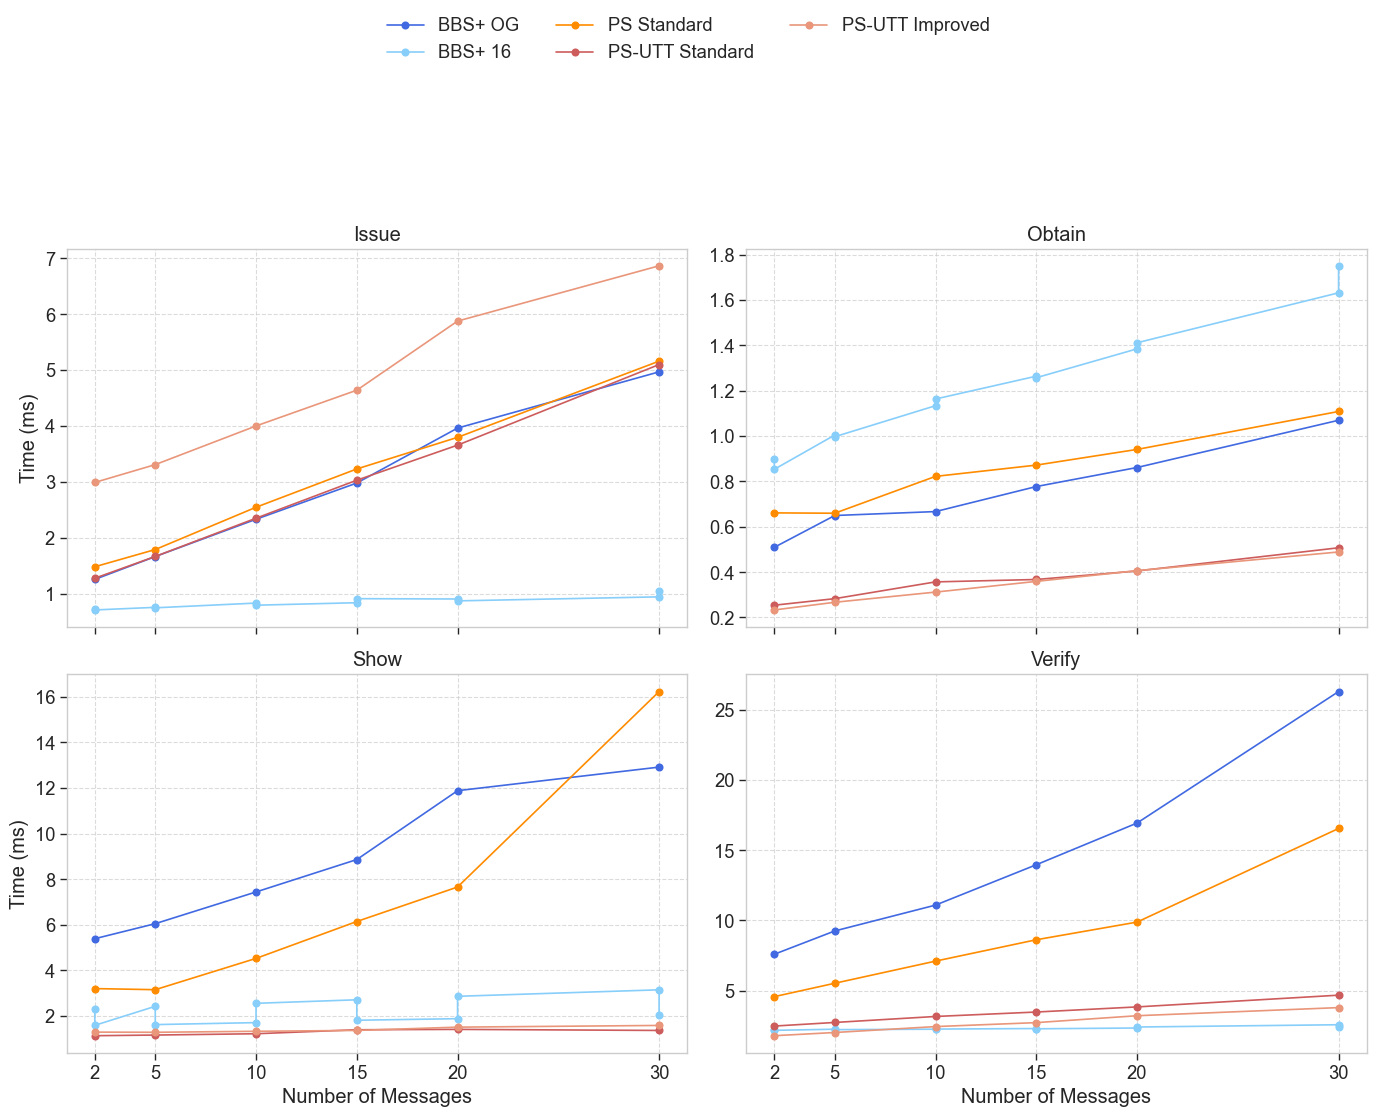
\includegraphics[width=1\linewidth]{comparison-line-graph.png}
    \caption{Performance Comparison of Anonymous Credential Schemes}
    
\end{figure}

\begin{figure}
    \centering
    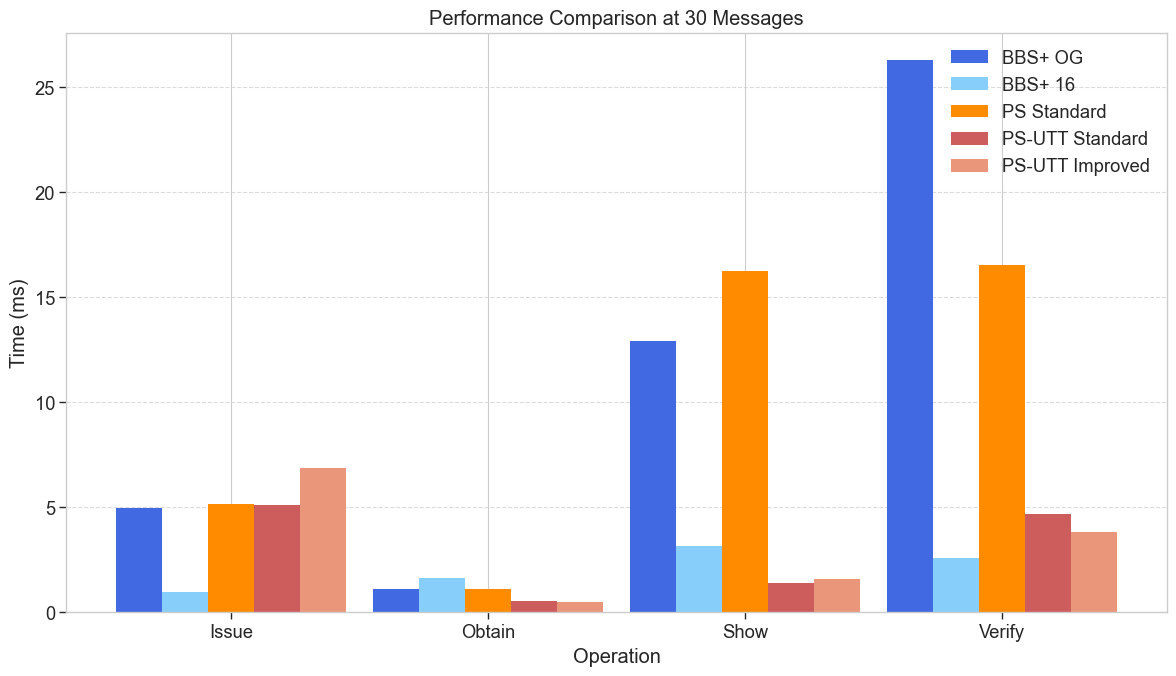
\includegraphics[width=0.7\linewidth]{performance-30.png}
    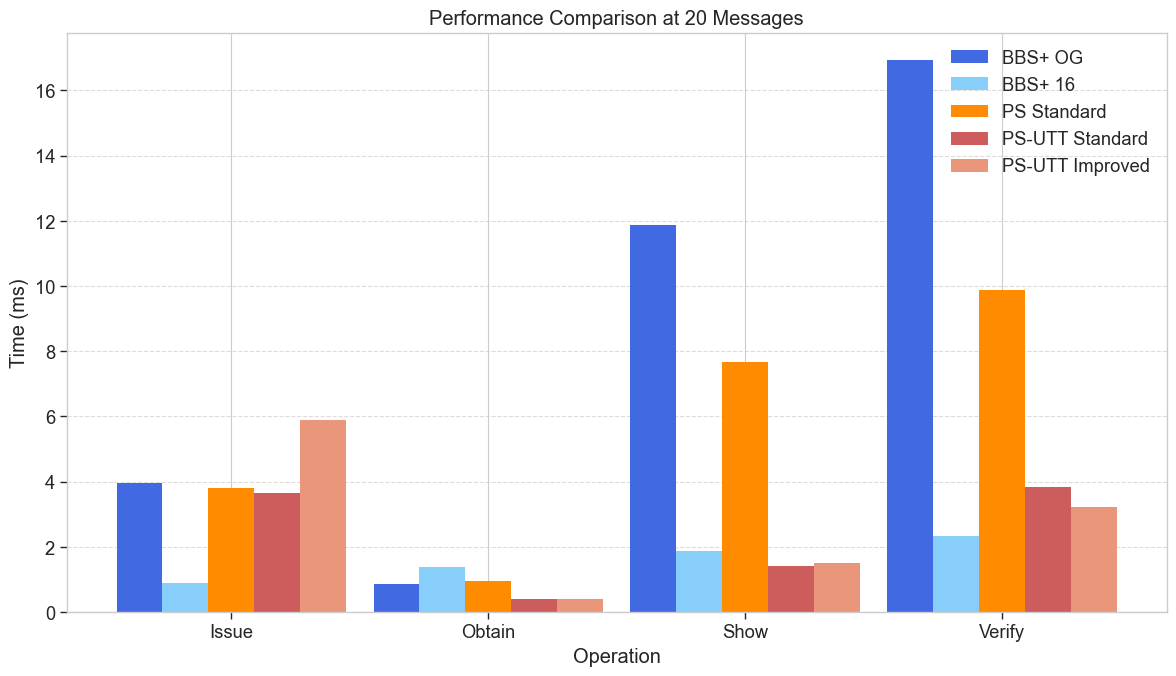
\includegraphics[width=0.7\linewidth]{performance-20.png}
    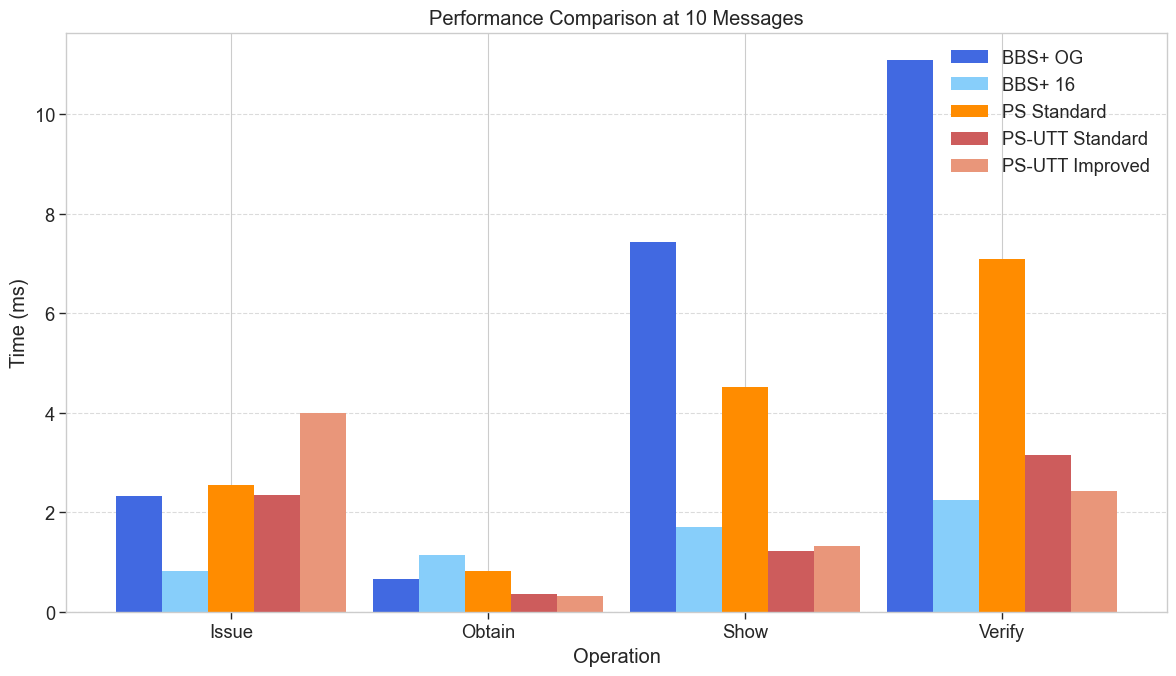
\includegraphics[width=0.7\linewidth]{performance-10.png}
     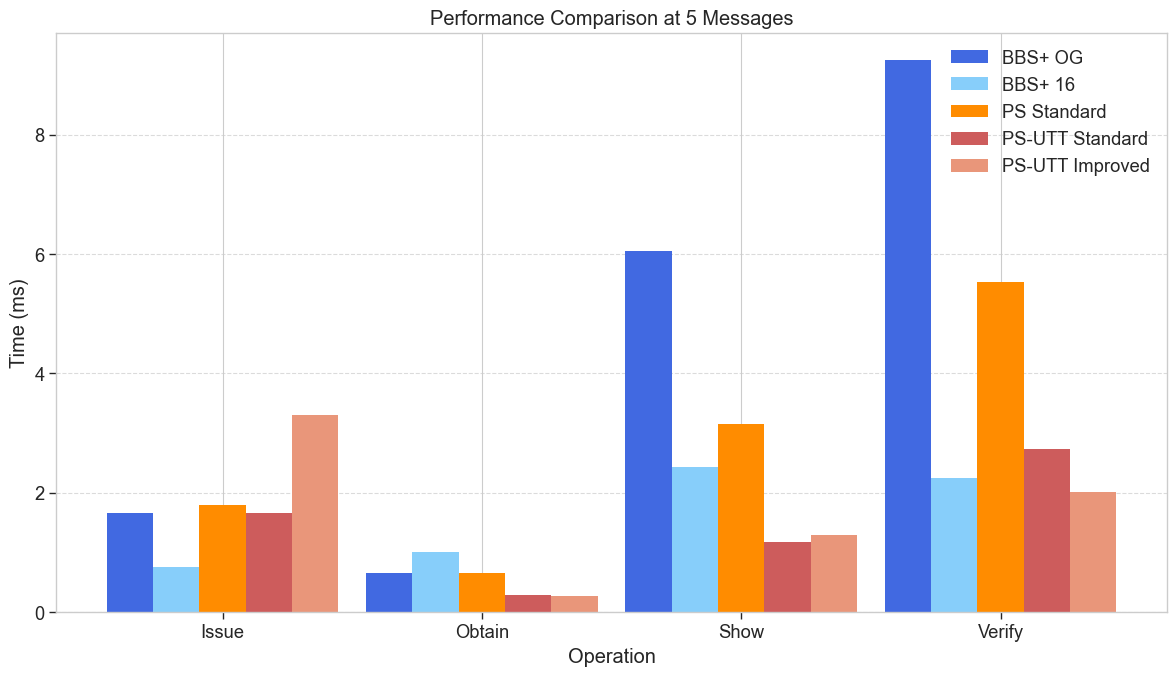
\includegraphics[width=0.7\linewidth]{performance-5.png}
    \caption{Performance Comparison of Anonymous Credential Schemes}
    
\end{figure}















\section{Summary}
- Both PS and BBS+ anonymous credentials use pedersen commitment schemes and sigma protocols for proving knowledge of committed attributes
- PS benefits structurally, rerandomization is much cleaner, and with our variant, show + verify time is more efficient
- Proving knowledge of the committed attributes in PS and BBS+ delivers the Schnorr responses that can be used to prove identity binding - we actually get this for free with no extra cost
- Sigma proofs are the most efficient and expressive proofs for proving knowledge of committed attributes. Although theoretically, they are linear in the size of the attributes, they are still extraordinarily efficient. Practical efficiencies in cryptography libraries such as MSM and batch techniques such as window tables and parallel computation reduce the practical complexity to, in many cases, log of the committed attributes. Polynomial commitments such as in the case of SPS-EQ improve the theoretical complexity but reduce the expressiveness of the proofs, further analysis needs to be done to benchmark the practical comparison. 
- A users transaction with a 30 message anonymous credential (large but not impossible) will cost approximately 5.37ms which is considered efficient in transactions. 
- For proving knowledge of multiple credentials together, the schnorr protocol used in both BBS+ and PS outputs a mechanism (equality of responses) to verify the identifier in each credential and therefore, this almost comes for free. 









\section{Improvement Notes}
Notes for performance summary improvements

Conduct multi-credential benchmarks: Instead of just saying "verification produces Schnorr responses, we can use those to verify multiple credentials at the same time," actually measure and report the end-to-end time for verifying multiple credentials with identity binding. This is your main contribution and should be the centerpiece of your evaluation.

Add a cost breakdown: Include a small table or graph showing the time spent in each cryptographic operation (exponentiations, pairings, etc.) to demonstrate where your optimizations matter most.


Connect to application requirements: Briefly discuss what performance is needed for practical deployment (e.g., "authentication should complete in <100ms for acceptable user experience") and how your results meet these targets.

Implementation Approach
When conducting the multi-credential benchmarks, you might structure the experiment like this:

Measure end-to-end time for Show+Verify with 1, 2, 3, 4, and 5 credentials from different issuers
For each case, verify a predicate that requires identity binding across all credentials
Compare against a naive approach where each credential is verified independently
If possible, compare against TACT or another system that supports multi-credential verification






9.1 Experimental Methodology
We implemented our MIMC-ABC system using the arkworks library [citation] in Rust. All experiments were conducted on a MacBook Air M2 (2022) with 16GB RAM. Each measurement represents the average of 10 independent trials with standard deviations below 5%.
Our evaluation focuses on three key dimensions:

Single-credential efficiency: We compare the computational cost of basic operations (Obtain, Issue, Show, Verify) across five schemes: BBS+ (2006) [citation], BBS+ (2016) [citation], PS (2016) [citation], PS-UTT G1 [citation], and our optimized PS-UTT G2.
Multi-credential scalability: We measure end-to-end verification time when presenting multiple credentials from different issuers, comparing our system against alternative approaches.
Identity binding overhead: We evaluate the additional cost of our identity binding mechanism, which ensures multiple credentials belong to the same identity.

For attribute vectors, we use parameter n to represent the number of attributes in each credential (ranging from 2 to 30). For multi-credential scenarios, parameter m represents the number of distinct credentials being verified simultaneously (ranging from 1 to 5).

% https://claude.ai/chat/b60de4f9-f2a8-4640-85b3-bc87474dbf65
% 9.3 Multi-Credential Performance
% While single-credential performance is important, our system's key innovation is efficient verification of multiple credentials from different issuers. Figure 3 shows the end-to-end verification time (including both Show and Verify operations) as we increase the number of credentials presented simultaneously.
% We compared three approaches:

% Naive aggregation: Simply performing independent verification for each credential (linear scaling)
% TACT [citation]: A recent system supporting multi-credential presentation
% Our MIMC-ABC: Our system with optimized G2 signatures and identity binding

% As shown in Figure 3, our approach demonstrates significantly better scaling as the number of credentials increases. For a predicate requiring 5 credentials from different issuers, our system completes verification in just 12.4ms—a 3.2× improvement over the naive approach (39.7ms) and 1.8× faster than TACT (22.8ms).
% The efficiency stems from two key factors:

% Our G2 signature optimization reduces pairing operations per credential
% The Schnorr responses generated during Show protocol allow efficient identity binding verification with minimal additional overhead

% Figure 4 isolates this second factor by measuring the specific cost of identity binding across credentials. The additional verification time remains nearly constant (~1.1ms) regardless of the number of credentials being bound, demonstrating the efficiency of our approach to identity binding.

% 9.4 Analysis and Discussion
% Our performance evaluation reveals several key insights about the efficiency of MIMC-ABC:
% Single-Credential Performance Tradeoffs
% Table 1 shows that our G2 optimization significantly improves verification time (up to 28% faster than PS-UTT G1) at the cost of slightly increased issuing time. This tradeoff is well-justified for anonymous credential systems where credentials are issued once but verified many times.
% The performance profile of BBS+ (2016) deserves special mention—it achieves the fastest issuing times and competitive verification for large attribute counts. However, as we'll discuss below, it doesn't scale as efficiently for multi-credential scenarios due to limitations in its proof structure.
% Multi-Credential Efficiency
% The most significant advantage of our system emerges in multi-credential scenarios. Figure 3 demonstrates that MIMC-ABC's verification time grows much more slowly with additional credentials compared to alternative approaches. This is particularly important for complex verification policies that require multiple credentials from different issuers.
% Specifically, our system exhibits near-linear scaling in the number of attributes (n) but sub-linear scaling in the number of credentials (m), thanks to the efficient reuse of Schnorr responses across credential proofs. This aligns perfectly with real-world usage patterns where users may have many credentials but typically present a small subset (3-5) for any given verification.
% Practical Implications
% For a typical scenario involving 5 credentials with 10 attributes each, our system completes the entire Show+Verify process in under 15ms, which is well below the 100ms threshold typically considered acceptable for interactive user experiences. This makes MIMC-ABC suitable for deployment in performance-sensitive contexts like mobile authentication.
% The performance profile also allows us to recommend specific parameter choices for implementations:

% For mobile clients: Limit attribute count to n≤15 to keep Show operations under 2ms
% For verification servers: Up to m=10 credentials can be verified simultaneously while maintaining sub-50ms response times





% \begin{table}[h]
% \centering
% \begin{tabular}{|l|r|}
% \hline
% \textbf{Operation} & \textbf{Time} \\
% \hline
% Full Pairing & 1.6218 ms \\
% Miller Loop & 0.6931 ms \\
% Final Exponentiation & 0.9287 ms \\
% G1 Mixed Addition (Affine + Jacobian) & 672 ns \\
% G1 Point Doubling (2P) & 414 ns \\
% G2 Mixed Addition (Affine + Jacobian) & 2143 ns \\
% G2 Point Doubling (2P) & 1302 ns \\
% \hline
% Estimated G1 Scalar Mult (255-bit) & 191.59 $\mu$s \\
% \emph{\small(255 doublings + ~128 additions)} & \\
% Estimated G2 Scalar Mult (255-bit) & 606.01 $\mu$s \\
% \emph{\small(255 doublings + ~128 additions)} & \\
% \hline
% \end{tabular}
% \caption{Performance metrics for arkworks BLS12-381 implementation. Scalar multiplication estimates assume naive double-and-add implementation without optimizations.}
% \label{tab:arkworks-performance}
% \end{table}
% \footnotetext{The G1 and G2 scalar multiplication estimates are derived using a naive double-and-add implementation analysis for 255-bit scalars. For a random scalar $k$, we assume approximately 255 doubling operations (one per bit) and 128 addition operations (corresponding to an expected Hamming weight of $\frac{255}{2}$ for a random scalar). The G1 estimate of 191.59$\mu$s is computed as $(255 \times 414\text{ns}) + (128 \times 672\text{ns})$ using the measured doubling and mixed addition timings. Similarly, the G2 estimate of 606.01$\mu$s is computed as $(255 \times 1302\text{ns}) + (128 \times 2143\text{ns})$. These estimates represent upper bounds as they do not account for common optimizations such as windowing methods, NAF (Non-Adjacent Form) representations, or parallel computation strategies.}








\section{Practical Proof Analysis}
\subsection{Sigma Protocols}
Many schemes refer to sigma protocol as having linear size proofs. 
While this is true in theory, using multi-scalar-multiplication, a popular algorithm in many cryptographic libraries, we show that sigma protocols are, in fact, sublinear rather than linear when message size doubles.

These findings support the hypothesis that practical efficiency is substantially better than theoretical complexity would suggest when using MSM in Schnorr protocols and thus the proof protocols in PS and BBS+ based anonymous credentials are sublinear in practice.

\begin{figure}
    \centering
    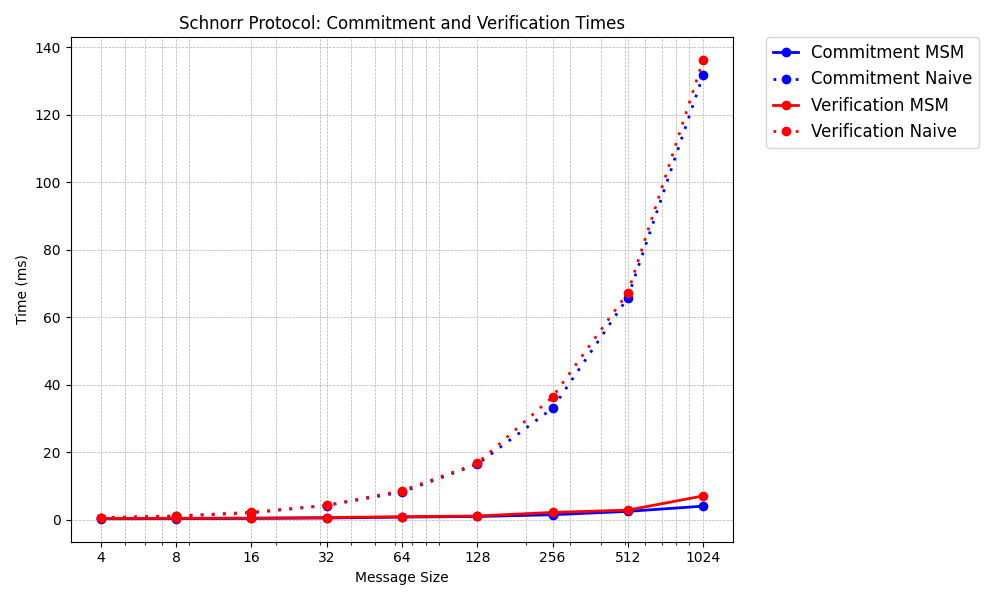
\includegraphics[width=0.75\linewidth]{schnorr_msm_no_msm.png}
    \caption{Schnorr Protocol - Practical Benchmarks with Multi-Scalar Multiplication}
    \label{fig:schnorr-benchmarks}
\end{figure}




\subsection{Pairing Protocols}

\begin{figure}
    \centering
    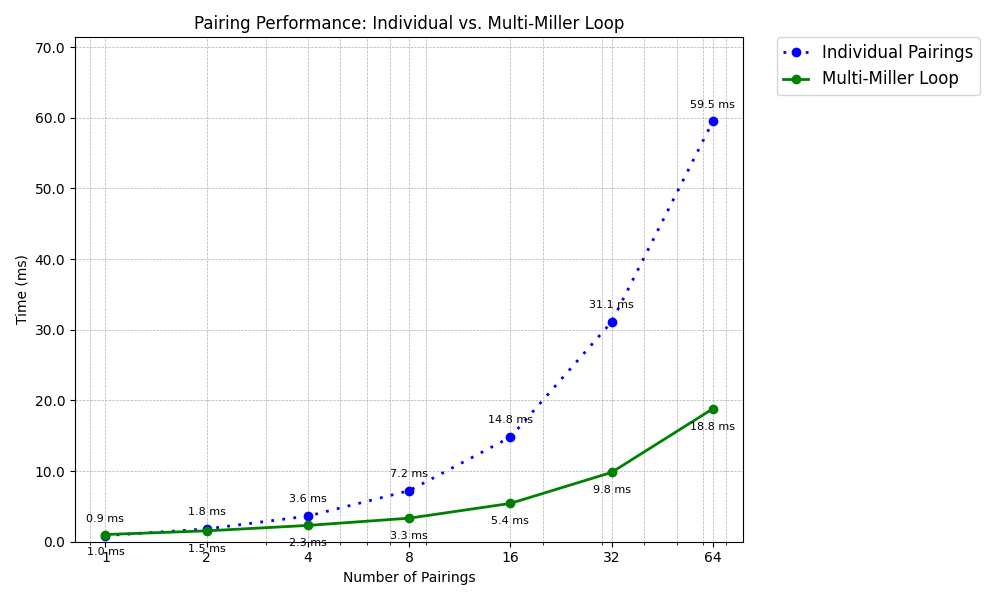
\includegraphics[width=0.75\linewidth]{pairing_comparison.png}
        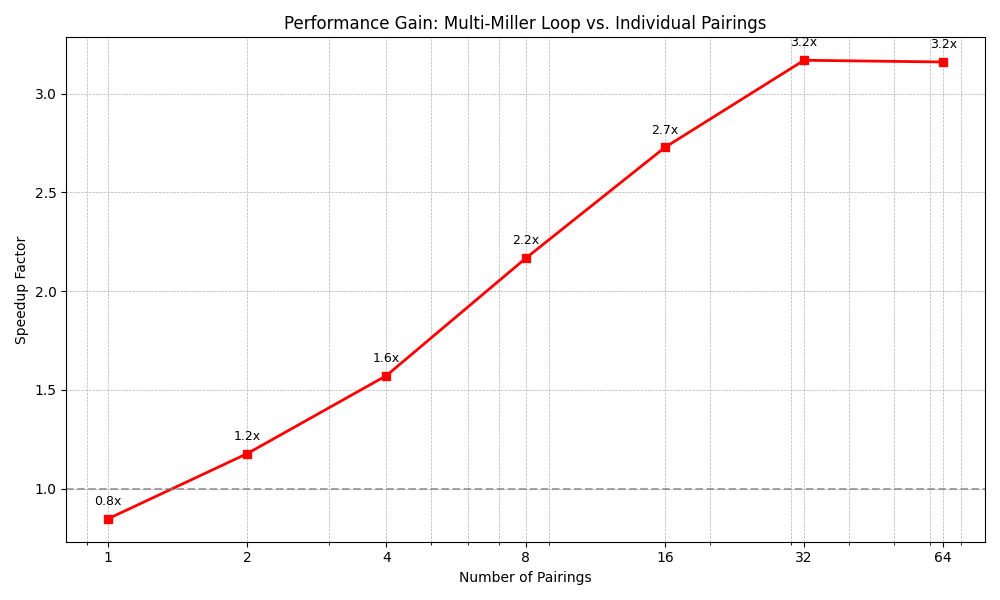
\includegraphics[width=0.75\linewidth]{pairing_comparison2.png}
    \caption{Elliptic Curve Pairings - Practical Benchmarks with Miller-Loop Intermediate Computation}
    \label{fig:enter-label}
\end{figure}

  % 
% Literature Review https://arxiv.org/pdf/2501.07209
% 
\newpage
\section{Appendix A}

\subsection{Pedersen Commitment Reduction}\label{appendix:commitmentreduction}
\begin{theorem}
    In the Algebraic Group Model, if the Symmetric Discrete Logarithm Problem (SDLP) is hard in the bilinear group $\BG$, then our Commitment scheme satisfies position binding. Specifically, for any algebraic PPT adversary $\mathcal{A}$ against position binding, there exists a PPT reduction $\mathcal{B}$ against SDLP such that:
    \[
        \mathsf{Adv}^{\mathsf{pos\text{-}bind}}_{\mathcal{A},\mathsf{RVC}}(\lambda) \leq \ell \cdot \mathsf{Adv}^{\mathsf{SDLP}}_{\mathcal{B},\mathbb{G}}(\lambda)
    \]
    where $\ell$ is the vector length.
\end{theorem}

\begin{proof}
We prove via reduction in the AGM. Given an algebraic PPT adversary $\mathcal{A}$ that breaks position binding with non-negligible probability $\epsilon$, we construct a PPT algorithm $\mathcal{B}$ that solves SDLP with probability $\epsilon/\ell$. For clarity, we illustrate with $\ell = 3$; the proof generalizes naturally.

Algorithm $\mathcal{B}$ works as follows:
\begin{enumerate}
    \item \textbf{Setup}: On input SDLP instance $(g^x, \tilde{g}^x) \in \mathbb{G}_1 \times \mathbb{G}_2$, $\mathcal{B}$ proceeds to:
    \begin{enumerate}
        \item Sample $i^* \sample [1,\ell]$ uniformly at random
        \item For position $i^*$: set $(g_{i^*}, \tilde{g}_{i^*}) \gets (g^x, \tilde{g}^x)$
        \item For positions $j \neq i^*$: sample $y_j \sample \mathbb{Z}_p$, set $(g_j, \tilde{g}_j) \gets (g^{y_j}, \tilde{g}^{y_j})$
        \item Give $\mathsf{ck} = ((g_1, g_2, g_3), (\tilde{g}_1, \tilde{g}_2, \tilde{g}_3))$ to $\mathcal{A}$
    \end{enumerate}
    
    \item \textbf{Position Binding Break}: Since $\mathcal{A}$ is algebraic, when it outputs $(\mathsf{cm}, i, \vec{m}_0, \vec{m}_1, r_0, r_1)$, it also provides the representation of $\mathsf{cm}$ in terms of the generators:
    \begin{itemize}
        \item $\mathsf{cm} \in \mathbb{G}_1$ with its algebraic representation
        \item $i \in [1,\ell]$ is the position where binding breaks
        \item $\vec{m}_0, \vec{m}_1 \in \mathbb{Z}_p^\ell$ differ only at position $i$
        \item $r_0, r_1 \in \mathbb{Z}_p$ are opening randomness values
    \end{itemize}
    
    \item \textbf{Extracting SDLP}: If $i \neq i^*$, abort. Otherwise:
    \begin{enumerate}
        \item By the algebraic property of $\mathcal{A}$, we have explicit representations of the commitment openings:
        \[
            g^{r_0}g_1^{m_{0,1}}g_2^{x \cdot m_{0,2}}g_3^{m_{0,3}} = g^{r_1}g_1^{m_{1,1}}g_2^{x \cdot m_{1,2}}g_3^{m_{1,3}}
        \]
        
        \item Since these representations are explicit in the AGM, we can directly compare exponents:
        \[
            r_0 + y_1m_{0,1} + xm_{0,2} + y_3m_{0,3} = r_1 + y_1m_{1,1} + xm_{1,2} + y_3m_{1,3}
        \]
        
        \item Since $\vec{m}_0$ and $\vec{m}_1$ differ only at position $i^*=2$, we have $m_{0,1}=m_{1,1}$ and $m_{0,3}=m_{1,3}$. Terms cancel:
        \[
            r_0 + xm_{0,2} = r_1 + xm_{1,2}
        \]
        
        \item Solve for $x$:
        \[
            x \equiv \frac{r_1-r_0}{m_{0,2}-m_{1,2}} \pmod{p}
        \]
        Note: Division is well-defined as $m_{0,2} \neq m_{1,2}$ by assumption.
    \end{enumerate}
\end{enumerate}

The reduction succeeds whenever $i = i^*$ and $\mathcal{A}$ succeeds, which occurs with probability $\epsilon/\ell$. This is non-negligible when $\epsilon$ is non-negligible, contradicting the SDLP assumption.
\end{proof}



We analyze the reduction's properties in detail:
\begin{itemize}
    \item \textbf{Perfect Simulation:} The commitment key distribution is identical to the real scheme:
        \begin{itemize}
            \item At position $i^*$: $(g_{i^*}, \tilde{g}_{i^*}) = (g^x, \tilde{g}^x)$ is uniformly distributed in $\G_1 \times \G_2$ by the SDLP instance properties
            \item At positions $j \neq i^*$: $(g_j, \tilde{g}_j) = (g^{y_j}, \tilde{g}^{y_j})$ is uniform due to $y_j \sample \Z_p$
            \item Therefore, from $\mathcal{A}$'s view, $\mathsf{ck}$ is distributed identically to the real scheme
        \end{itemize}
    
    \item \textbf{Extraction Success:} $\mathcal{B}$ successfully extracts the SDLP solution when:
        \begin{itemize}
            \item $\mathcal{A}$ outputs a valid position binding break (occurs with probability $\epsilon$)
            \item The guessed position matches: $i = i^*$ (occurs with probability $1/\ell$)
            \item The extraction equation is solvable: $m_{0,i^*} \neq m_{1,i^*}$ (guaranteed by definition of position binding break)
        \end{itemize}
    
    \item \textbf{Advantage Analysis:} Combining these probabilities:
        \begin{itemize}
            \item Events are independent as $i^*$ is chosen before $\mathcal{A}$'s execution
            \item $\mathsf{Pr}[\mathcal{B} \text{ succeeds}] = \epsilon \cdot \frac{1}{\ell}$
            \item Therefore: $\mathsf{Adv}^{\mathsf{SDLP}}_{\mathcal{B},\G}(\lambda) \geq \frac{1}{\ell} \cdot \mathsf{Adv}^{\mathsf{pos\text{-}bind}}_{\mathcal{A},\mathsf{RVC}}(\lambda)$
        \end{itemize}
\end{itemize}

Thus, if $\mathcal{A}$ breaks position binding with non-negligible probability $\epsilon$, then $\mathcal{B}$ solves SDLP with non-negligible probability $\epsilon/\ell$, contradicting the SDLP hardness assumption in $\G$.


\section{Appendix B}\label{app:zkp}
\subsection{Zero-Knowledge Proofs and Sigma-Protocols}

\subsubsection{Interactive Proof Systems}
An interactive proof system for a language $L$ involves a prover $\mathcal{P}$ and verifier $\mathcal{V}$, both probabilistic polynomial-time machines. For a statement $x$ and witness $w$ where $x \in L$, it satisfies:
\begin{itemize}
    \item \textbf{Completeness}: $\Pr[(\mathcal{P}(w), \mathcal{V})(x) = 1] \geq 1 - \negl(\lambda)$.
    \item \textbf{Soundness}: For any $\mathcal{P}^*$, if $x \notin L$, $\Pr[(\mathcal{P}^*, \mathcal{V})(x) = 1] \leq \negl(\lambda)$.
\end{itemize}
In our system, $\mathcal{P}$ is the user proving credential validity, and $\mathcal{V}$ is the verifier.

\subsubsection{Zero-Knowledge Property}
A proof is zero-knowledge if it reveals only that $x \in L$. Formally, for any $\mathcal{V}^*$, there exists a simulator $\mathcal{S}$ such that:
\[
\{\text{VIEW}_{\mathcal{V}^*}(\mathcal{P}(w), \mathcal{V}^*)(x)\} \approx_c \{\mathcal{S}(x)\}, \quad \forall x \in L.
\]
This property ensures anonymity in our $\textsf{Show}$ protocol (Section~\ref{sec:anonymity}).

\subsubsection{Proofs of Knowledge}
A proof is a proof of knowledge if an extractor $\mathcal{E}$, with rewind access to $\mathcal{P}^*$, can extract $w$ when $\mathcal{P}^*$ convinces $\mathcal{V}$ with non-negligible probability:
\[
\Pr[\mathcal{E}^{\mathcal{P}^*}(x) = w : (x, w) \in R] \geq \Pr[(\mathcal{P}^*, \mathcal{V})(x) = 1] - \negl(\lambda).
\]
This supports unforgeability (Section~\ref{sec:unforgeability}), ensuring only users knowing $\textsf{usk}$ can generate valid proofs.

\subsubsection{Sigma-Protocols}
A Sigma-protocol for a relation $R$ is a three-move protocol:
\begin{enumerate}
    \item $\mathcal{P}(x, w)$ sends commitment $a$.
    \item $\mathcal{V}$ sends challenge $e \leftarrow \{0,1\}^t$.
    \item $\mathcal{P}$ sends response $z$.
\end{enumerate}
$\mathcal{V}$ accepts if $\phi(x, a, e, z) = 1$. It satisfies completeness, special soundness, and SHVZK.

\subsubsection{Example: Schnorr’s Protocol}
For $\mathcal{R}_{\mathsf{DL}} = \{(h, w) \in \mathbb{G} \times \mathbb{Z}_q : h = g^w\}$, Schnorr’s protocol proves knowledge of $w$:
\begin{itemize}
    \item \textbf{Commitment}: $\mathcal{P}$ samples $r \leftarrow \mathbb{Z}_q$, sends $a = g^r$.
    \item \textbf{Challenge}: $\mathcal{V}$ sends $e \leftarrow \{0,1\}^t$.
    \item \textbf{Response}: $\mathcal{P}$ sends $z = r + e w \mod q$.
    \item \textbf{Verification}: $\mathcal{V}$ checks $g^z = a \cdot h^e$.
\end{itemize}
\textbf{Properties}:
\begin{itemize}
    \item \textbf{Completeness}: $g^z = g^{r + e w} = g^r \cdot (g^w)^e = a \cdot h^e$.
    \item \textbf{Special Soundness}: From $(a, e, z)$ and $(a, e', z')$, $w = (z - z') / (e - e') \mod q$.
    \item \textbf{SHVZK}: Simulator samples $z \leftarrow \mathbb{Z}_q$, sets $a = g^z h^{-e}$.
\end{itemize}


% Add examples of schnorr protocols

% Appendix A: Sigma Protocol Constructions

% A.1 Notation and Conventions
%     - Define witness notation, challenge spaces, etc.

% A.2 Proof of Commitment Opening
%     - Complete protocol description: P→V, V→P, P→V
%     - Simulator construction
%     - Extractor construction

% A.3 Signature Verification Proof
%     - Protocol for proving e(σ₂′, g̃) = e(σ₁′, vk·c̃m′)
%     - Optimizations for pairing-based operations

% A.4 Predicate Evaluation Proofs
%     - Techniques for AND/OR compositions
%     - Range proofs for inequality predicates
%     - Equality proofs across credentials
  \mychapter{}

\section{Multi Issuer Multi Credential Anonymous Credentials (MIMC-ABC)}\label{sec:mimc}


\subsection{Notation}
We base our Multi Issuer, Multi Credential Multi-show Attribute based Anonymous Credentials off the model in \cite{fuchsbauer_structure-preserving_2019} and extend it to support rerandomizable signatures over commitments and predicate-based zero-knowledge proof verification allowing users to prove statements about their committed and signed attributes without revealing any additional information.

\subsection{Predicate Satisfaction}
We define a predicate $\phi$ as a boolean function over an attribute vector $\vec{m}$, formally  $\phi: \mathcal{M} \rightarrow \{0,1\}$, where $\mathcal{M}$ is the space of the attribute vectors. 
For a credential with attributes $m = [\id, \ctx, \attrs]$, we say that "$m$ satisfies $\phi$", denoted as $\phi(m) = 1$, if the boolean function evaluates to true on the attributes.
For example, the predicate $\phi_{master} = \ctx = "master"$ is satisfied by $\vec{m} = [\id="123", \ctx="master", \attrs]$. Our system supports complex predicates such as $\phi = age > 18 \wedge country = US$ enabling expressive policies beyond simple equality checks. In our unforgeability definition, predicate satisfaction ensures an adversary cannot forge a proof for a predicate they do not legitimately satisfy beyond reusing existing credentials in a legitimate way.

\subsection{Syntax}
\begin{definition}[MIMC-ABC System] A Multi-Issuer Multi-Credential Attribute-based Anonymous Credential system consists of the following $\PPT$ algorithms:
    \begin{itemize}
    \item $\mathsf{Setup}(\secparam) \to (\ppar)$ Takes security parameter $\lambda$ in unary, outputs public parameters $\ppar$.
    
    \item $\mathsf{OrgKeygen}(\ppar, \ell) \to (\osk, \opk)$: Is a probabilistic algorithm that takes public parameters $\ppar$ and $\ell$ the upper bound of credential attributes. Outputs organisation's keypair $(\osk, \opk)$
       
    \item $(\mathsf{Obtain}(\vec{m}, \opk, \aux), \mathsf{Issue}(\osk, \cm, \aux)) \rightarrow (\cred, \bot)$ is an interactive protocol between a user and an issuing organization. The user inputs their message vector $\vec{m} = [\id, \ctx, \attrs]$ containing a unique identifier $\id$ and context $\ctx$. User generates $\usk \sample Z_p$, commits to their messages $\cm \gets \CMCom(\vec{m}; \usk)$. The issuer inputs their secret key $\osk$. The protocol outputs a credential $\cred$ containing $(\sigma, \cm)$ to the user and $\bot$ to the issuer.    
    
    \item $(\mathsf{Show}(\{\credi\}, \{\uski\}, \phi), \mathsf{Verify}(\{\credi'\}, \pi)) \rightarrow \{0,1\}$ is an interactive protocol between a user and verifier. The user runs $\mathsf{Show}$ with their credentials (signatures and paired commitments), and secret keys. The user rerandomizes their credentials and commitments and computes a proof $\pi$ that satisfies the predicate $\phi$.
    $\Verify$ is run by the verifier, which takes input from the randomized credentials $\cred_i'$, randomized commitments $\cmi'$, and predicate, proof pair $\phi, \pi$. The protocol outputs 1 if verification succeeds, 0 otherwise.
    \end{itemize}
\end{definition}

\newpage
\subsection{Security Model}
% Intuition of our security. 

% Here i Can talk about the different attack vectors and how the security of our system changes between single issuer, single credential, to multi credential to multiple issuer.

\subsubsection{Security Properties}

\begin{itemize}
    \item Correctness ensures an honest user with valid credentials can always generate a proof for any predicate their credentials satisfy which will verify with high probability

    \item Unforgeability prevents a malicious user, or colluding users, from creating valid proof for new forged credentials, misuse of legitimately issued ones, or unauthorized combination of credentials they don't own.

    \item Anonymity protects user privacy, ensuring proofs reveal only that the predicate is satisfied, even if adversaries control the issuers or define predicates. 
\end{itemize}

To model the adversary’s capabilities and the system’s state, we introduce the following lists and oracles:


\noindent\textbf{Lists}
\begin{itemize}
    \item $\HU$: The set of honest users whose secret keys remain unknown to the adversary $\adv$
    \item $\CU$: The set of corrupt users whose secret keys are known to the adversary $\adv$
    \item $\CRED_j$: A list tracking all credentials issued by issuer $j$, where each credential is associated with a user and their attributes
    \item $\OWNR$: A mapping from each credential to its owning user, i.e., $\OWNR[\cred] = i$ if credential $\cred$ belongs to user $i$
    \item $\SHOW$: A list tracking all credential show outputs (\{\})
\end{itemize} 

\noindent\textbf{Oracles}
\begin{itemize}
    \item $\OHU()$: Creates a new honest user $i$, adds them to $\HU$, and returns $i$
    \item $\OCU(i)$: Corrupts user $i$ by moving them from $\HU$ to $\CU$, revealing their secret keys (e.g., commitment openings) and all credentials ${\cred}$ owned by $i$
    \item $\OOBTAIN(i, j, \vec{m})$: Issues a credential $\cred$ from issuer $j$ to user $i$ for the attribute vector $\vec{m}$, provided $i \in \HU$. The credential is added to $\CRED_j$, and $\OWNR[\cred]$ is set to $i$
    \item $\OSHOW(i, \phi)$: Generates a proof $\pi$ that the credentials of user $i$ satisfy the predicate $\phi$, provided $i \in \HU$ and the credentials meet the condition $\phi$. $\SHOW \cup \SHOW \{i, \pi\}$
\end{itemize} 



\begin{definition}[Correctness]
    \[
        \Pr \left[ 
            \Verify(\{\cred_k'\}, \{\cm_k'\}, \phi, \pi) = 1 \mid \text{all steps honest} \wedge \phi(\{m_k\}) = 1
        \right] = 1 - \negl[\lambda]
    \]
\end{definition}

\paragraph{Intuition:} A MIMC-ABC system is correct if, when all parties follow the protocol honestly, a user can successfully prove a true statement about their credentials to a verifier. Specifically, for all honestly generated public parameters, keys, credentials, and predicates satisfied by the user’s attributes, the verification process accepts the proof with overwhelming probability. 

    \begin{itemize}
        \item \textbf{Setup:} Challenger $\AdvC$ runs $\Setup(\secparam) \to \ppar$
        \item \textbf{Issuer Keys:} For each issuer $j$ in a set of issuers $\{j\}$, run $\OrgKeyGen(\ppar, \ell) \to (\osk_j, \opk_j)$.
        \item \textbf{Credential Issuance: } For a set of message vectors $\{m_k\}$, each $m_k = [\id, \ctx, \attrs, \usk_k]$ with the same $\id$. User runs $\UserKeyGen(\ppar) \to \usk_k$ and $\Obtain(\ppar, \opk_j, m_k, \aux),\Issue(\osk_j, \cm_k, \aux) \to \{\cred_k\}$. 
        \item \textbf{Proof Generation:} User runs $\Show(\{\cred_k'\}, \{\cm_k'\}, \phi, \pi)$ where $\{\cred_k'\}$ and $\{\cm_k'\}$ are rerandomized credentials and commitments.
        \item \textbf{Winning Condition:} Correctness holds if $\Verify(\{\cred_k'\}, \{\cm_k'\}, \phi, \pi) = 1 $ with $\Pr = 1-\negl[\lambda]$
    \end{itemize}
More formally,















\begin{definition}[Unforgeability]
A MIMC-ABC system is unforgeable if for all PPT adversaries $\mathcal{A}$, there exists a negligible function $\negl$ such that:
\[
\mathsf{Adv}\left[\mathrm{Game}^{\mathsf{\UNF}}_{\MIMCABC, \adv}(\lambda) = 1\right] \leq \negl[\secparam]
\]
\end{definition}

\paragraph{Intuition:} A MIMC-ABC system is unforgeable if no probabilistic polynomial-time (PPT) adversary can produce a valid proof for a predicate that they cannot legitimately satisfy, based on the credentials they have obtained or corrupted. This prevents \emph{forging credentials} or \emph{proving false statements} about them including faking identity binding and credential relationships when stated by $\phi$.

\paragraph{The intuition for the forgery success condition}: The adversary's forgery is successful if their proof verifies correctly \emph{and} the credentials used in the forgery cannot be traced back to a single corrupted user. The trivial forgery is one where the adversary corrupts a user and verifies a statement with their legitimately issued credentials. The adversary can win by combining credentials from multiple corrupt users to create valid proofs, combining credentials from corrupt users with newly forged credentials, and lastly creating entirely forged credentials. This is where our security properties, Identity Binding, and Credential Relationship Binding stem from.

\begin{remark}
    For \emph{identity binding}, if $\phi^*$ requires all $\id$ to match, $\AdvA$ can't mix credentials from different $\id$'s. For \emph{credential relationship binding}, if $\phi^*$ requires a specific relationship, for example $\cred_1$ contains $\CMCom([\id, \ctx="passport", \attrs]) \wedge \cred_2$ contains $\CMCom([\id, \ctx="driversLicense", \attrs])$ then $\AdvA$ can't win with different $\ctx$ or use something in $\attrs$ to satisfy $\phi^*$
    
\end{remark}



\begin{definition}[MIMC-ABC Anonymity]
A MIMC-ABC system provides anonymity if, for all PPT adversaries $\adv$, the advantage in the following experiment is negligible:
\[
\mathsf{Adv}^{\mathsf{anon}}_{\adv}(\secparam) = \left| \Pr[\mathrm{Game}^{\mathsf{anon-1}}_{\MIMCABC, \adv}(\secparam) = 1] - \Pr[\mathrm{Game}^{\mathsf{anon-0}}_{\MIMCABC, \adv}(\secparam) = 1] \right| \leq \negl(\lambda)
\]
\end{definition}

\begin{figure}
    \centering
    \begin{pcvstack}[boxed, center, space=1em]
        \begin{pchstack}
                 \begin{pcvstack}
                 \procedure[linenumbering]{$\mathrm{Game}^{\mathsf{\UNF}}_{\MIMCABC, \adv}(\secparam)$}{%
                    \pccomment{Challenger Setup} \\
                    \text{Initialize } \HU \gets \emptyset, \CU \gets \emptyset, \\
                    \CRED_j \gets \emptyset \text{ for each $j$}, \OWNR \gets \{\} \\
                    \ppar \gets \Setup(\secparam), (\osk_j, \opk_j) \gets \OrgKeyGen(\ppar) \\
                    \pccomment{$\AdvA$ queries oracles} \\
                    \AdvA^{\OHU, \OCU, \OOBTAIN}(\opk_j) \\
                    \pccomment{Forgery} \\
                    \AdvA \text{ outputs } (\{\cred_k'^*\} = (\{\sigma_k'^*, \cm_k'^*\}) ) \\
                    \pccomment{Winning Condition} \\
                    \Verify(\{\cred_k'^*\}, \phi^*, \pi^*, \{\opk_j\}) = 1 \; \wedge \\
                    \t \forall k, \OWNR[\{\cred_k'^*\}] \neq i \in \CU \quad \pclinecomment{Version 1}\\
                    \t \nexists i \in \CU : \phi^*(\vec{m}_{i,k}) = 1 \quad \pclinecomment{Version 2}\\
                    \pccomment{i.e. the set of all $\{\cred_k'^*\}$} \\
                    \pccomment{cannot belong to the same corrupt user}
                }
            \end{pcvstack}
             \begin{pcvstack}
             \procedure[linenumbering]{$\mathrm{Game}^{\mathsf{\ANON}}_{\MIMCABC, \adv}(\lambda)$}{%
                    \ppar \gets \Setup(\secparam), \HU, \gets \emptyset, \CU \gets \emptyset \quad \pclinecomment{Challenger $\AdvC$ Setup} \\
                    \{\osk_j, \opk_j\} \gets \AdvA(\OrgKeyGen(\ppar)) \text{ for each issuer $j$}. \\
                    \text{For $i$ in } \bit: \qquad \pclinecomment{$\AdvC$ initializes two honest users }\\
                    \t \usk_i \gets \UserKeyGen(\ppar), \HU \gets \HU \cup \{i\}, \\
                    \t \quad i \text{ has } \vec{m} \text{ such that } \phi(\vec{m}) = 1 \\
                    \t \cm_i \gets \CMCom(\vec{m}_i; \usk_i),  \cred_i \gets \Issue(\osk, \cm_i) \\
                    \AdvA^{\OHU, \OCU, \OOBTAIN, \OSHOW}(\{\osk_j, \opk_j\} ) \qquad \pclinecomment{Learning Phase} \\
                    (i_0, i_1, \phi) \gets \AdvA() \qquad \pclinecomment{Challenge Phase}\\
                    \text{Assert } i_0, i_1 \in \HU \setminus \CU, \quad \wedge \quad \phi(\vec{m}_{i_0}) = 1, \phi(\vec{m}_{i_1}) = 1 \\
                    b \sample \bit \quad \pclinecomment{$\AdvC$ samples random bit}\\
                    (\cred', \cm', \pi) \gets \Show(\creds_{i_b}, \cm_{i_b}, \usk_{i_b}, \phi)\\
                    b' \gets \AdvA(\cred', \cm', \pi) \qquad \pclinecomment{$\AdvA$ guesses who's $\cred$ it is } \\
                    \text{Return } (b' = b), \pclinecomment{Wins with the correct guess}}
            \end{pcvstack}
        \end{pchstack}
        \end{pcvstack}
    \caption{Caption}
    % 
\end{figure}

\begin{figure}
    \centering
\begin{pchstack}[boxed]
        \begin{pcvstack}
            \procedure[]{$\OHU()$}{%
                \pcif i \notin \HU \cup \CU \\
                \t \HU \gets \HU \cup \{i\} \\
                \pcreturn  i \\
            }
            \procedure[]{$\OCU(i)$}{%
                \pcif i \in \HU:\\
                \t \HU \gets \HU \setminus \{i\} \\
                \t \CU \gets \CU \cup \{i\} \\
                \t \creds_i \gets \{\cred | \OWNR[\cred] = i\} \\
                \t \pcreturn \{(\cred, \usk) | (\cred, \cm, \vec{m}, \usk, i, j) \in \CRED\}\\
                \pcreturn \bot \\
            }
        \end{pcvstack}
        \begin{pcvstack}
            \procedure[]{$\OOBTAIN(i, j, \vec{m})$}{%
                \pcif i \in \HU: \\
                \t \usk \sample \Z_p \\
                \t \cm \gets \CMCom([\vec{m}]; \usk) \\
                \t \cred \gets \Issue(\osk_j, \cm) \\
                \t \CRED \gets (\cred, \cm, \vec{m}, \usk, i, j), \\
                \t \OWNR[\cred] = i \\
                \pcreturn \cred \\
            }
            \procedure[]{$\OSHOW(i, \creds_i, \phi)$}{%
                \pcif i \in \HU \; \wedge \; \phi(\creds_i) = 1: \\
                \t \text{Parse } \creds = \{\sigma, \cm, \vec{m}, \usk \} \\
                \t \pi \gets \Show(\creds_i, \phi) \\
                \t \pcreturn \pi \\
                \pcreturn \bot \\
            }
        \end{pcvstack}
    \end{pchstack}
    \caption{Caption}
    \label{}
\end{figure}


\paragraph{Anonymity: }A MIMC-ABC system provides anonymity if no PPT adversary can determine which user’s credentials were used in a proof, even if the adversary controls the issuers and chooses the messages and predicates. This ensures that presentations reveal only what the predicate explicitly requires, protecting user privacy.

\paragraph{Intuition}: the challenger sets up the game by picking a random bit $b \sample \bit$, which decides whether it uses "Alice or Bob's" credential in the game. Based on the bit, the challenger generates a credential "show" proof and presents it to the adversary. The adversary's guess should be no better than guessing.


























\newpage
\section{Construction}

\subsection{Intuition of Construction}

\subsubsection{Outline}
Our credential system operates over attribute space $\Z_p$. The user is indexed by $i$, the issuer by $j$, and the $k^{th}$ credential issued to user $i$ from issuer $j$. The credential $\cred$ is a rerandomizable Pointcheval-Sanders signature over commitments $\sigma \gets \mathsf{RS.Sign}(\cm, \mathsf{osk})$ where $\cm \gets \CMCom(\vec{m}; \usk)$. During verification, the user rerandomizes both signature and commitment for anonymity, then uses $\Sigma$-protocols to prove their correctness for any predicate $\phi$. This approach leverages the algebraic structure of PS Signatures and Pedersen Commitments, that is, messages are exponents of a commitment which yields well-known, highly expressive and efficient zero-knowledge proofs of group element exponents, supporting a wide range of statements from selective disclosure to complex arithmetic relations. However, proofs are linear in the number of exponents. In contrast, SPS-EQ \cite{fuchsbauer_structure-preserving_2019, hanaoka_improved_2022} use constant-size set commitments and although proofs have limited expressiveness, they are constant size and very efficient. On the other hand, \cite{rabaninejad_attribute-based_2024} use Groth-Sahai proofs. During $\Obtain, \Issue$, the user sends the commitment $\cm$ along with a proof of opening $\pircom(\cm)$ allowing the extraction of $\usk$ for corrupt users in the unforgeability proof.

\subsubsection{Example}
Consider a user holding credentials from three issuers, denoted $j = 1, 2, 3$, each providing one credential $k = 1$. The user rerandomizes each credential’s commitment and signature as follows: $\cm_{j,1}' \gets \CMRand(\cm_{j,1}, \Delta_{r_{j,1}})$ and $\sigma_{j,1}' \gets \RSRand(\sigma_{j,1}, \Delta_{r_{j,1}}, \Delta_{u_{j,1}})$. These rerandomized pairs $(\cm_{j,1}', \sigma_{j,1}')$ are indistinguishable from their original issuance. In the $\Show$ protocol, the verifier confirms their validity: $\RSVer(\sigma_{j,1}', \cm_{j,1}', \vk_j) = 1$ for all $j \in \{1, 2, 3\}$.

\begin{figure}
        \begin{pchstack}[boxed, center, space=4em]
            \begin{pcvstack}
                \procedure[space=auto]{Passport}{%
                \id: 12345, \\
                \ctx: "passport", \\
                \attrs: \mathsf{values}
                }
            \end{pcvstack}
            \pcvspace
            \begin{pcvstack}
                \procedure[space=auto]{Driver License}{%
                 \id: 12345, \\
                \ctx: "dmv", \\
                 \attrs: \mathsf{values}
                }
            \end{pcvstack}
            \pcvspace
            \begin{pcvstack}
                \procedure[space=auto]{University Degree}{%
                 \id: 12345, \\
                \ctx: "usyd{-}bcompsc", \\
                \attrs: \mathsf{values}
                }
            \end{pcvstack}
        \end{pchstack}
    \caption{Three Example Credentials, $\attrs$ holds arbitrary number of attributes such as expiry}
    \label{fig:three-creds}
\end{figure}

Next, the user proves a relation $\mathcal{R}_\phi$ that ensures the credentials satisfy a predicate $\phi$. 
\[
\mathcal{R}_\phi = \left\{ 
\begin{array}{l} 
\forall j, k: \RSVer(\sigma_{j,k}', \cm_{j,k}', \vk_j) = 1 \\ 
\forall j, k: \cm_{j,k}' = \CMRand(\CMCom([\id, \ctx_{j,k}, \attrs_{j,k}]; \usk_{j,k}), \Delta_{r_{j,k}}) \\ 
\phi(\{\ctx_{j,k}, \attrs_{j,k}\}) = 1 
\end{array} 
\right\}
\]

For instance, if $\phi$ requires a valid passport, driver’s license, and university degree, $\mathcal{R}_\phi$ might enforce $\ctx_{1,1} = \text{''passport''}$, $\attrs_{1,1}.\exp > \text{today}$, $\ctx_{2,1} = \text{''dmv''}$, and $\ctx_{3,1} \in \mathcal{D}$ (a set of accredited universities), with all commitments sharing the same $\id$.


\subsection{Sigma-protocol and core relations}

Our MIMC-ABC system relies on five core relations proven via $\Sigma$-protocols:
\begin{enumerate}
    \item \textbf{Commitment Opening:} For commitment $\cm$ to message vector $\vec{m} = [\id, \ctx, \attrs]$. $\pircom(\cm)$ is a proof for relation:
    \[
     \rcom = \zkpok \left\{(\cm, (\id, \ctx, \attrs, \usk))| \cm = g_1^{\id}g_2^{\ctx},\attrs, g^{\usk} \right\}
    \]
    
    \item \textbf{Signature Validity:} after rerandomization, our signatures in the form $\sigma' = (\sigma_1', \sigma_2')$ combine pairing verification with sigma protocol to prove knowledge of the committed messages and randomization factor. $\pirsigma$ is a proof for relation:
         \[
    \rsigma = \zkpok \left\{ 
    \begin{array}{l} 
    (\sigma', \cm', (\ctx, \attrs, \usk + \Delta_{\usk})) \\
    \end{array} 
    \middle|
    \begin{array}{l}
    e(\sigma_1, \vk \cdot \widetilde{\cm}) = e(\sigma_2, \tilde{g}) \quad \wedge \\
    e(\cm, \tilde{g}) = e(g, \widetilde{\cm}) \quad \wedge\\
    \cm = g_1^{\id}g_2^{\ctx},\attrs, g^{\usk + \Delta_\usk} \\
    \end{array} 
    \right\}
    \]


    \item \textbf{Identity Binding:} For two credentials with commitments $\cm_1$ and $\cm_2$:

    \[
    \rid = \zkpok \left\{ 
    \begin{array}{l} 
    (\cm_1, \cm_2, (\id, \usk_1, \usk_2, \ctx_1, \ctx_2, \attrs_1, \attrs_2)) \\
    \end{array} 
    \middle|
    \begin{array}{l}
    \cm_1 = g^{\usk_1} \cdot g_1^{\id} \cdot g_2^{\ctx_1} \cdot \prod g_i^{\attrs_{1,i}} \wedge \\
     \cm_2 = g^{\usk_2} \cdot g_1^{\id} \cdot g_2^{\ctx_2} \cdot \prod g_i^{\attrs_{2,i}} \\
    \end{array} 
    \right\}
    \]
    
    This proves both credentials share the same $\id$ without revealing the $\id$ value. This generalizes to $n$ credentials by proving equality across all $n$ commitments.
    
    The position-binding property of our commitment scheme (Section \ref{sec:commitment}) ensures this equality relation can't be forged - an adversary can't make two commitments appear to share the same $\id$ when they actually don't.

    \item \textbf{Malicious Issuer Protection:} For verification key $\vk$ and commitment key $\ck$, $\pirverkey$ is a proof for relation:
    \[
    \mathcal{R}_{\mathsf{verkey}} = \{(\vk, \ck, (\sk, x, \{y_i\}_{i=1}^{\ell})) \mid \sk = g^x \wedge \vk = \tilde{g}^x \wedge 
    \forall i \in [1,\ell]: g_i = g^{y_i} \wedge \tilde{g}_i = \tilde{g}^{y_i} \}
    \]
    
    This relation proves the issuer knows the discrete logarithms of their public keys, ensuring they can't create malformed keys that might enable deanonymization or signature forgery. The issuer must provide this proof during credential issuance, preventing attacks that exploit maliciously crafted keys with hidden structures.     

     \item \textbf{Predicate Satisfaction:} For credentials with attributes that satisfy a policy $\phi$:
    \[
    \mathcal{R}_{\phi} = \{(\{\cm_j\}, (\{\attrs_j\})) \mid \forall j: \cm_j \text{ correctly commits to } \attrs_j \wedge
    \phi(\{\attrs_j\}) = 1 \}
    \]
    
    A predicate $\phi$ is simply a policy statement about attributes that is satisfiable by the supported algebraic constraints in Sigma protocols, noting that sigma protocols are extremely expressive and can  . For example:

    These can be composed to support complex policies while maintaining zero-knowledge properties, revealing nothing beyond the fact that the policy is satisfied.
    \begin{itemize}
    \item ``age > 18'' (for a single credential)
    \item ``has valid driver's license AND passport'' (requiring multiple credentials)
    \item ``degree = 'Computer Science' AND university in accredited\_list''
    \end{itemize}
    
    The $\Sigma$-protocol allows proving these statements are true without revealing the actual attribute values, only that they satisfy the predicate $\phi$.

    
    The $\Sigma$-protocol framework allows for highly expressive predicates $\phi$ including:
    \begin{itemize}
    \item \textbf{Boolean operations:} AND, OR, and NOT compositions of simpler predicates
    \item \textbf{Arithmetic relations:} Equality, inequality ($<$, $>$, $\leq$, $\geq$), and linear combinations 
    \item \textbf{Range proofs:} Demonstrating a value lies within a specific range (e.g., ``18 $\leq$ age $<$ 65'')
    \item \textbf{Set membership:} Proving an attribute belongs to an approved set without revealing which one
    \item \textbf{Cross-credential relations:} Equality of attributes across different credentials (e.g., name matches across passport and driver's license)
    \end{itemize}

    
\end{enumerate}


\subsection{Security Mechanisms}

\subsubsection{Identity Binding}
Identity binding leverages the position-binding property of our commitment scheme. When proving multiple credentials belong to the same identity:
\begin{itemize}
    \item Prover demonstrates $\id_1 = \id_2 = \ldots = \id_n$ via $\Sigma$-protocol equality proof
    \item Position-binding prevents credential mixing attacks
    \item Breaking identity binding reduces to breaking position-binding (SDLP assumption)
\end{itemize}

\subsubsection{Credential Relationships}
Our system, and underlying $\Sigma$-protocols support credential relationship proofs:
\begin{itemize}
    \item Credential derivation $\cred_a \to \cred_b$
    \item Cross-credential attribute consistency
    \item Hierarchical credential verification
    \item Sybil-resistant nullifiers
\end{itemize}
These are implemented through $\Sigma$-protocol compositions on cross-credential attributes.

\subsubsection{Freshness}
We prevent replay attacks via the challenge phase of our $\Sigma$-protocols~\cite{desmedt_proofs_1994, damgard_sigma_2010}. Verifiers send random challenges that provers must incorporate into their responses. This approach requires no persistent state for verifiers and prevents cross-verifier-proof reuse. Non-interactive versions via Fiat-Shamir~\cite{odlyzko_how_1986} would require tracking used proofs.

\subsubsection{Malicious Organization Keys}
To prevent attacks from malicious issuers, we extend our signature scheme with:
\begin{itemize}
    \item $\mathsf{RS.VerKey}(\sk, \vk, \ck) \to \bit$: Verifies issuer keys via relation:
\end{itemize}
\[
\mathcal{R}_{\mathsf{verkey}} = \{(\vk, \ck),(\sk, x, \{y_i\}_{i=1}^\ell) \mid \sk = g^x \wedge \vk = \tilde{g}^x \wedge \bigwedge_{i=1}^\ell (g_i = g^{y_i} \wedge \tilde{g}_i = \tilde{g}^{y_i})\}
\]

This prevents deanonymization via specially crafted keys, and signature forgery via hidden key relationships. In security proofs, extractability enables reductions to standard cryptographic assumptions.


\newpage
\subsection{\MIMCABC Construction}
The Credential is a signature $\sigma$ over commitment $\cm = \mathsf{CM.Com}([\id, \ctx, \attrs]; \usk)$ where $\attrs$ represents ancillary committed messages which we do not focus on in our protocol. $j$ indexes the issuers, and $k$ indexes the credentials from a specific issuer. 

\begin{figure}
    \begin{center}
    \begin{tabular}{l@{\hspace{5em}}c@{\hspace{5em}}l}
    \multicolumn{3}{l}{$\underline{\mathsf{OrgKeyGen}(1^{\lambda}, 1^\ell, j)}$ for issuer $j$ and $\vec{m}$ length = $\ell$} \\[1em]
    \multicolumn{3}{l}{$\BG = (\G_1, \G_2, \G_T, e, g, \tilg,p) \sample \BGGen(\secparam), \; \mathsf{ck_j} \sample \mathsf{CM.Setup}(\BG, \secparam, \ell)$}\\[1em]
    \multicolumn{3}{l}{$(\sk_j, \vk_j) \sample \mathsf{RS.KeyGen}(\mathsf{ck}_j), \; \text{ Return } (\osk_j, \opk_j) = ((\sk_j),(\vk_j, \ck_j))$}\\[1em]
    \multicolumn{3}{l}{$\underline{\mathsf{(Obtain, Issue)}}$:}\\[1em]
    \multicolumn{3}{l}{$\pircom(\cm) = \zkpok\{(\id, \ctx, \attrs, \usk)| \cm = g_1^{\id}g_2^{\ctx},\ldots, g^{\usk} \}$}\\[1em]
    \multicolumn{3}{l}{$\pirverkey(\sk, \vk, \ck) = \zkpok\{(\sk, x, \{y_i\}_{i=1}^\ell) | \sk = g^x \wedge \vk = \tilde{g}^x \bigwedge_{i=1}^\ell (g_i = g^{y_i} \wedge \tilde{g}_i = \tilde{g}^{y_i})\}$}\\[1em]
    $\underline{\mathsf{Obtain}(\vec{m}, \opk)}$ && $\underline{\Issue(\pircom, \cm, \osk)}$ \\[1em]
    If  $\pirverkey(\sk, \vk, \ck)$ fails, return $\bot$ & $\xleftarrow{\pirverkey(\sk, \vk, \ck)}$ & \\[1em]
    $\usk \sample \Z_p, \cm = \CMCom([\id,\ctx, \attrs];\usk)$ & $\xrightarrow{\;\; \pircom(\cm) \;\;}$ & \;\; If $ \pircom(\cm)$ fails, return $\bot$ \\[1em]
    If $\RSVer(\sigma, \cm, \opk) = 0$, return $\bot$  & $\xleftarrow{\qquad \sigma \qquad}$ & $u \sample \Z_p$, $\sigma \sample \RSSign(\cm, \osk, u)$ \\[1em]
    \multicolumn{3}{l}{\; Else, return $\cred_{j,i} \gets (\sigma, \cm, \usk, \opk_j)$} \\[1em]
    \multicolumn{3}{l}{$\underline{(\mathsf{Show}, \mathsf{Verify}):}$ for a set $\{\cred_{j,k}\}$ and predicate $\phi$:}\\[1em]
    \multicolumn{3}{l}{$\Pi_\phi = \zkpok\{(\{\id, \ctx_{k}, \attrs_{j,k}, \usk_{j,k}'\}_{j,k}) \; | \; \forall j,k: \cm_{j,k}' = \CMCom([\id, \ctx_{k}, \attrs_{j,k}]; \usk_{j,k}') \wedge$} \\[0.5em]
    \multicolumn{3}{l}{\quad $\RSVer(\sigma_{j,k}', \cm_{j,k}', \opk_j) = 1 \; \wedge \; \phi(\{[\id, \ctx_{k}, \attrs_{j,k}]\}_{j,k}) = 1 \}$}\\[1em]
    $\underline{\mathsf{Show}(\{\cred_{j,k}\}, \phi)}$ && $\underline{\mathsf{Verify}(\{\sigma_{j,k}', \cm_{j,k}'\}_{j,k}, \pi_\phi, \{\opk_j\})}$ \\[1em]
    \multicolumn{3}{l}{For each $\cred_{j,k} = (\sigma_{j,k}, \cm_{j,k}, \usk_{j,k}, \opk_j)$:}\\[0.5em]
    \multicolumn{3}{l}{\quad Sample $\usk_{j,k,\Delta}, u_{j,k,\Delta} \sample \Z_p$}\\[1em]
    \multicolumn{3}{l}{\quad $\sigma_{j,k}' = \RSRand(\sigma_{j,k}, \usk_{j,k,\Delta}, u_{j,k,\Delta})$}\\[1em]
    \multicolumn{3}{l}{\quad $\cm_{j,k}' = \CMRand(\cm_{j,k}, \usk_{j,k,\Delta}), \; \usk_{j,k}' = \usk_{j,k} + \usk_{j,k,\Delta}$}\\[1em]
    & $\xrightarrow{\{\sigma_{j,k}', \cm_{j,k}'\}_{j,k}, \pi_\phi}$ & If $\pi_\phi$ fails, return 0, else 1 \\[1em]
    \end{tabular}
    \end{center}
    \caption{\MIMCABC system}
    \label{fig:master-cred-protocol}
\end{figure}







\newpage
\section{\MIMCABC Security}

\subsection{Unforgeability} \label{sec:unforgeability}
\subsubsection{Intuition}
Unforgeability ensures an Adversary cannot produce a valid proof for a predicate $\phi^*$ without possessing valid credentials. Credentials in our system are rerandomizable signatures over position-binding commitments to attribute vectors. Our reduction shows a successful forgery must break one of three security properties:



\begin{enumerate} 
\item Breaking $\EUFCMA$: The adversary generates a valid signature on a commitment not issued by a legitimate issuer. 
\item Breaking Position Binding: The adversary violates the position-binding property of the commitment scheme, e.g., by mixing credentials when $\phi^*$ requires a shared identity. 
\item Breaking Proof Soundness: The adversary convinces the verifier a false statement is true. 
\end{enumerate}

When $\AdvA$ outputs a valid forgery such that $\MIMCVerify(\{\cred_k'^*, \phi^*, \pi^*\})=1$, the reduction algorithm $\AdvB$ analyzes the forgery type. For a Forged Signature, where the commitment $\cm_k'^*$ was not issued by $\OOBTAIN$, $\AdvB$ extracts $\sigma_k'^*$ from $\cred_k'^*$ and outputs $(\cm_k'^*, \sigma_k'^*)$ as a valid $\EUFCMA$ forgery. For Commitment Misuse, where $\cm_k'^*$ is a rerandomization of an issued commitment but attributes $\{\vec{m}_k^*\}$ don't satisfy $\phi^*$, $\AdvB$ identifies two distinct openings of $\cm_k'^*$, breaking position-binding. For Broken Soundness, where attributes don't satisfy $\phi^*$ yet $\pi^*$ is accepted, $\AdvB$ uses $\pi^*$ as evidence of a valid proof for a false statement, and by the special soundness of the $\Sigma$-protocol \ref{app:zkp} we extract the witness from $\pi^*$ breaking $\EUFCMA$ or position binding.


Our simulation $\mathrm{Sim}^{\mathsf{UNF}}_{\MIMCABC, \mathcal{A}}(\lambda)$ works by having $\AdvB$ obtain challenges from the $\EUFCMA$ and $\POSBINDING$ games, embedding these into the public parameters and issuer keys. $\AdvB$ simulates $\OOBTAIN$ by generating commitments to attributes and signing them with either known issuer keys or by querying the $\EUFCMA$ oracle. For $\OSHOW$, $\AdvB$ simulates proofs without witnesses using the zero-knowledge simulator. This construction ensures that any valid forgery by $\mathcal{A}$ can be translated into breaking one of the underlying cryptographic assumptions.

\begin{figure}
    \centering
\begin{pcvstack}[boxed]
        \procedure[linenumbering]{$\mathrm{Sim}^{\mathsf{\UNF}}_{\MIMCABC, \adv}(\lambda)$}{%
            \AdvB \text{ Setup Simulation  } \\
            \vk \gets \text{Challenge from } \EUFCMA \text{ game from $\RS$} \\
            \ck \gets \text{Challenge from } \POSBINDING \text{ game from $\CM$} \\
            \AdvB \text{ Embeds $\vk, \ck$ into $\MIMCABC$ public params $\pp$ and issuer keys $\{\opk_j\}$} \\
            \text{Simulating $\mathrm{Game}^{\mathsf{UNF}_{\MIMCABC}}$ setup for $\AdvA$} 
            \\
            \AdvB \text{ uses real $\OHU, \OCU$ and simulates $\OOBTAIN, \OSHOW$} \\
            \AdvA \text{ outputs forgery } \{ \cred_k'^*, \phi^*, \pi^* \} \\
            \AdvB \text{ processes the forgery to break the assumption}
        }
        \procedure[]{$\AdvB$ Simulates $\OOBTAIN(i, j, \vec{m})$}{%
            \pcif i \notin \HU, \pcreturn \bot \quad \greyt{// Only honest users can obtain credentials} \\
            \t \usk \gets \mathbb{Z}_p \quad \greyt{// Generate fresh randomness for commitment} \\
            \t \cm \gets \CMCom(\vec{m}; \usk) \quad \greyt{// Commitment to attributes} \\
            \t \pcif j \neq j^*, \\
            \t \t \sigma \gets \RSSign(\osk_j, \cm) \quad \greyt{// Sign using known issuer key} \\
            \t \pcelse \quad \greyt{// Case: } j = j^* \\
            \t \t \sigma \gets \OEUFCMA(\cm) \quad \greyt{// Query EUF-CMA oracle for signature} \\
            \t \cred \gets (\sigma, \cm) \quad  \\
            \t \CRED_j \gets \CRED_j \cup \{(\cred, \cm, \vec{m}, \usk, i)\} \\
            \t \OWNR[\cred] \gets i \\
            \pcreturn \cred
        }
        \procedure[]{$\AdvB$ Simulates $\OSHOW(i, \phi)$}{%
            \pcif i \notin \HU, \pcreturn \bot \quad \greyt{// Only honest users can show proofs} \\
            \t \text{Let } \creds_i \text{ be the credentials of user } i \text{ in } \HU \\
            \t \pcif \phi(\text{attributes in } \creds_i) = 0, \pcreturn \bot \quad \greyt{// Check policy satisfaction} \\
            \t \pi \gets \text{ZKSim}(\phi, \{ \cred_k' \}, \{ \cm_k' \}, \text{ Simulate proof without witness})\\
            \SHOW \gets \SHOW \cup (i, \phi, \pi) \\
            \pcreturn \pi
        }
    \end{pcvstack}
    \caption{Simulated Oracles}
    
\end{figure}





\subsection{Anonymity}\label{sec:anonymity}
\begin{theorem}[Anonymity]
    The $\MIMCABC$ system is anonymous even in the case of malicious issuer keys if the rerandomized signature is computationally indistinguishable from the standard, the commitment is hidden, and the zero-knowledge property of the $\Sigma$-protocol \ref{app:zkp} ensures a simulator generates $\pi$ indistinguishable from real proofs. 
\end{theorem}

\begin{proof}[sketch]
    We proceed with a 2-step hybrid argument where $\mathsf{Hybrid}$ 0 is the real game with $b = 0$ or $b = 1$. $\mathsf{Hybrid}$ 1 uses simulated proofs for the zero-knowledge part but retains real rerandomized signatures and commitments. 
\end{proof}

\subsubsection*{Hybrid Argument}
\begin{enumerate}
    \item $\mathsf{Hybrid \; 0} \stackrel{c}{\approx} \mathsf{Hybrid \; 1}$ $\mathsf{Zero-Knowledge}$ The proof 
\end{enumerate}


\subsection{Anonymity}
\begin{theorem}[Anonymity]
    The $\MIMCABC$ system is anonymous even with malicious issuer keys if the rerandomized signature is computationally indistinguishable from the standard, the commitment scheme is hiding, and the sigma proof system is zero-knowledge.
\end{theorem}

\begin{proof}
    We proceed with a hybrid argument where $\Hybrid_0$ is the real game with $b \in \{0, 1\}$ and $\Hybrid_1$ uses simulated proofs but real rerandomized signatures and commitments.
    
    \begin{description}
        \item[$\Hybrid_0$ (Real Game):] The challenger follows $\mathrm{Game}_{\MIMCABC,\Adv}^{\ANON}$ exactly, using user $i_b$'s credentials $(\creds_{i_b}, \cm_{i_b}, \usk_{i_b})$ to generate $(\cred', \cm', \pi)$ via the real $\Show$ protocol. Let $V_{\real,b}$ be the adversary's view when $b$ is chosen.
        
        \item[$\Hybrid_1$ (Simulated Proof):] The challenger generates $\cred'$ and $\cm'$ by rerandomizing $\creds_{i_b}$ and $\cm_{i_b}$ as in $\Show$, but uses a zero-knowledge simulator $S$ to produce $\pi$:
        \begin{align*}
            \cred' &\leftarrow \RSRand(\creds_{i_b}, \Delta_r, \Delta_u)\\
            \cm' &\leftarrow \CMRand(\cm_{i_b}, \Delta_r)\\
            \pi &\leftarrow (\{\cred'\}, \{\cm'\}, \{ \opk_j \}, \phi)
        \end{align*}
        Let $V_{\Sim,b}$ be the adversary's view in this hybrid.
    \end{description}
    
    \textbf{Analysis:}
    \begin{enumerate}
        \item $\Hybrid_0 \stackrel{c}{\approx} \Hybrid_1$ (Zero-Knowledge): By the zero-knowledge property of the sigma proof system, there exists a simulator $S$ such that for any $b$, real proofs and simulated proofs are computationally indistinguishable. Thus, $V_{\real,b} \stackrel{c}{\approx} V_{\Sim,b}$, and the difference in $\Adv$'s success probability between $\Hybrid_0$ and $\Hybrid_1$ is negligible (at most $\epsilon_1(\lambda)$).
        
        \item $\Hybrid_1$ is independent of $b$: In $\Hybrid_1$, $\cred'$ and $\cm'$ are rerandomized using fresh randomness $(r_\Delta, u_\Delta, \Delta_r)$. Since Pedersen commitments are perfectly hiding and the PS signatures are rerandomizable, their distributions are identical for $b = 0$ and $b = 1$. Furthermore, the simulated proof $\pi$ depends only on the public statement $(\{\cred'\}, \{\cm'\}, \phi)$, not the witness. Therefore, $V_{\Sim,0} = V_{\Sim,1}$, making $\Adv$'s advantage in $\Hybrid_1$ exactly zero.
    \end{enumerate}
    
    The adversary's advantage in the real game is:
    \[
    \left|\Pr[b' = b] - \frac{1}{2}\right| = \frac{1}{2} \left|\Pr[\Adv = 1 | V_{\real,0}] - \Pr[\Adv = 1 | V_{\real,1}]\right|
    \]
    
    Since $V_{\real,0} \stackrel{c}{\approx} V_{\Sim,0} = V_{\Sim,1} \stackrel{c}{\approx} V_{\real,1}$, the total advantage is at most $\epsilon_1(\lambda)$, which is negligible if the zero-knowledge property holds.
    
    Therefore, the $\MIMCABC$ system provides anonymity under the stated assumptions.
\end{proof}


\newpage


\section{Efficiency Analysis}

In multi-issuer, multi-credential verification scenarios, pairing operations are a bottleneck as the number of credentials increase. 

In this section, we compare the computational efficiency of two variants of the rerandomizable signature scheme used within our anonymous credential system. Specifically, we analyze the impact of shifting the signature group elements from $\G_1$ to $\G_2$ on the verification process. Our key finding is that this optimization eliminates one pairing operation by adding one additional $\G_2$ exponentiation, reducing the computational overhead without compromising security.

\subsection{PSUTT  G1 Signature}
\cite{tomescu2022utt}
The original scheme as describe in \cite{tomescu2022utt} defines the signature $\sigma = (\sigma_1, \sigma_2) \in \G_1$. The verification process $\MIMCVerify(\widetilde{\vk}, \cm', {\sigma}') \to \bit:$  involves:
\begin{enumerate}
    \item signature verification:
    \[
    e(\sigma_2', \tilde{g}) = e(\sigma_1', \vk \cdot \widetilde{\cm'})
    \]
    \item Commitment Consistency Pairing: 
    \[
    e(\cm', \tilde{g}) = e(g, \widetilde{\cm'})
    \]
    \item Zero-Knowledge Proof Verification
    \[
    \mathsf{ZK.Verify}(\pi, \cm') = 1 \quad \mid \quad \pi \gets \mathsf{PoK}\{(r + r_\Delta, m_1,\ldots,m_\ell): \cm' = g^{r + r_\Delta} \prod_{i=1}^\ell g_i^{m_i}
    \]
\end{enumerate}

The commitment consistency pairing check is needed to avoid a proof of knowledge in $\G_2$. Given the commitment used in signature verification is in $\G_2$, the prover must use that same commitment for proof of knowledge, or in this case, the prover verifies the symmetric-group consistency of their commitment and then uses $\cm \in \G_1$ for the proof protocol. 

\subsection{PSUTT  G2 Signature}\label{rerandsig_g2}
\cite{tomescu2022utt}
In our optimized variant, we redefine the signature as $\widetilde{\sigma} = (\widetilde{\sigma_1}, \widetilde{\sigma_2}) \in \G_2$. The verification process $\MIMCVerify(\widetilde{\vk}, \cm', {\sigma}') \to \bit:$ shows the pairing reduction:

\begin{enumerate}
    \item Signature verification:
    \[
    e(g, \widetilde{\sigma_2}') = e(\mathsf{vk} \cdot \mathsf{cm}',\widetilde{\sigma_1}')
    \]
    \item Zero-Knowledge Proof Verification
    \[
    \mathsf{ZK.Verify}(\pi, \cm') = 1 \quad \mid \quad \pi \gets \mathsf{PoK}\{(r + r_\Delta, m_1,\ldots,m_\ell): \cm' = g^{r + r_\Delta} \prod_{i=1}^\ell g_i^{m_i}
    \]
\end{enumerate}

Correctness stems from the verification equation:
    \begin{align*}
        e(g, \widetilde{\sigma_2}') &= e(g, (\widetilde{\sigma_2} \cdot \widetilde{\sigma_1}^{r_\Delta})^{u_\Delta}) \\
        &= e(g, (\widetilde{\sk} \cdot \widetilde{\cm}^{u})^{u_\Delta} \cdot \tilde{h}^{r_{\Delta} \cdot u_\Delta}) \\
        &= e(g, \widetilde{\sk}^{u_\Delta}) \cdot e(g, \widetilde{\cm}^{u + u_\Delta}) \cdot e(g,\tilde{h}^{r_{\Delta} \cdot u_\Delta}) \\
        &= e(g^x, \widetilde{h}^{u_\Delta}) \cdot e(g, \widetilde{\cm})^{u + u_\Delta} \cdot e(g,\tilde{h}^{u_\Delta})^{r_{\Delta}} \\
        &= e(\vk, \widetilde{h}^{u_\Delta}) \cdot e(\cm, \widetilde{h}^{u_\Delta}) \cdot e(g^{r_{\Delta}},\tilde{h}^{u_\Delta}) \\
        &= e(\vk \cdot \cm \cdot g^{r_{\Delta}}, \sigma_1')  \\
        &= e(\vk \cdot \cm', \sigma_1')  \\
    \end{align*}


\section{Performance Evaluation}
We implemented our $\MIMCABC$ system using the arkworks library \cite{arkworks_contributors_arkworks_2022} in rust. All experiments were conducted on a Macbook Air M2 (2022) with 16GB RAM with over 10 repeated measurements. 

We show a comparison of the algorithms between PS signatures and BBS+ signatures

We compare our approach using PS \cite{sako_short_2016} signatures, 
against two state-of-the-art anonymous credential schemes


Here I would like to say that the ability to prove multiple credentials at the same time from different issuers means we can't use signature aggregation as the public keys are different (a requirement for signature aggregation for BBS+ and PS signatures). Signature schemes combined with efficient zero knowledge proofs of knowledge are required. The 2 popular schemes, BBS+ and PS both support sigma protocols for efficient zero knowledge proofs. With Sigma protocols, the proof of knowledge of a commitment inside the signature can then be used in a clever way to prove that the id within one signature is the same as the other, position binding ensures that is the case. 

We show in the next section that the variant here is state of the art and extremely efficient for these operations. We also show that the original constructions of BBS+ and PS have been dramatically improved over time. 











LaTeX Table for Combined Operations with Summaries:
\begin{table}[htbp]
\centering
\caption{Performance of Anonymous Credential Operations (time in ms)}
\begin{tabular}{@{}p{1.2cm}*{5}{>{\centering\arraybackslash}p{1.6cm}}@{}}
\toprule
n & \cite{hutchison_constant-size_2006} & \cite{camenisch_anonymous_2016} & \cite{sako_short_2016} & \cite{tomescu2022utt} \ref{sec:rerandsig_g1} & This Paper \ref{rerandsig_g2} \\
\midrule
\multicolumn{6}{c}{\textbf{Obtain}}  \\
\midrule
\textbf{2} & 0.51 & 0.90 & 0.66 & 0.25 & \textbf{0.23} \\
\textbf{5} & 0.65 & 1.00 & 0.66 & 0.28 & \textbf{0.27} \\
\textbf{10} & 0.67 & 1.13 & 0.82 & 0.36 & \textbf{0.31} \\
\textbf{15} & 0.78 & 1.26 & 0.87 & 0.37 & \textbf{0.36} \\
\textbf{20} & 0.86 & 1.38 & 0.94 & \textbf{0.41} & 0.41 \\
\textbf{30} & 1.07 & 1.63 & 1.11 & 0.51 & \textbf{0.49} \\
\midrule
\multicolumn{6}{c}{\textbf{Issue}}  \\
\midrule
\textbf{2} & 1.25 & \textbf{0.72} & 1.48 & 1.27 & 2.99 \\
\textbf{5} & 1.66 & \textbf{0.75} & 1.79 & 1.66 & 3.31 \\
\textbf{10} & 2.33 & \textbf{0.83} & 2.54 & 2.35 & 4.00 \\
\textbf{15} & 2.98 & \textbf{0.84} & 3.23 & 3.03 & 4.64 \\
\textbf{20} & 3.96 & \textbf{0.90} & 3.79 & 3.66 & 5.88 \\
\textbf{30} & 4.97 & \textbf{0.94} & 5.16 & 5.10 & 6.86 \\
\midrule
\multicolumn{6}{c}{\textbf{Show}}  \\
\midrule
\textbf{2} & 5.39 & 2.31 & 3.20 & \textbf{1.14} & 1.29 \\
\textbf{5} & 6.05 & 2.42 & 3.15 & \textbf{1.16} & 1.29 \\
\textbf{10} & 7.44 & 1.71 & 4.53 & \textbf{1.22} & 1.33 \\
\textbf{15} & 8.86 & 2.71 & 6.14 & 1.40 & \textbf{1.37} \\
\textbf{20} & 11.88 & 1.88 & 7.66 & \textbf{1.41} & 1.51 \\
\textbf{30} & 12.91 & 3.15 & 16.23 & \textbf{1.37} & 1.59 \\
\midrule
\multicolumn{6}{c}{\textbf{Verify}}  \\
\midrule
\textbf{2} & 7.59 & 2.18 & 4.57 & 2.47 & \textbf{1.79} \\
\textbf{5} & 9.25 & 2.25 & 5.52 & 2.73 & \textbf{2.01} \\
\textbf{10} & 11.09 & \textbf{2.25} & 7.10 & 3.16 & 2.44 \\
\textbf{15} & 13.96 & \textbf{2.30} & 8.62 & 3.47 & 2.72 \\
\textbf{20} & 16.93 & \textbf{2.34} & 9.88 & 3.84 & 3.21 \\
\textbf{30} & 26.30 & \textbf{2.57} & 16.55 & 4.67 & 3.79 \\
\midrule
\multicolumn{6}{c}{\textbf{Issuing Phase Total (Obtain + Issue)}}  \\
\midrule
\textbf{2} & 1.76 & 1.62 & 2.14 & \textbf{1.53} & 3.22 \\
\textbf{5} & 2.31 & \textbf{1.76} & 2.45 & 1.95 & 3.57 \\
\textbf{10} & 3.00 & \textbf{1.96} & 3.37 & 2.71 & 4.31 \\
\textbf{15} & 3.75 & \textbf{2.10} & 4.10 & 3.40 & 5.00 \\
\textbf{20} & 4.82 & \textbf{2.29} & 4.74 & 4.06 & 6.28 \\
\textbf{30} & 6.04 & \textbf{2.57} & 6.27 & 5.60 & 7.35 \\
\midrule
\multicolumn{6}{c}{\textbf{Showing Phase Total (Show + Verify)}}  \\
\midrule
\textbf{2} & 12.98 & 4.48 & 7.77 & 3.61 & \textbf{3.08} \\
\textbf{5} & 15.30 & 4.67 & 8.68 & 3.90 & \textbf{3.30} \\
\textbf{10} & 18.53 & 3.96 & 11.62 & 4.38 & \textbf{3.77} \\
\textbf{15} & 22.82 & 5.01 & 14.76 & 4.87 & \textbf{4.09} \\
\textbf{20} & 28.81 & \textbf{4.22} & 17.53 & 5.25 & 4.72 \\
\textbf{30} & 39.21 & 5.72 & 32.77 & 6.04 & \textbf{5.37} \\
\bottomrule
\end{tabular}
\end{table}










\begin{figure}
    \centering
    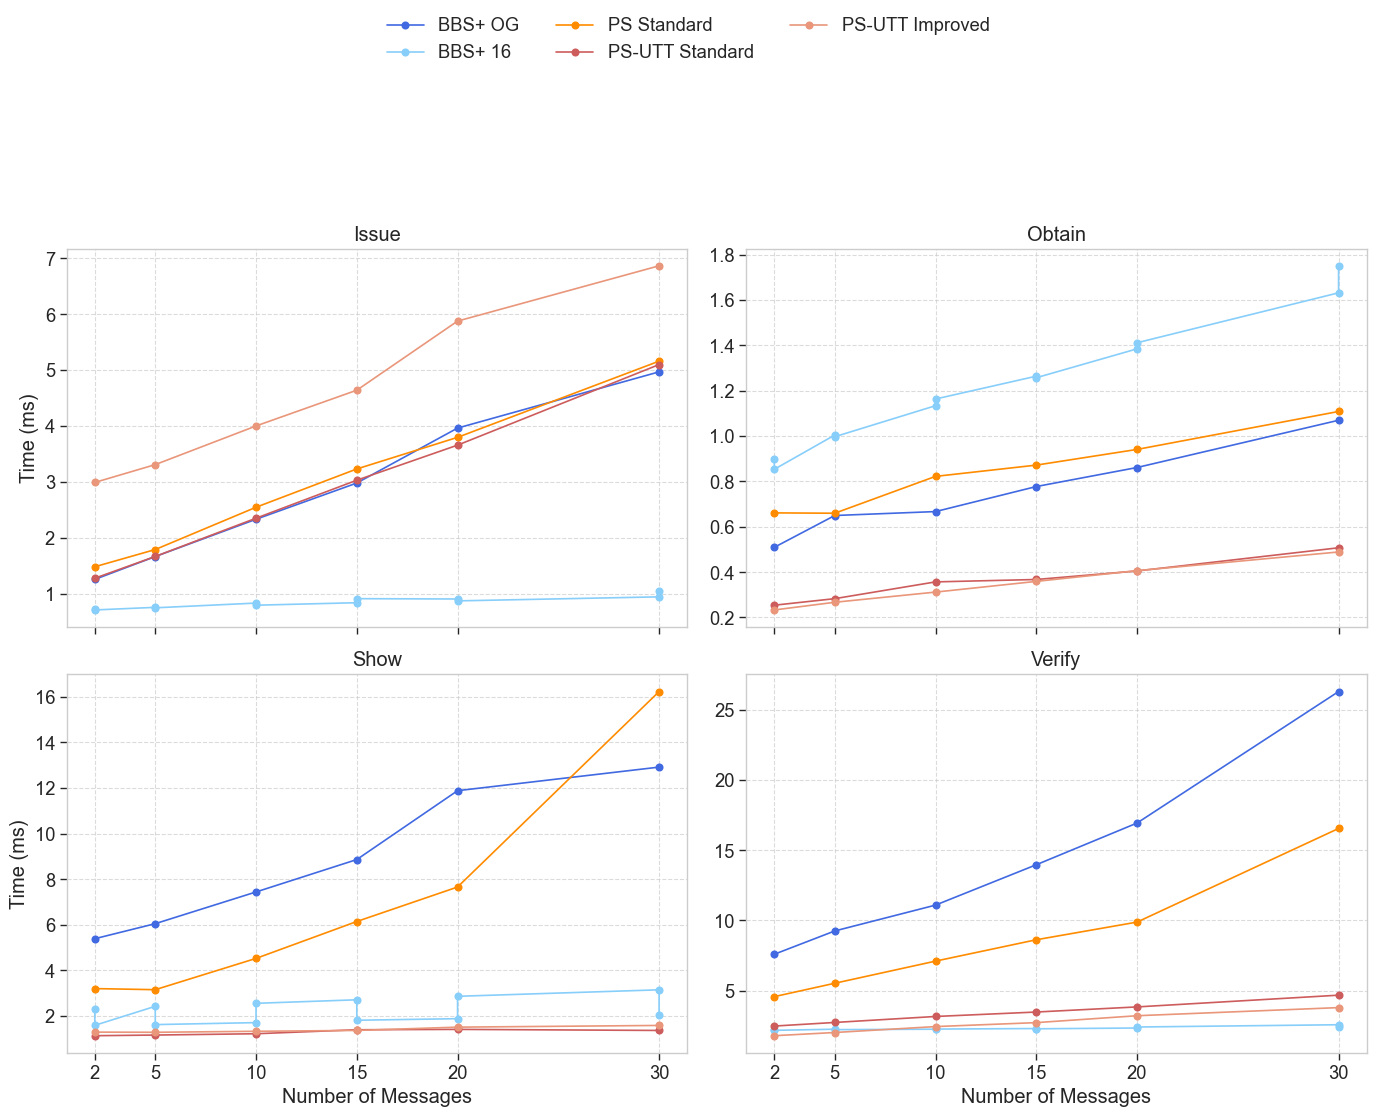
\includegraphics[width=1\linewidth]{comparison-line-graph.png}
    \caption{Performance Comparison of Anonymous Credential Schemes}
    
\end{figure}

\begin{figure}
    \centering
    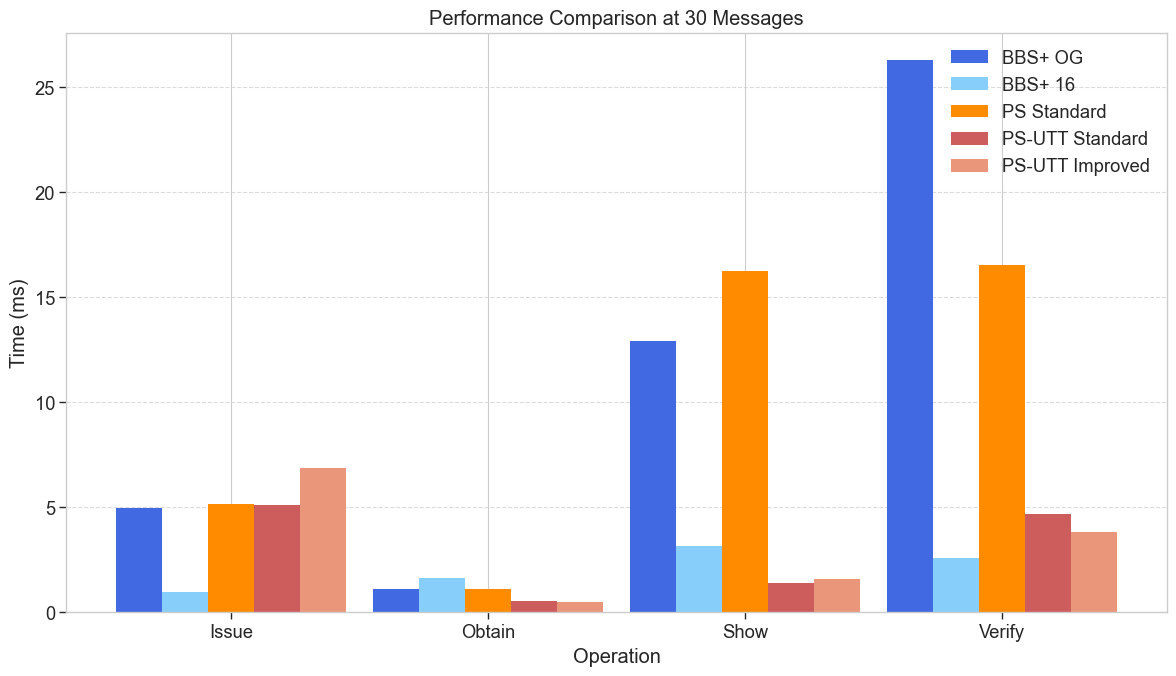
\includegraphics[width=0.7\linewidth]{performance-30.png}
    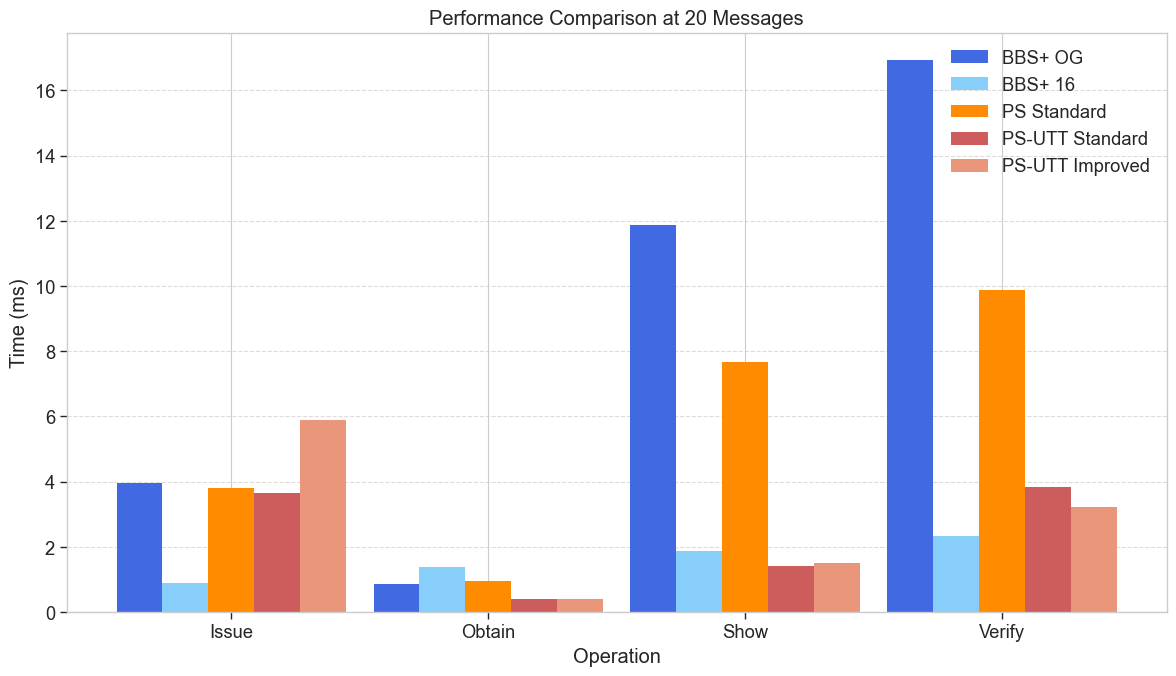
\includegraphics[width=0.7\linewidth]{performance-20.png}
    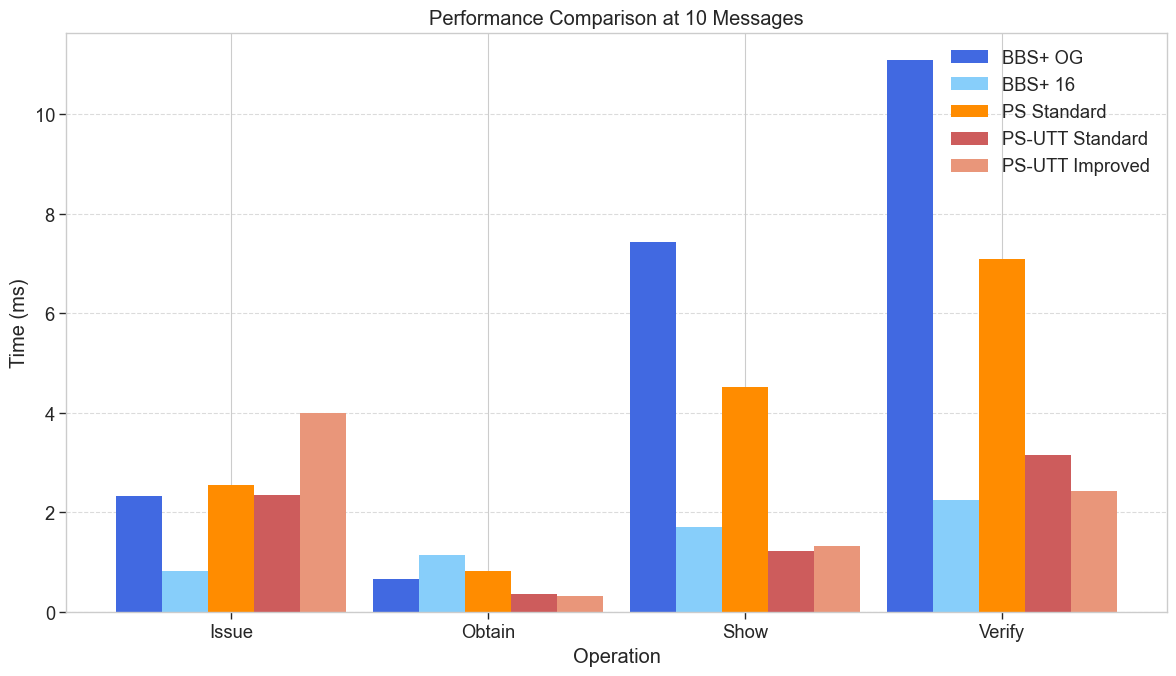
\includegraphics[width=0.7\linewidth]{performance-10.png}
     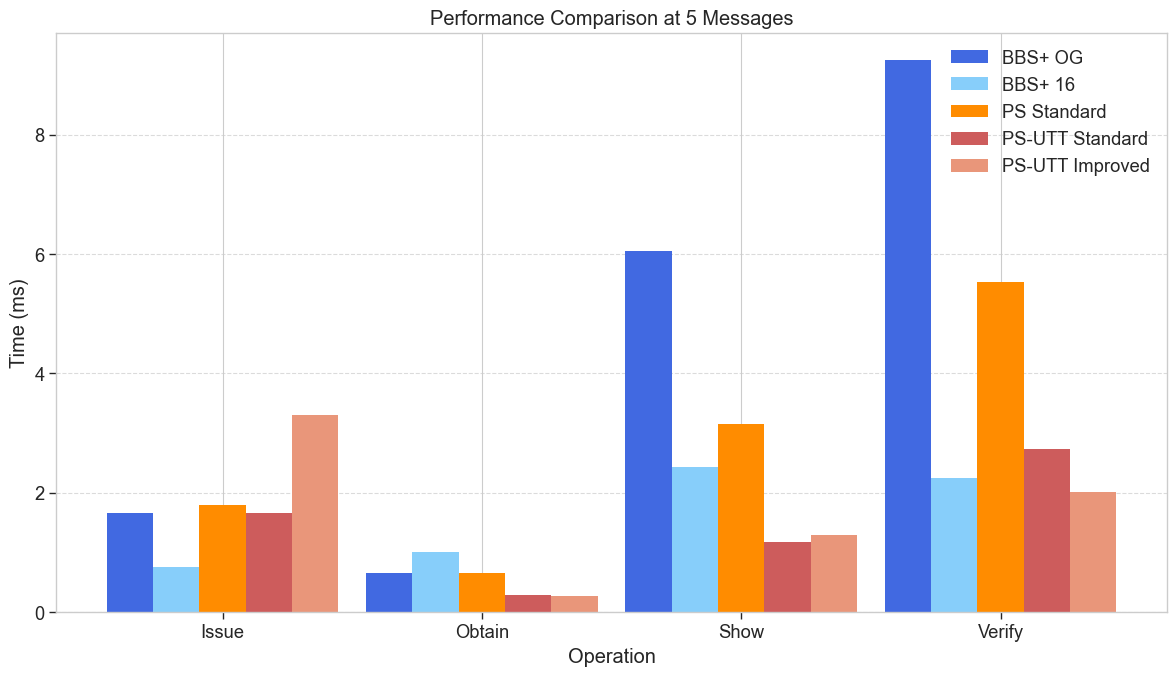
\includegraphics[width=0.7\linewidth]{performance-5.png}
    \caption{Performance Comparison of Anonymous Credential Schemes}
\end{figure}



\begin{table}[htbp]
\centering
\caption{Performance of Anonymous Credential Operations (time in ms)}
\begin{tabular}{@{}p{1.2cm}*{5}{>{\centering\arraybackslash}p{1.6cm}}@{}}
\toprule
n & BBS+ 06 & BBS+ 16 & PS 16 & PS-UTT G1 & PS-UTT G2 \\
\midrule
\multicolumn{6}{c}{\textbf{Obtain}}  \\
\midrule
\textbf{2} & 0.51 & 0.90 & 0.66 & 0.25 & \textbf{0.23} \\
\textbf{5} & 0.65 & 1.00 & 0.66 & 0.28 & \textbf{0.27} \\
\textbf{10} & 0.67 & 1.13 & 0.82 & 0.36 & \textbf{0.31} \\
\textbf{15} & 0.78 & 1.26 & 0.87 & 0.37 & \textbf{0.36} \\
\textbf{20} & 0.86 & 1.38 & 0.94 & \textbf{0.41} & 0.41 \\
\textbf{30} & 1.07 & 1.63 & 1.11 & 0.51 & \textbf{0.49} \\
\midrule
\multicolumn{6}{c}{\textbf{Issue}}  \\
\midrule
\textbf{2} & 1.25 & \textbf{0.72} & 1.48 & 1.27 & 2.99 \\
\textbf{5} & 1.66 & \textbf{0.75} & 1.79 & 1.66 & 3.31 \\
\textbf{10} & 2.33 & \textbf{0.83} & 2.54 & 2.35 & 4.00 \\
\textbf{15} & 2.98 & \textbf{0.84} & 3.23 & 3.03 & 4.64 \\
\textbf{20} & 3.96 & \textbf{0.90} & 3.79 & 3.66 & 5.88 \\
\textbf{30} & 4.97 & \textbf{0.94} & 5.16 & 5.10 & 6.86 \\
\midrule
\multicolumn{6}{c}{\textbf{Show}}  \\
\midrule
\textbf{2} & 5.39 & 2.31 & 3.20 & \textbf{1.14} & 1.29 \\
\textbf{5} & 6.05 & 2.42 & 3.15 & \textbf{1.16} & 1.29 \\
\textbf{10} & 7.44 & 1.71 & 4.53 & \textbf{1.22} & 1.33 \\
\textbf{15} & 8.86 & 2.71 & 6.14 & 1.40 & \textbf{1.37} \\
\textbf{20} & 11.88 & 1.88 & 7.66 & \textbf{1.41} & 1.51 \\
\textbf{30} & 12.91 & 3.15 & 16.23 & \textbf{1.37} & 1.59 \\
\midrule
\multicolumn{6}{c}{\textbf{Verify}}  \\
\midrule
\textbf{2} & 7.59 & 2.18 & 4.57 & 2.47 & \textbf{1.79} \\
\textbf{5} & 9.25 & 2.25 & 5.52 & 2.73 & \textbf{2.01} \\
\textbf{10} & 11.09 & \textbf{2.25} & 7.10 & 3.16 & 2.44 \\
\textbf{15} & 13.96 & \textbf{2.30} & 8.62 & 3.47 & 2.72 \\
\textbf{20} & 16.93 & \textbf{2.34} & 9.88 & 3.84 & 3.21 \\
\textbf{30} & 26.30 & \textbf{2.57} & 16.55 & 4.67 & 3.79 \\
\midrule
\multicolumn{6}{c}{\textbf{Issuing Phase Total (Obtain + Issue)}}  \\
\midrule
\textbf{2} & 1.76 & 1.62 & 2.14 & \textbf{1.53} & 3.22 \\
\textbf{5} & 2.31 & \textbf{1.76} & 2.45 & 1.95 & 3.57 \\
\textbf{10} & 3.00 & \textbf{1.96} & 3.37 & 2.71 & 4.31 \\
\textbf{15} & 3.75 & \textbf{2.10} & 4.10 & 3.40 & 5.00 \\
\textbf{20} & 4.82 & \textbf{2.29} & 4.74 & 4.06 & 6.28 \\
\textbf{30} & 6.04 & \textbf{2.57} & 6.27 & 5.60 & 7.35 \\
\midrule
\multicolumn{6}{c}{\textbf{Verify Phase Total (Show + Verify)}}  \\
\midrule
\textbf{2} & 12.98 & 4.48 & 7.77 & 3.61 & \textbf{3.08} \\
\textbf{5} & 15.30 & 4.67 & 8.68 & 3.90 & \textbf{3.30} \\
\textbf{10} & 18.53 & 3.96 & 11.62 & 4.38 & \textbf{3.77} \\
\textbf{15} & 22.82 & 5.01 & 14.76 & 4.87 & \textbf{4.09} \\
\textbf{20} & 28.81 & \textbf{4.22} & 17.53 & 5.25 & 4.72 \\
\textbf{30} & 39.21 & 5.72 & 32.77 & 6.04 & \textbf{5.37} \\
\bottomrule
\end{tabular}
\end{table}

















\section{Summary}
- Both PS and BBS+ anonymous credentials use pedersen commitment schemes and sigma protocols for proving knowledge of committed attributes
- PS benefits structurally, rerandomization is much cleaner, and with our variant, show + verify time is more efficient
- Proving knowledge of the committed attributes in PS and BBS+ delivers the Schnorr responses that can be used to prove identity binding - we actually get this for free with no extra cost
- Sigma proofs are the most efficient and expressive proofs for proving knowledge of committed attributes. Although theoretically, they are linear in the size of the attributes, they are still extraordinarily efficient. Practical efficiencies in cryptography libraries such as MSM and batch techniques such as window tables and parallel computation reduce the practical complexity to, in many cases, log of the committed attributes. Polynomial commitments such as in the case of SPS-EQ improve the theoretical complexity but reduce the expressiveness of the proofs, further analysis needs to be done to benchmark the practical comparison. 
- A users transaction with a 30 message anonymous credential (large but not impossible) will cost approximately 5.37ms which is considered efficient in transactions. 
- For proving knowledge of multiple credentials together, the schnorr protocol used in both BBS+ and PS outputs a mechanism (equality of responses) to verify the identifier in each credential and therefore, this almost comes for free. 









\section{Improvement Notes}
Notes for performance summary improvements

Conduct multi-credential benchmarks: Instead of just saying "verification produces Schnorr responses, we can use those to verify multiple credentials at the same time," actually measure and report the end-to-end time for verifying multiple credentials with identity binding. This is your main contribution and should be the centerpiece of your evaluation.

Add a cost breakdown: Include a small table or graph showing the time spent in each cryptographic operation (exponentiations, pairings, etc.) to demonstrate where your optimizations matter most.


Connect to application requirements: Briefly discuss what performance is needed for practical deployment (e.g., "authentication should complete in <100ms for acceptable user experience") and how your results meet these targets.

Implementation Approach
When conducting the multi-credential benchmarks, you might structure the experiment like this:

Measure end-to-end time for Show+Verify with 1, 2, 3, 4, and 5 credentials from different issuers
For each case, verify a predicate that requires identity binding across all credentials
Compare against a naive approach where each credential is verified independently
If possible, compare against TACT or another system that supports multi-credential verification





9.1 Experimental Methodology
We implemented our MIMC-ABC system using the arkworks library [citation] in Rust. All experiments were conducted on a MacBook Air M2 (2022) with 16GB RAM. Each measurement represents the average of 10 independent trials with standard deviations below 5%.
Our evaluation focuses on three key dimensions:

Single-credential efficiency: We compare the computational cost of basic operations (Obtain, Issue, Show, Verify) across five schemes: BBS+ (2006) [citation], BBS+ (2016) [citation], PS (2016) [citation], PS-UTT G1 [citation], and our optimized PS-UTT G2.
Multi-credential scalability: We measure end-to-end verification time when presenting multiple credentials from different issuers, comparing our system against alternative approaches.
Identity binding overhead: We evaluate the additional cost of our identity binding mechanism, which ensures multiple credentials belong to the same identity.

For attribute vectors, we use parameter n to represent the number of attributes in each credential (ranging from 2 to 30). For multi-credential scenarios, parameter m represents the number of distinct credentials being verified simultaneously (ranging from 1 to 5).

% https://claude.ai/chat/b60de4f9-f2a8-4640-85b3-bc87474dbf65
% 9.3 Multi-Credential Performance
% While single-credential performance is important, our system's key innovation is efficient verification of multiple credentials from different issuers. Figure 3 shows the end-to-end verification time (including both Show and Verify operations) as we increase the number of credentials presented simultaneously.
% We compared three approaches:

% Naive aggregation: Simply performing independent verification for each credential (linear scaling)
% TACT [citation]: A recent system supporting multi-credential presentation
% Our MIMC-ABC: Our system with optimized G2 signatures and identity binding

% As shown in Figure 3, our approach demonstrates significantly better scaling as the number of credentials increases. For a predicate requiring 5 credentials from different issuers, our system completes verification in just 12.4ms—a 3.2× improvement over the naive approach (39.7ms) and 1.8× faster than TACT (22.8ms).
% The efficiency stems from two key factors:

% Our G2 signature optimization reduces pairing operations per credential
% The Schnorr responses generated during Show protocol allow efficient identity binding verification with minimal additional overhead

% Figure 4 isolates this second factor by measuring the specific cost of identity binding across credentials. The additional verification time remains nearly constant (~1.1ms) regardless of the number of credentials being bound, demonstrating the efficiency of our approach to identity binding.

% 9.4 Analysis and Discussion
% Our performance evaluation reveals several key insights about the efficiency of MIMC-ABC:
% Single-Credential Performance Tradeoffs
% Table 1 shows that our G2 optimization significantly improves verification time (up to 28% faster than PS-UTT G1) at the cost of slightly increased issuing time. This tradeoff is well-justified for anonymous credential systems where credentials are issued once but verified many times.
% The performance profile of BBS+ (2016) deserves special mention—it achieves the fastest issuing times and competitive verification for large attribute counts. However, as we'll discuss below, it doesn't scale as efficiently for multi-credential scenarios due to limitations in its proof structure.
% Multi-Credential Efficiency
% The most significant advantage of our system emerges in multi-credential scenarios. Figure 3 demonstrates that MIMC-ABC's verification time grows much more slowly with additional credentials compared to alternative approaches. This is particularly important for complex verification policies that require multiple credentials from different issuers.
% Specifically, our system exhibits near-linear scaling in the number of attributes (n) but sub-linear scaling in the number of credentials (m), thanks to the efficient reuse of Schnorr responses across credential proofs. This aligns perfectly with real-world usage patterns where users may have many credentials but typically present a small subset (3-5) for any given verification.
% Practical Implications
% For a typical scenario involving 5 credentials with 10 attributes each, our system completes the entire Show+Verify process in under 15ms, which is well below the 100ms threshold typically considered acceptable for interactive user experiences. This makes MIMC-ABC suitable for deployment in performance-sensitive contexts like mobile authentication.
% The performance profile also allows us to recommend specific parameter choices for implementations:

% For mobile clients: Limit attribute count to n≤15 to keep Show operations under 2ms
% For verification servers: Up to m=10 credentials can be verified simultaneously while maintaining sub-50ms response times





% \begin{table}[h]
% \centering
% \begin{tabular}{|l|r|}
% \hline
% \textbf{Operation} & \textbf{Time} \\
% \hline
% Full Pairing & 1.6218 ms \\
% Miller Loop & 0.6931 ms \\
% Final Exponentiation & 0.9287 ms \\
% G1 Mixed Addition (Affine + Jacobian) & 672 ns \\
% G1 Point Doubling (2P) & 414 ns \\
% G2 Mixed Addition (Affine + Jacobian) & 2143 ns \\
% G2 Point Doubling (2P) & 1302 ns \\
% \hline
% Estimated G1 Scalar Mult (255-bit) & 191.59 $\mu$s \\
% \emph{\small(255 doublings + ~128 additions)} & \\
% Estimated G2 Scalar Mult (255-bit) & 606.01 $\mu$s \\
% \emph{\small(255 doublings + ~128 additions)} & \\
% \hline
% \end{tabular}
% \caption{Performance metrics for arkworks BLS12-381 implementation. Scalar multiplication estimates assume naive double-and-add implementation without optimizations.}
% \label{tab:arkworks-performance}
% \end{table}
% \footnotetext{The G1 and G2 scalar multiplication estimates are derived using a naive double-and-add implementation analysis for 255-bit scalars. For a random scalar $k$, we assume approximately 255 doubling operations (one per bit) and 128 addition operations (corresponding to an expected Hamming weight of $\frac{255}{2}$ for a random scalar). The G1 estimate of 191.59$\mu$s is computed as $(255 \times 414\text{ns}) + (128 \times 672\text{ns})$ using the measured doubling and mixed addition timings. Similarly, the G2 estimate of 606.01$\mu$s is computed as $(255 \times 1302\text{ns}) + (128 \times 2143\text{ns})$. These estimates represent upper bounds as they do not account for common optimizations such as windowing methods, NAF (Non-Adjacent Form) representations, or parallel computation strategies.}


\section{Identity Binding Results}

\subsubsection*{Experimental Setup}
Each scenario is tested across varying parameters ([4,16,32] credentials, [4,16,32] attributes per credential). We compare the non-private verification scenario against privacy-preserving verification to show the privacy overhead, we also include a comparison between single-issuer and multi-issuer to demonstrate that the multi-issuer environment is less efficient due to its inability to use batch verification because each verification key is different, but it's more flexible and required in certain use-cases like decentralized identity. All benchmarks use a fixed security parameter (BLS12-381 curve) and are executed on MacBook Air M2 16GB RAM on Sequoia 15.3.2. Results demonstrate the practical viability of privacy-preserving identity binding across multiple credential issuers in realistic authentication scenarios.

\subsection{Benchmarking Methodology}

Our benchmarking methodology focuses on evaluating the performance of identity binding across credentials, the core contribution of the MIMC-ABC system. We measure execution time specifically for credential show and verification scenarios, as these represent the critical path in authentication scenarios.

\begin{enumerate}
    \item \textbf{Non-private Mutli-Issuer verification (baseline)}: A user verifies their credential signatures and reveals identifiers in the clear. This establishes a performance baseline to quantify the overhead introduced by privacy-preserving techniques.

    \item \textbf{Non-private Single Issuer with Batch verification (baseline)}: A user verifies their credential signatures with batch verification and reveals identifiers in the clear. This establishes a performance baseline to quantify the overhead introduced by privacy-preserving techniques.

    \item \textbf{Private identity binding with multiple issuers}: The complete MIMC-ABC scenario where credentials from different issuers are presented with proofs of shared identity, demonstrating the system's full capability.

    \item \textbf{Private identity binding with single issuer}: Multiple credentials from the same issuer are presented with zero-knowledge proofs establishing shared identity, enabling batch verification optimizations for signatures from the same issuer.

\end{enumerate}

\subsection{The Privacy Overhead}

\begin{table}[ht]
\centering
\label{tab:single_issuer_performance}
\begin{tabular}{l@{\hspace{1.5em}}r@{\hspace{1.5em}}r@{\hspace{1.5em}}r}
\toprule
\multicolumn{4}{c}{\textbf{Single Issuer (Batch Verify)}} \\
\midrule
Credential Count & 4 & 16 & 32 \\
\midrule
Baseline Public Verify & 2.85 & 10.03 & 19.79 \\
Identity Binding (Private) Verify & 7.28 & 27.12 & 54.00 \\
Identity Binding (Private) Show + Verify & 12.28 & 47.35 & 94.10 \\
\bottomrule
\toprule
\multicolumn{4}{c}{\textbf{Multi Issuer}} \\
\midrule
Credential Count & 4 & 16 & 32 \\
\midrule
Baseline (Public) Verify & 6.77 & 27.69 & 54.31 \\
Identity Binding (Private) Verify & 18.67 & 76.52 & 148.24 \\
Identity Binding (Private) Show + Verify & 25.08 & 102.27 & 199.87 \\
\bottomrule
\end{tabular}
\caption{Single and Multi Issuer Performance Comparison (time in ms, 16 attributes per credential, Single-Issuer uses batch verification optimizations)}
\end{table}


\begin{figure}
    \centering
    % First row with two figures side by side
    \begin{minipage}{\textwidth}
        \centering
        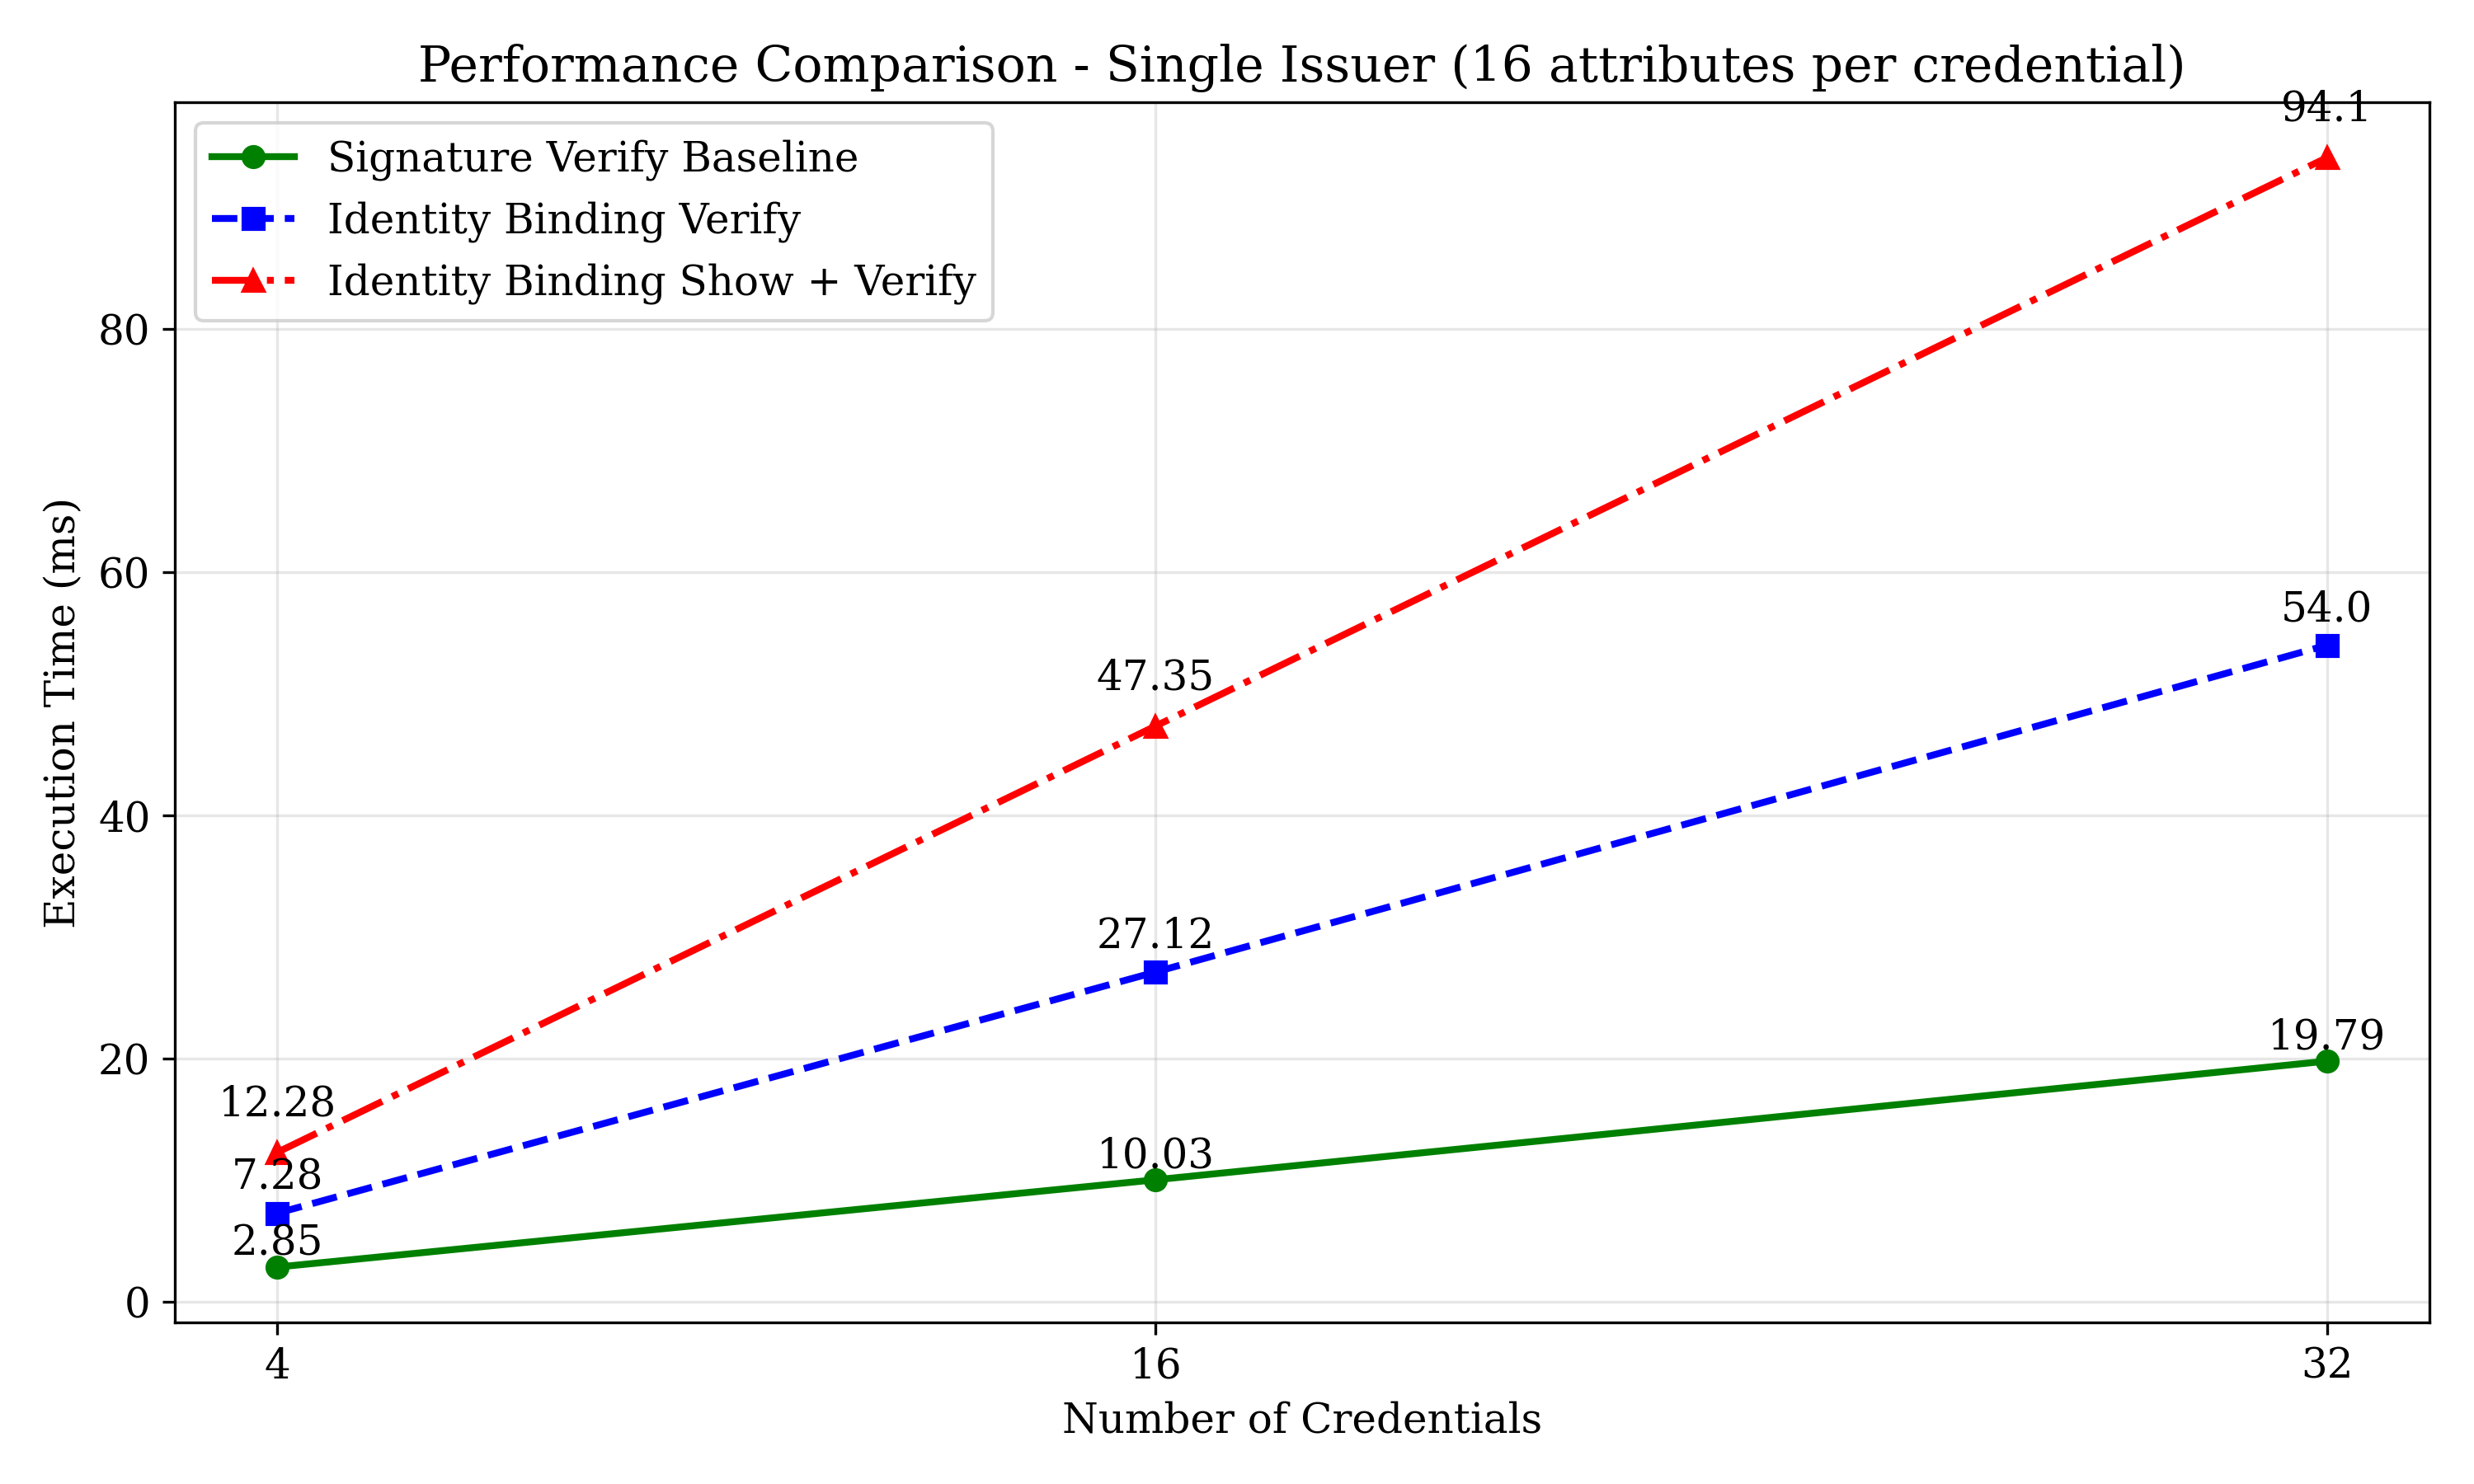
\includegraphics[width=0.48\textwidth]{figures/identity_binding_single_issuer_performance.png}
        \hfill
        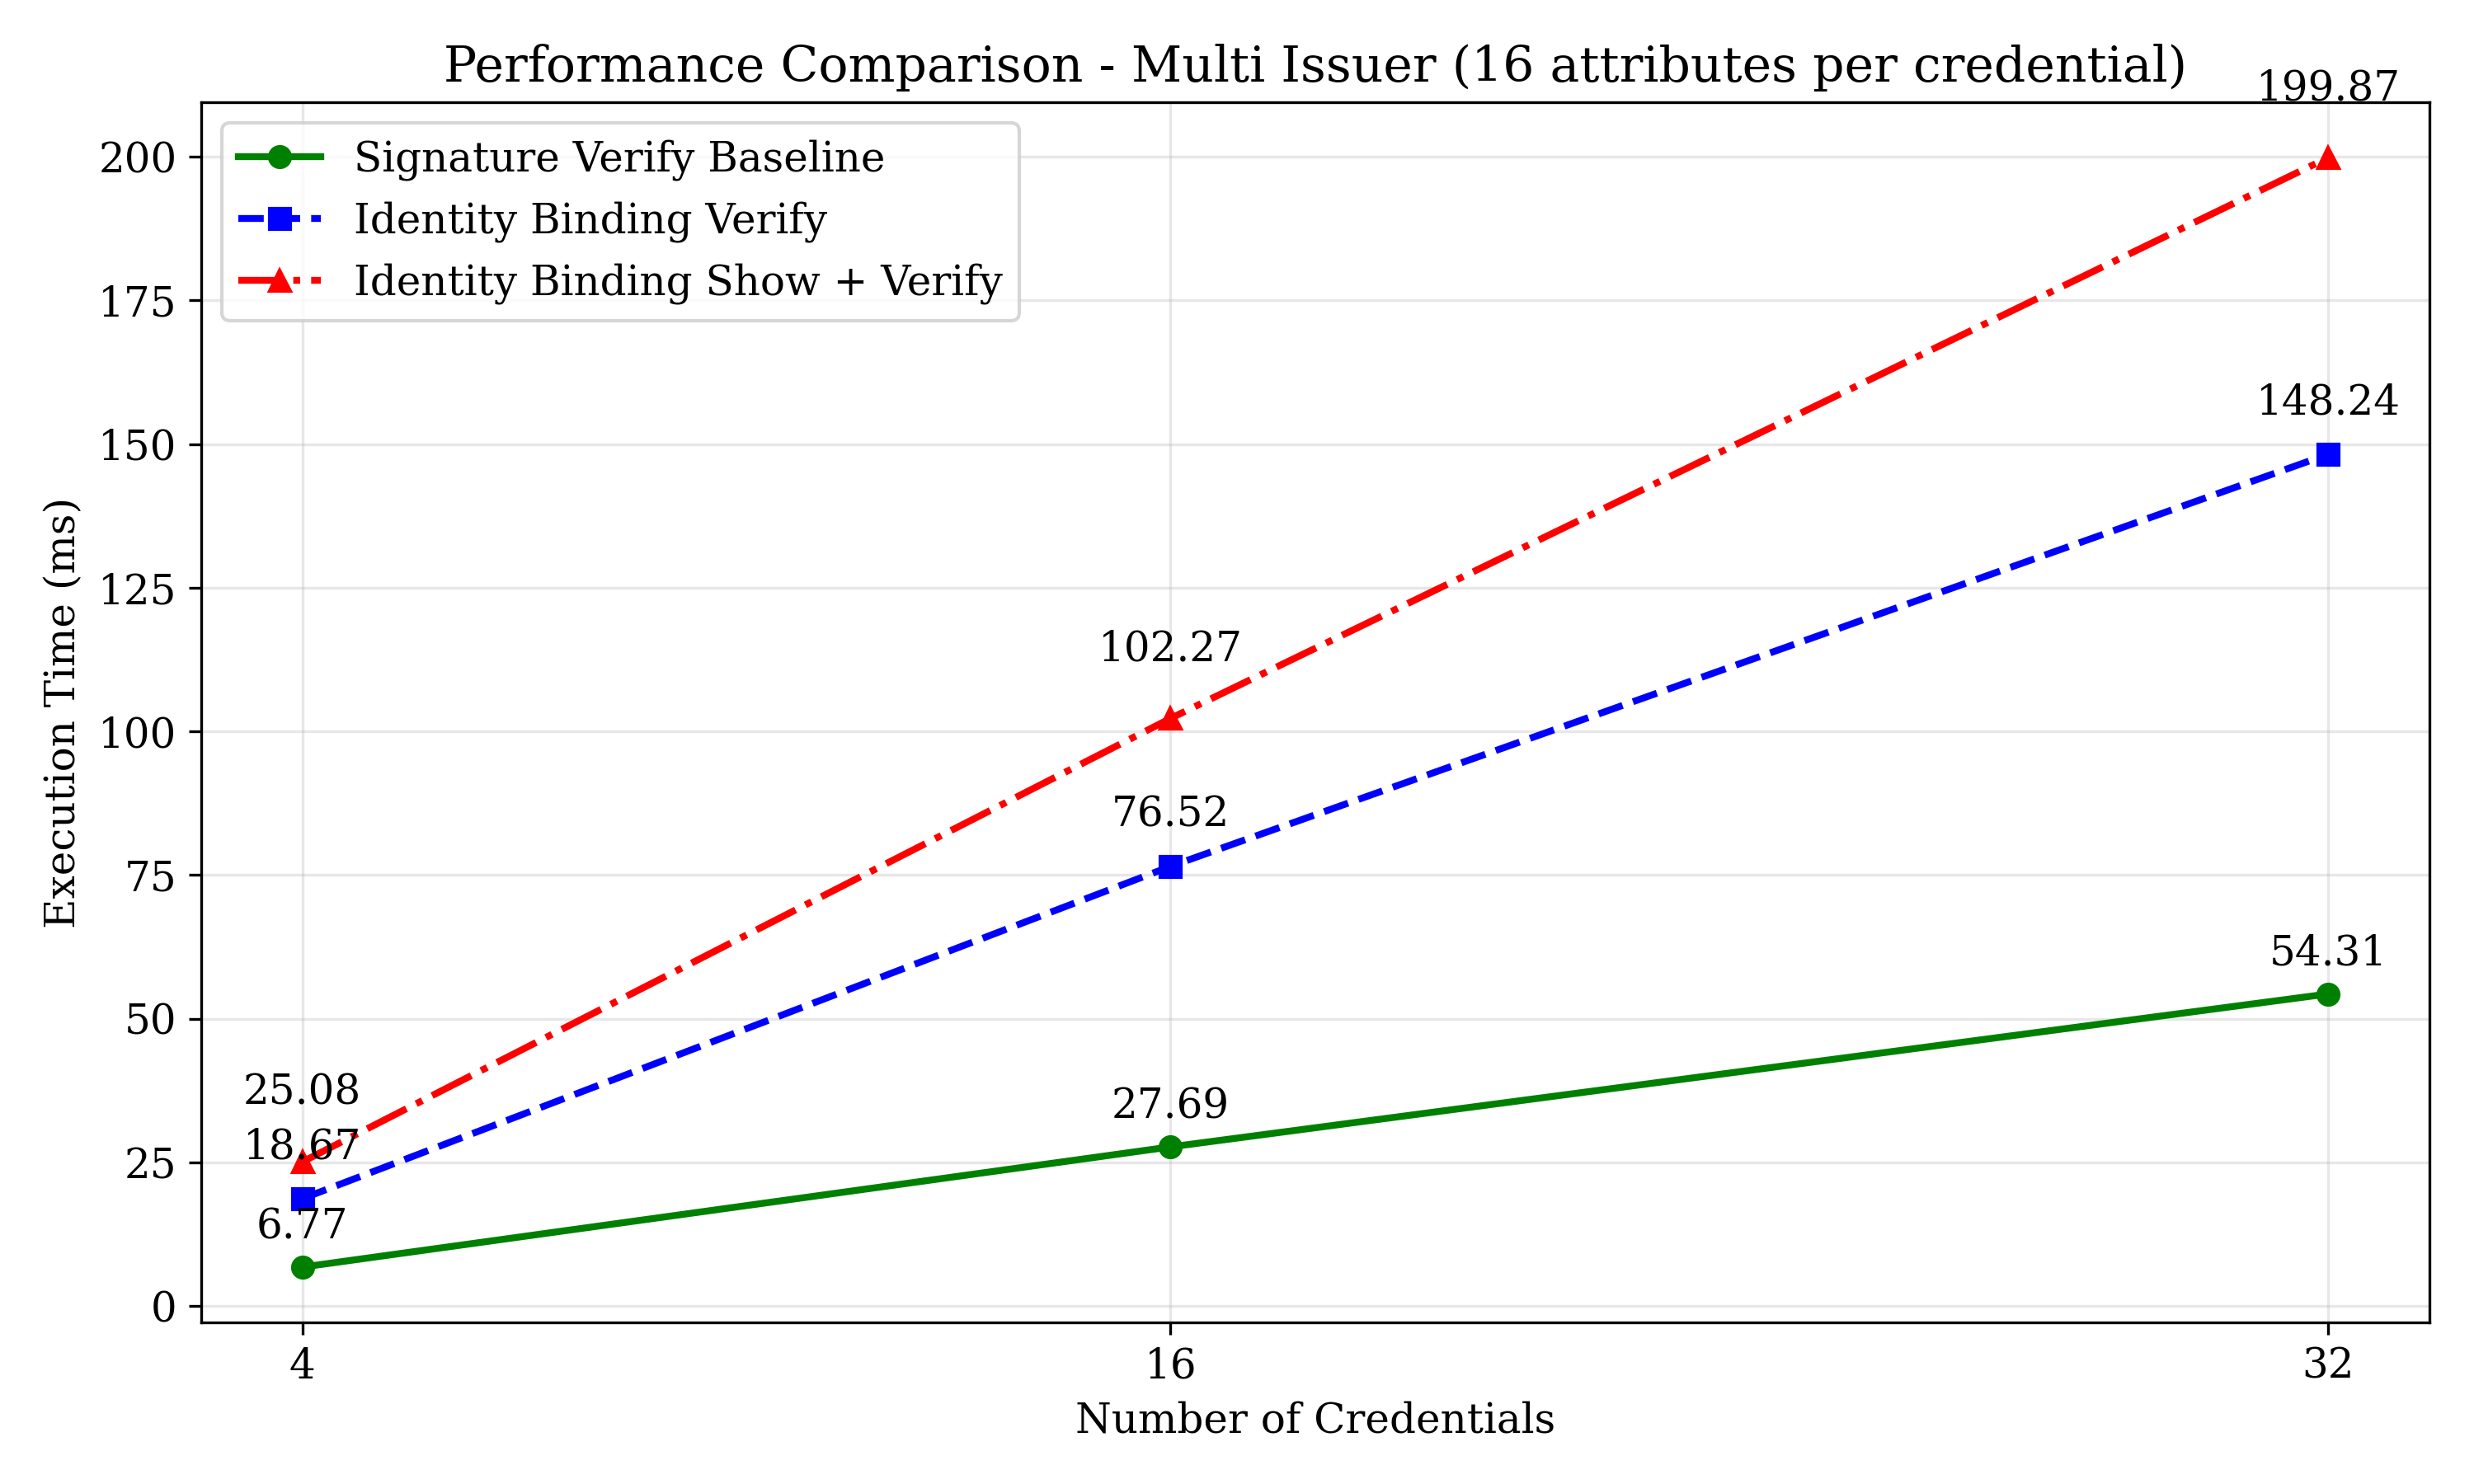
\includegraphics[width=0.48\textwidth]{figures/identity_binding_multi_issuer_performance.png}
    \end{minipage}
    
    \vspace{1em} % Add some vertical space between rows
    
    % Second row with one figure
    \begin{minipage}{\textwidth}
        \centering
        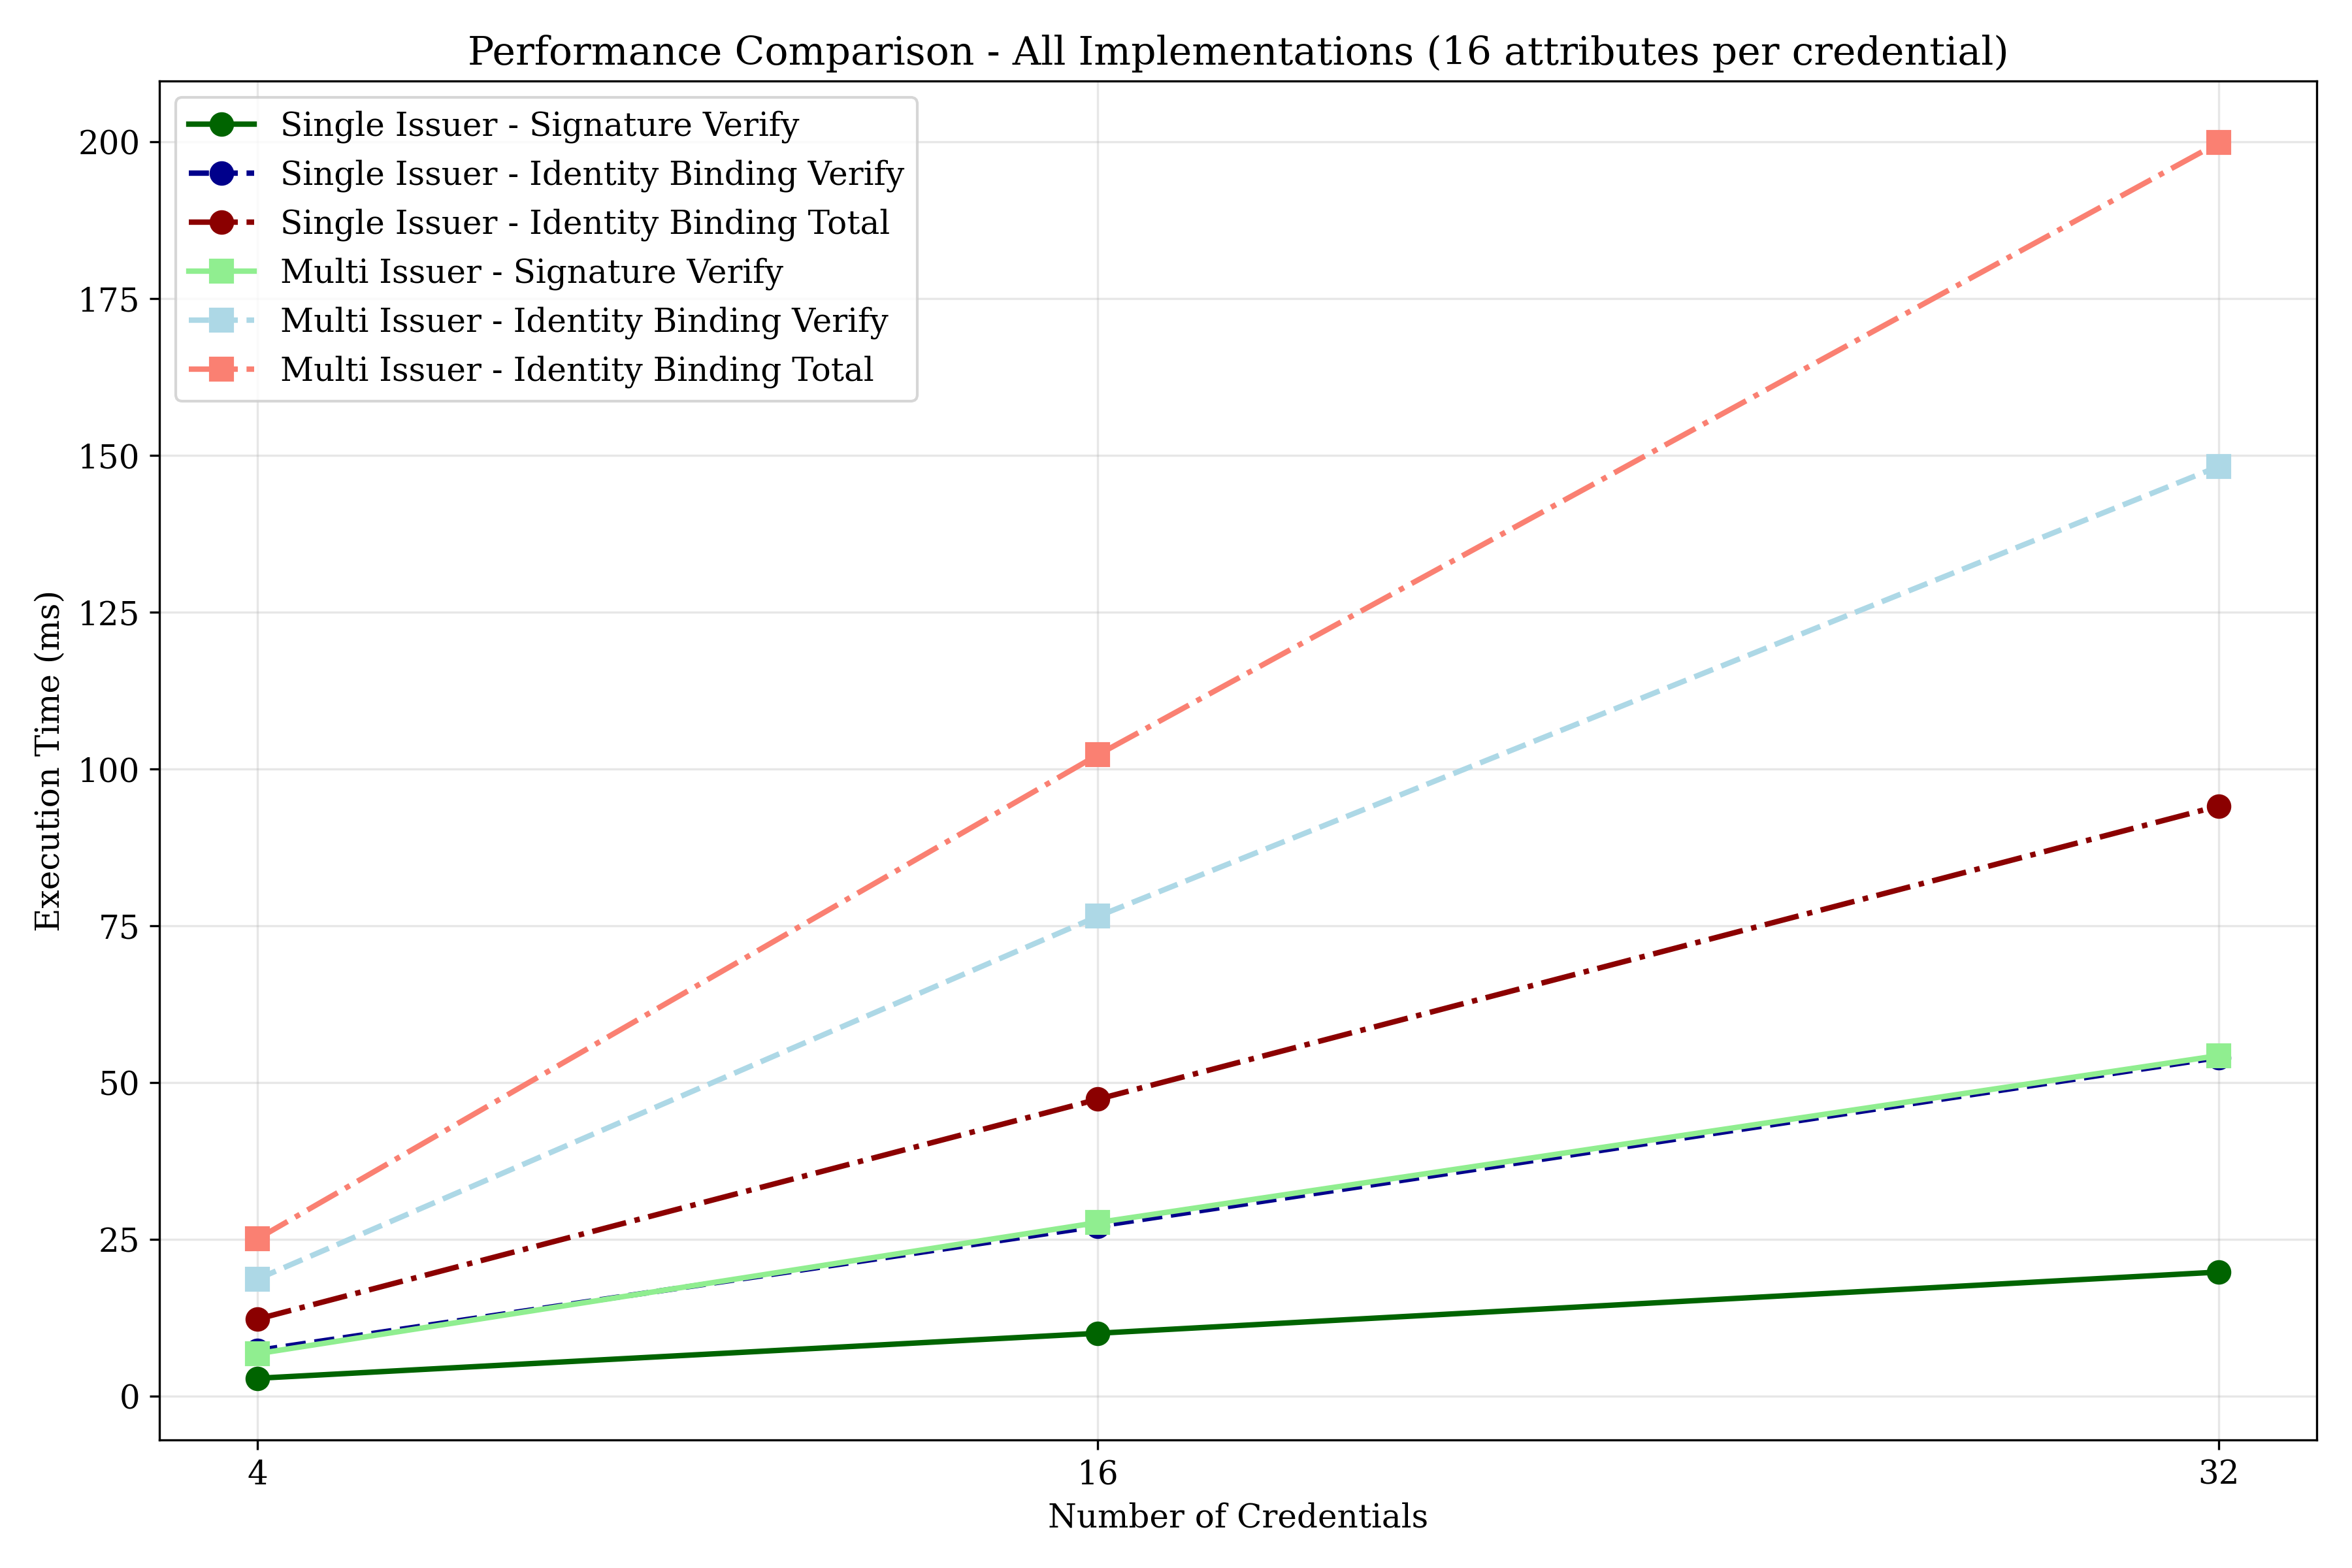
\includegraphics[width=0.48\textwidth]{figures/identity_binding_combined_performance.png}
    \end{minipage}
    
    \caption{Performance comparison between multi-issuer and single-issuer scenarios}
    \label{fig:performance-comparison}
\end{figure}
  \mychapter{}
  % start broad - the sybil resistance challenge in anonymous credential systems
% narrow to MIMC-ABC
% Introduce our solution
% Highlight our novelty

% Why = Motivation, Problem 
% How - what can be done to solve this problem
% Here's how we solved it and why we're better, what: it's a  Credential Relationship Bound Verifier from Pairing-Free VRF
\section{Credential Relationship Binding: Problem and Motivation}
In the $\MIMCABC$ system, identity binding ensures all credentials in a presentation belong to the same user by proving the equality of a committed identifier $\id$ across credentials. This enables users to prove multiple credentials together for application scenarios.
Credential Relationship binding extends this, enabling users to prove structured relationships between anonymous credentials, such as generating single-use tokens for integration with other systems e.g. privacy-pass-like applications \cite{davidson2018privacy} and for sybil-resistant context credentials.

Identity binding links credentials to a single user, credential relationship binding enforces dependency constraints between credentials, and a credential relationship bound nullifier is a deterministic anonymous token that proves the user has this relationship. Because it's determinisitic and based on the users secret attributes, they can only derive it in the same way, so the token is used for Sybil Resistance scenarios where privacy is still required and furthermore can be used in Revocation checks.

Sybil Resistance in private systems is difficult and furthermore in a multi-issuer, multi-credential scenario, simple relationship binding is not enough, as in $\MIMCABC$ a user can more easily maliciously create credentials with lower-security issuers that allow them to prove identity binding with attributes of their choice. 

\subsection{Limitation of existing approaches}
\begin{enumerate}
    \item \textbf{Standard VRF} computes a deterministic nullifier
    \[
        \nul \gets g^{1/(\key + \ctx)}    \qquad \nul \cdot (\pk)^{\ctx}
    \]
    
    where $\key$ is the secret key, $\pk = g^{\key}$ is the public key, and $\nul$ is verifiable by $\nul \cdot (\pk)^{\ctx}$ for a public $\ctx$. This does not preserve the anonymity notions required for Anonymous Credentials as $\pk$ is publicly used each usage
    \item \textbf{MPC PRF}: CanDID, a decentralized identity system, computes nullifiers from MPC PRF during credential issuance preserving anonymity properties with secure multiparty computation, which has large overhead, and because of the time spent during PRF generation, can't be used easily for other mechanisms like the output being in a revocation list.
    \item \textbf{Pairing-based VRF:}  We base our scheme on the notions in \cite{tomescu2022utt}, our novel contribution is its computation in $\G_1$ and thus removing the pairing computation and operation in $\G_2$, improving computation efficiency and allowing its use in non-pairing based schemes.
\end{enumerate}


\subsection{Credential Relationship Bound Verifier from Pairing-Free VRF}
\begin{itemize}
    \item VRF Overview: A Verifiable Random Function generates a pseudorandom, deterministic output nullifier 
    \[
    \nul \gets g^{1/(\key + \ctx)}
    \]
    Verifiable by a public key $\pk = g^{\key}$. In $\MIMCABC, \key$ is a committed attribute in a master credential and $\ctx$ is the unique identifier of the context credential

    \item Integration: Users commit $\key$ and $\ctx$ in Pedersen commitments e.g., $( \cm_k = g^{\key} h^r, \cm_{\ctx} = g^{\ctx} h^{r_2})$, compute the nullifier, and prove its correctness to the issuer using a zero-knowledge protocol. This ensures one nullifier per $(\key, \ctx)$ pair, preventing sybil attacks.
\end{itemize}


\subsection{Contributions}

\noindent We improve the state of the art by creating a lightweight VRF construction tailored for Anonymous Credential systems with 3 contributions:
\begin{enumerate}
        \item \textbf{Pairing-Free VRF in Prime-Order Groups:} We adapt the Dodis-Yampolskiy VRF structure to function efficiently in standard prime-order groups, achieving provable pseudorandomness under the $q$-Diffie-Hellman Inversion ($q$-DHI) assumption.

        \item \textbf{Zero-Knowledge Proof of Multiplicative Inverse:} We introduce a novel $\Sigma$-protocol that proves the multiplicative inverse relation between committed values $m_1 = k + \textsf{ctx}$ and $m_2 = 1/m_1$, we use it in our scheme to verify the correctness of the VRF nullifier without revealing user secrets. We show it generalizes naturally for similar requirements in $\Sigma$-protocols, especially those needing to prove the q-DHI.

         \item \textbf{Formal Security Guarantees:} We demonstrate sybil resistance reduces to the security of our construction, the unique provability of the vrf and the soundness of our $\Sigma$-protocol.
\end{enumerate}


\subsection{Related Work}
(explain where they're used, what construction, pros, cons, use-case) This might be what I need to benchmark against

UTT - Pairing based Verifiable Nullifier
CanDID - MPC PRF
tACT - 
Anonymous Counting Tokens: Verifiable Oblivious Pseudorandom function






Revocation: How does your nullifier support revocation checks? Mention this in 2.4.


\section{OLD WORK}








\newpage
\section{Sybil Resistant Anonymous Credentials}
Anonymous Credentials are employed in Identity Systems and Private Payment systems where the credential owner requires privacy, but the system requires resistance against Sybil Attacks. Privacy and Sybil Resistance are paradoxical in nature as privacy demands the system know as little about the credential as possible, and protecting against Sybil Resistance requires the system to be accountable for the credentials, for example, to prevent multiple credentials for the same attributes be issued, preventing system misuse. 

In non-private systems, a user with a credential would have a credential identifier representing the unique issuance of the credential to the user. Similarly, a cheque or bank transfer has an identifier associated with it to prevent fraudulent multi-time use. In privacy-based systems, nullifiers are used in the same context. Nullifiers are deterministic functions based on the credential or credential attributes that are used to improve privacy. For example, a nullifier generated from a credential can be used 

 Verifiable Random Functions (VRFs) offer a promising solution by enabling the generation of verifiably pseudorandom and deterministic nullifiers from user-specific information, suitable for presentation to an issuer or for revocation lists. Existing VRF-based schemes often rely on computationally intensive bilinear pairings or reveal user attributes, introducing overhead or privacy risks.



\noindent We improve the state of the art by creating a lightweight VRF construction tailored for Anonymous Credential systems with 3 contributions:
\begin{enumerate}
        \item \textbf{Pairing-Free VRF in Prime-Order Groups:} We adapt the Dodis-Yampolskiy VRF structure to function efficiently in standard prime-order groups, achieving provable pseudorandomness under the $q$-Diffie-Hellman Inversion ($q$-DHI) assumption.

        \item \textbf{Zero-Knowledge Proof of Multiplicative Inverse:} We introduce a novel $\Sigma$-protocol that proves the multiplicative inverse relation between committed values $m_1 = k + \textsf{ctx}$ and $m_2 = 1/m_1$, we use it in our scheme to verify the correctness of the VRF nullifier without revealing user secrets. We show it generalizes naturally for similar requirements in $\Sigma$-protocols, especially those needing to prove the q-DHI.

         \item \textbf{Formal Security Guarantees:} We demonstrate sybil resistance reduces to the security of our construction, the unique provability of the vrf and the soundness of our $\Sigma$-protocol.
\end{enumerate}
We first present the preliminaries and foundations of our VRF for committed inputs, the design of our $\Sigma$-protocol, and demonstrate how the integration achieves sybil resistance in anonymous credential systems.

\begin{definition}[Sybil-Resistant Issuance]
For any context $\ctx$, a Context Credential issuer must be able to detect if a user with master credential containing identifier $\id$ has previously obtained a context credential for $\ctx$, without learning $\id$ itself or linking this issuance request to other credential presentations.
\end{definition}

\subsection{Problem}
To understand how we use the VRF within our application, we introduce the application:
Within our anonymous credential system, a user has a Master Credential with a VRF key $k$ and Context Credential with $\textsf{ctx}$, where $\textsf{ctx}$ is the context, such as $\mathcal{H}(\textit{"DriversLicense"})$ where $\mathcal{H}$ is hashes a string to $\Z_p$
\[
\cm_{\textsf{m}} = \mathsf{CM.Com}([k, \ldots]; r) = g_1^{k}\ldots h^r \quad \wedge \quad \cm_{\textsf{c}} = \mathsf{CM.Com}([\textsf{ctx}, \ldots]; r_2) = g_1^{\textsf{ctx}} \ldots h^{r_2}
\]
During Context Credential issuance, a user must prove to the issuer that their context credential hasn't been issued before, that is, the Context Credential issuance must be \emph{Sybil Resistant}. Our goal is to generate a unique, unlinkable nullifier for a specific context containing something in both the Master Credential and the Context Credential to protect the system from Sybil attacks while also retaining user privacy.

We leverage the structure and properties of the Dodis Yampolisky Verifiable Random Function (VRF)
\[
\text{Nullifier } \textsf{N} = g^{1/k + \textsf{ctx}}
\]

The Nullifier takes on the properties of correctness, pseudorandomness, and provable uniqueness from the VRF which we exploit in our protocol.


\subsection{Preliminaries}

\begin{definition}[q-DHI Assumption]
Let $\mathbb{G}$ be a cyclic group of prime order $p$ with generator $g$. The $q$-Diffie-Hellman Inversion ($q$-DHI) assumption \cite{mitsunari_new_2002} states that for any PPT adversary $\mathcal{A}$, there exists a negligible function $\negl$ such that:
\[
\Pr\left[ x \sample \Zp^*, \quad \mathcal{A}(g, g^x, g^{x^2}, \ldots, g^{x^q}) = g^{1/x} \right] \leq \negl 
\]
where the probability is taken over the random choice of $x$ and the random coins of $\mathcal{A}$. Informally, no $\PPT$ adversary can distinguish between $g^{1/\alpha}$ from a random group element.
\end{definition}

\begin{remark}
The $q$-DHI assumption is equivalent to the $(q+1)$-generalized Diffie-Hellman assumption (GDH) as shown by Boneh and Boyen \cite{kanade_efficient_2004}. This equivalence provides a solid theoretical foundation for our VRF construction's security.
\end{remark}




\begin{definition}[Verifiable Random Function in Prime-Order Group]
A Verifiable Random Function (VRF) in prime-order group $\G$ of order $q$ is a tuple of PPT algorithms $(\mathsf{VRF.Gen}, \mathsf{VRF.Eval}, \mathsf{VRF.Vfy})$ with associated message space $\setX$, output space $\setN$, and proof space $\Pi$, defined as:

\begin{itemize}
    \item $\mathsf{VRF.Gen}(1^\lambda) \to (sk, pk):$ Samples secret key $\alpha \sample \Zp^*$, computes public key $pk \gets g^\alpha$, returns $(sk = \alpha, pk)$
    
    \item $\mathsf{VRF.Eval}(sk, x) \to \textsf{N}, \pi:$ Returns output $\textsf{N} \gets g^{1/(x+sk)}$ and $\pi$ verifies the output $\textsf{N}$
    
    \item $\mathsf{VRF.Vfy}(pk, x, \textsf{N}, \pi) \to \bit:$ validates proof $\pi$ that $\textsf{N} = g^{1/(x+sk)}$, outputs 1 for success, 0 for failure
\end{itemize}
\end{definition}

\begin{itemize}
    \item \textbf{Correctness:} For all $(sk, pk) \gets \mathsf{VRF.Gen}(1^\lambda)$ and all $x \in \setX$:
    \[
    \Pr\left[\begin{aligned}
        (y, \pi) &\gets \mathsf{VRF.Eval}(sk, x) \\
        1 &\gets \mathsf{VRF.Vfy}(pk, x, \textsf{N}, \pi)
    \end{aligned}\right] = 1
    \]

    \item \textbf{Unique Provability:} For any $pk$ (possibly malicious) and $x \in \setX$, no $\PPT$ adversary $\AdvA$ can find two distinct pairs of outputs $(\textsf{N}_0, \pi_0) \neq (\textsf{N}_1, \pi_1)$ such that:
    \[
    \mathsf{VRF.Vfy}(pk, x, \textsf{N}_0, \pi_0) = \mathsf{VRF.Vfy}(pk, x, \textsf{N}_1, \pi_1) = 1
    \]

    \item \textbf{Pseudorandomness:} For every PPT adversary $\AdvA$, there exists negligible function $\negl$ such that:
    \[
    \left|\Pr\left[\mathsf{Exp}_{\mathsf{VRF}}^{\mathsf{PR}}(\AdvA, \lambda) = 1\right] - \frac{1}{2}\right| \leq \negl
    \]
    where the pseudorandomness experiment $\mathsf{Exp}_{\mathsf{VRF}}^{\mathsf{PR}}$ is defined in the standard framework for VRFs.
\end{itemize}


\subsection{Algebraic Analysis of Dodis Yampolskiy VRF}
We first recall the classical Dodis Yampolskiy VRF construction with bilinear pairings, we demonstrate with Type-3 pairings as they are generally used in practice. Let $\G_1, \G_2, \G_T$ be groups of a bilinear map with prime order $p$ where $g_1, g_2$ are generators for $\G_1, \G_2$ respectively and $e$ is an efficient map from $\G_1 \times \G_2 \to \G_T$:

% \begin{itemize}
%     \item $\mathsf{VRF.Gen}(\secparam)$: Samples $k \sample \Z_p$, set $pk = g^k$ 
    
%     \item $\mathsf{VRF.Eval}(k, \ctx) \to $(\mathsf{N}, \pi)$: $\pi = e(g_1, g_2)^{1/(k + \textsf{ctx})}$, $\mathsf{N} = g_2^{1/(k + \textsf{ctx})}$ 
    
%     \item $\mathsf{VRF.Vfy}(pk, \textsf{ctx}, \mathsf{N}, \pi) \to \bit$: assert $\quad$ $e(g^{\textsf{ctx}} \cdot pk, \mathsf{N})  \stackrel{?}{=} e(g_1, g_2) \quad \wedge \quad \pi  \stackrel{?}{=} e(g_1, \mathsf{N})$
% \end{itemize}

$\mathsf{Eval}$ computes the nullifier $\textsf{N}$ and generates a proof $\pi$ to prove that anyone in possession of $pk$ and the input $\textsf{ctx}$ can verify $\textsf{N}$ was computed correctly. $\mathsf{Vfy}$ resembles a signature verification as it binds  the public key $pk$, input $\textsf{ctx}$, and nullifier output together. 

The first pairing binds the public input $pk, \mathsf{ctx}$ with $\mathsf{N}$
\begin{align*}
    e(g_1^\mathsf{ctx} \cdot pk, \mathsf{N})  \quad  \stackrel{?}{=}& \quad  e(g_1, g_2) \\
    e(g_1^\mathsf{ctx}, g_2^{1/(k + \mathsf{ctx})}) \cdot  e(pk, g_2^{1/(k + \mathsf{ctx})}) \quad  \stackrel{?}{=}& \quad  e(g_1, g_2) \\
    e(g_1^\mathsf{ctx}, g_2)^{1/(k + \mathsf{ctx})} \cdot  e(g_1^k, g_2)^{1/(k + \mathsf{ctx})} \quad  \stackrel{?}{=}& \quad  e(g_1, g_2) \\
    e(g_1, g_2)^{\mathsf{ctx}/(k + \mathsf{ctx})} \cdot  e(g_1^k, g_2)^{k/(k + \mathsf{ctx})} \quad  \stackrel{?}{=}& \quad  e(g_1, g_2) \\
    e(g_1, g_2)^{\mathsf{ctx} + k/(k + \mathsf{ctx})}  \quad =& \quad e(g_1, g_2) \\
\end{align*}

\begin{align*}
     \pi  \quad  \stackrel{?}{=}& \quad e(g_1, \mathsf{N}) \\
     e(g_1, g_2)^{1/(k + \textsf{ctx})}  \stackrel{?}{=}& \quad  e(g_1, g_2^{1/(k + \mathsf{ctx})}) \\
     e(g_1, g_2)^{1/(k + \textsf{ctx})}  \stackrel{?}{=}& \quad  e(g_1, g_2)^{1/(k + \textsf{ctx})} \\
\end{align*}

% And the second pairing binds the proof $\pi$ to \mathsf{N}$

\subsubsection{Informal Security analysis of Bilinear Pairing VRF}
\begin{itemize}
    \item \textbf{Correctness:} Follows directly from pairing properties. The algebraic structure ensures verification equations hold when computed honestly.
    
    \item \textbf{Unique Provability:} Each nullifier $\mathsf{N} = g_2^{1/(k+\textsf{ctx})}$ is uniquely determined by the pairing equation $e(g_1^{k + \textsf{ctx}}, \mathsf{N}) = e(g_1, g_2)$. A forgery requires solving DLOG to create  $g_2^{1/(k+\textsf{ctx}')} = \mathsf{N}$.
    
    \item \textbf{Pseudorandomness:} Relies on the $q$-DHI assumption in bilinear groups. Given $g_1, g_1^k, g_1^{k^2}, \ldots$, distinguishing $\mathsf{N} = g_2^{1/(k+\textsf{ctx})}$ from random reduces to computing $g_2^{1/k}$ (a $q$-DHI instance).
\end{itemize}



\subsection{VRF with Committed Inputs}
As demonstrated above, the classical Dodis-Yampolskiy VRF uses pairings to verify the relationship between inputs and outputs through the equation: $e(g_1^{\textsf{ctx}} \cdot pk, \mathsf{N}) = e(g_1, g_2)$. Our key insight is that this pairing equation fundamentally verifies a multiplicative relationship. When we expand the left side: $e(g_1^{\textsf{ctx}} \cdot g_1^k, g_2^{1/(k + \textsf{ctx})}) = e(g_1, g_2)$ we are effectively proving that $(k + \textsf{ctx}) \cdot \frac{1}{k + \textsf{ctx}} = 1$. 

This observation suggests an alternative approach: instead of using pairings to verify this relationship, we can prove it directly through a carefully constructed $\Sigma$-protocol. Let:
\begin{itemize}
    \item $m_1 = k + \textsf{ctx}$ (committed in $\cm_1$)
    \item $m_2 = \frac{1}{k + \textsf{ctx}}$ (committed in $\cm_2$)
\end{itemize}

The VRF nullifier is then simply $\mathsf{N} = g^{m_2}$, and verification reduces to proving:
\begin{enumerate}
    \item $m_1$ is correctly formed from committed values $k$ and $\textsf{ctx}$
    \item $m_1 \cdot m_2 = 1$ (multiplicative inverse relation)
    \item $\mathsf{N} = g^{m_2}$ (nullifier structure)
\end{enumerate}

This reformulation eliminates the need for pairings while maintaining the security properties of the original VRF. The challenge now becomes constructing an efficient $\Sigma$-protocol that proves these relationships without revealing the underlying values.



\subsection{Commitment Structure for VRF Verification}
To privately prove the VRF relationship, we commit to both the input relationship and multiplicative inverse:

% \begin{itemize}
%     \item Primary commitments to inputs:
%         \[\cm_k = g^k h^{r_1}, \quad \cm_{\textsf{ctx}} = g^{\textsf{ctx}} h^{r_2}\]
    
%     \item Derived commitment to their sum:
%         \[\cm_3 = \cm_k^{\textsf{ctx}} h^{r_3}
    
%     \item Commitment to the inverse:
%         \[\cm_4 = \cm^{m_2} h^{r_4} \text{ where } m_2 = \frac{1}{m_1}\]
% \end{itemize}

The algebraic structure of these commitments enables our $\Sigma$-protocol to efficiently prove the multiplicative inverse relationship while maintaining zero-knowledge.


\subsection{Sigma-Protocol Construction}
Given these commitments, we construct a $\Sigma$-protocol that proves the VRF relationship in zero-knowledge. The protocol leverages auxiliary commitments $\cm_3, \cm_4$
to enforce the multiplicative inverse relationship: $\Pi^{\mathcal{R}_{\textsf{VRF}}}$ from 

    \[
        \mathcal{R}_{\mathsf{vrf}} = \left\{ (\cm_k, \cm_{\textsf{ctx}}, \mathsf{N}), (k, \textsf{ctx}, r_1, r_2) \; \Big| \;  \cm_k = g^k h^{r_1} \; \land \;
                \cm_{\textsf{ctx}} = g^{\textsf{ctx}} h^{r_2} \land \textsf{N} = g^{1/(k + \textsf{ctx})} \right\}
    \]



\newpage
\begin{protocol}{VRF Output Verification}{vrf-verify}\label{pok-vrf}
\textbf{Common Input:} Commitments $\cm_1, \cm_2$, group generator $g$, and public parameters $h \in \G$\\
\textbf{Prover Input:} Witness $(m_1, m_2, r_1, r_2, r_3, r_4)$ such that:
\begin{itemize}
    \item $\cm_1 = g^{m_1}h^{r_1}$ and $\cm_2 = g^{m_2}h^{r_2}$
    \item $\cm_3 = \cm_1^{m_2}h^{r_3}$ and $\cm_4 = h^{r_4}$
    \item $m_1 \cdot m_2 = 1$ (multiplicative inverse relation)
\end{itemize}

\begin{enumerate}
    \item \textbf{Commitment:} Prover samples randomness:
    \[
        \alpha_1, \alpha_2, \rho_1, \rho_2, \rho_3, \rho_4 \sample \Z_q
    \]
    Computes:
    \begin{itemize}
        \item $T_1 \gets g^{\alpha_1}h^{\rho_1}$
        \item $T_2 \gets g^{\alpha_2}h^{\rho_2}$
        \item $T_3 \gets \cm_1^{\alpha_2}h^{\rho_3}$
        \item $T_4 \gets h^{\rho_4}$
    \end{itemize}
    Sends $(T_1, T_2, T_3, T_4)$ to verifier.
    
    \item \textbf{Challenge:} Verifier samples $c \sample \Z_q$ and sends to prover.
    
    \item \textbf{Response:} Prover computes:
    \begin{align*}
        s_1 &\gets \alpha_1 + c \cdot m_1 &u_1 &\gets \rho_1 + c \cdot r_1\\
        s_2 &\gets \alpha_2 + c \cdot m_2 &u_2 &\gets \rho_2 + c \cdot r_2\\
        u_3 &\gets \rho_3 + c \cdot r_3 &u_4 &\gets \rho_4 + c \cdot r_4
    \end{align*}
    Sends $(s_1, s_2, u_1, u_2, u_3, u_4)$ to verifier.
    
    \item \textbf{Verification:} Verifier checks:
    \begin{enumerate}[label=(\roman*)]
        \item $g^{s_1}h^{u_1} \stackrel{?}{=} T_1 \cdot \cm_1^c$
        \item $g^{s_2}h^{u_2} \stackrel{?}{=} T_2 \cdot \cm_2^c$
        \item $\cm_1^{s_2}h^{u_3} \stackrel{?}{=} T_3 \cdot \cm_3^c$
        \item $h^{u_4} \stackrel{?}{=} T_4 \cdot \cm_4^c$
        \item $\frac{\cm_3}{\cm_4} \stackrel{?}{=} g$
    \end{enumerate}
\end{enumerate}
\end{protocol}

\paragraph{Security Analysis:}
The protocol satisfies the following security properties:

\begin{itemize}
    \item \textbf{Completeness:} For honest prover and verifier, all verification equations hold algebraically:
    \begin{align*}
        g^{s_1}h^{u_1} &= g^{\alpha_1 + cm_1}h^{\rho_1 + cr_1} = T_1 \cdot \cm_1^c\\
        g^{s_2}h^{u_2} &= g^{\alpha_2 + cm_2}h^{\rho_2 + cr_2} = T_2 \cdot \cm_2^c\\
        \cm_1^{s_2}h^{u_3} &= \cm_1^{\alpha_2 + cm_2}h^{\rho_3 + cr_3} = T_3 \cdot \cm_3^c\\
        h^{u_4} &= h^{\rho_4 + cr_4} = T_4 \cdot \cm_4^c
    \end{align*}
    
    \item \textbf{Special Soundness:} Given two accepting transcripts $(T_1, T_2, T_3, T_4, c, s_1, s_2, u_1, u_2, u_3, u_4)$ and $(T_1, T_2, T_3, T_4, c', s_1', s_2', u_1', u_2', u_3', u_4')$ with $c \neq c'$, the extractor $\mathcal{E}$ works as follows:
    \begin{align*}
        m_1 &= \frac{s_1 - s_1'}{c - c'} &r_1 &= \frac{u_1 - u_1'}{c - c'}\\
        m_2 &= \frac{s_2 - s_2'}{c - c'} &r_2 &= \frac{u_2 - u_2'}{c - c'}\\
        r_3 &= \frac{u_3 - u_3'}{c - c'} &r_4 &= \frac{u_4 - u_4'}{c - c'}
    \end{align*}
    The extracted witness satisfies all verification equations and the multiplicative inverse relation by the binding property of Pedersen commitments.
    
    \item \textbf{Honest-Verifier Zero-Knowledge:} The simulator $\mathcal{S}$ operates as follows:
    \begin{enumerate}
        \item Sample $s_1, s_2, u_1, u_2, u_3, u_4 \sample \Z_q$ uniformly
        \item Compute simulated commitments:
        \begin{align*}
            T_1 &\gets g^{s_1}h^{u_1} \cdot \cm_1^{-c}\\
            T_2 &\gets g^{s_2}h^{u_2} \cdot \cm_2^{-c}\\
            T_3 &\gets \cm_1^{s_2}h^{u_3} \cdot \cm_3^{-c}\\
            T_4 &\gets h^{u_4} \cdot \cm_4^{-c}
        \end{align*}
        \item Output $(T_1, T_2, T_3, T_4, c, s_1, s_2, u_1, u_2, u_3, u_4)$
    \end{enumerate}
    The simulated transcript is perfectly indistinguishable from a real transcript as the distribution of responses $(s_1, s_2, u_1, u_2, u_3, u_4)$ is uniform in both cases, and the commitments are uniquely determined by the verification equations.
\end{itemize}

\paragraph{Connection to VRF Security}  
The protocol’s soundness guarantees that $\textsf{N} = g^{m_2}$ is valid only if $m_2 = 1/m_1$ for $m_1 = k + \textsf{ctx}$. This is critical because:
\begin{itemize}
    \item \textbf{Pseudorandomness:} Under $q$-DHI, $g^{1/m_1}$ is indistinguishable from random without knowledge of $m_1$.
    \item \textbf{Uniqueness:} The equation $m_1 \cdot m_2 = 1$ has a unique solution in $\Zp^*$, preventing adversarial equivocation.
\end{itemize}
Thus, the security of the VRF directly reduces to the hardness of computing discrete logarithms and the soundness of the inverse proof.




\begin{theorem}[VRF Correctness via Multiplicative Inverses]
Under the discrete logarithm assumption, proving the equality $m_1 \cdot m_2 = 1$ for commitments $\cm_1 = g^{m_1}h^{r_1}$ and $\cm_2 = g^{m_2}h^{r_2}$ is equivalent to verifying the correctness of the VRF output $\textsf{Nullifier} = g^{m_2}$. Specifically:
\begin{itemize}
    \item Completeness: A valid VRF output always satisfies $m_1 \cdot m_2 = 1$.
    \item Soundness: Any adversary forging a nullifier must break either the binding of the commitments or the $q$-DHI assumption.
\end{itemize}
\end{theorem}

\begin{proof}[Sybil Resistance Sketch]
\begin{itemize}
    \item \textbf{Uniqueness:} Direct consequence of the VRF’s unique provability. If two nullifiers $\textsf{N}_0, \textsf{N}_1$ exist for the same $(k, \textsf{ctx})$, then $m_1 \cdot m_2^{(0)} = m_1 \cdot m_2^{(1)} = 1$, violating the uniqueness of inverses in $\Zp^*$.
    
    \item \textbf{Unlinkability:} Follows from the zero-knowledge property of the $\Sigma$-protocol. The proof reveals only the validity of $m_1 \cdot m_2 = 1$, not $m_1$ or $m_2$.
    
    \item \textbf{Soundness:} By the extractability of the $\Sigma$-protocol, any valid nullifier must satisfy $\textsf{N} = g^{1/(k + \textsf{ctx})}$. Binding of Pedersen commitments ensures $m_1 = k + \textsf{ctx}$, thus $\textsf{N}$ is uniquely tied to the credentials.
\end{itemize}
\end{proof}

\subsection{Performance Evaluation}

\begin{figure}
    \centering
    \includegraphics[width=0.75\linewidth]{Screenshot 2025-03-21 at 10.47.48 am.png}
    \caption{Enter Caption}
    % \label{fig:enter-label}
\end{figure}


Dodis Yampolskiy
\begin{itemize}
    \item Gen = 1 exponentiation 
    \item GT exponentiation, g2 exponentiation 
    \item 1 g1 mul + 2 pairing + 2 GT equality check
\end{itemize}
  \section{Threshold Credential Comparison}

\begin{table}[htbp]
\centering
\caption{Performance Comparison for N=4, t=3 (milliseconds)}
\begin{tabular}{lccccccc}
\toprule
\textbf{Operation} & \textbf{Scheme} & \textbf{n=4} & \textbf{n=8} & \textbf{n=16} & \textbf{n=32} & \textbf{n=64} & \textbf{n=128} \\
\midrule
token request & PS-UTT & 1.67 & 3.08 & 5.97 & 11.55 & 22.79 & 45.48 \\
 & TACT & 8.33 & 16.58 & 33.84 & 67.08 & 135.96 & 284.83 \\
\midrule
issue & PS-UTT & 6.66 & 11.67 & 21.19 & 40.15 & 76.09 & 150.47 \\
 & TACT & 3.05 & 6.30 & 13.68 & 27.17 & 52.02 & 122.63 \\
\midrule
(aggregate, unblind) & PS-UTT & 0.39 & 0.44 & 0.51 & 0.68 & 0.86 & 1.10 \\
 & TACT & 1.78 & 3.37 & 6.46 & 15.31 & 29.01 & 68.57 \\
\midrule
(aggregate, unblind)+ vfy & PS-UTT & 10.11 & 15.76 & 26.23 & 48.10 & 85.96 & 159.58 \\
 & TACT & N/A & N/A & N/A & N/A & N/A & N/A \\
\midrule
prove & PS-UTT & 1.24 & 1.24 & 1.33 & 1.51 & 1.66 & 1.97 \\
 & TACT & 7.98 & 10.36 & 14.67 & 24.39 & 42.76 & 70.61 \\
\midrule
verify & PS-UTT & 1.70 & 1.75 & 1.69 & 1.69 & 1.68 & 1.70 \\
 & TACT & 11.55 & 15.24 & 23.51 & 44.30 & 72.31 & 138.38 \\
\bottomrule
\end{tabular}
\label{tab:perf-comp-4-3}
\end{table}


\begin{table}[htbp]
\centering
\caption{Performance Comparison for N=16, t=9 (milliseconds)}
\begin{tabular}{lccccccc}
\toprule
\textbf{Operation} & \textbf{Scheme} & \textbf{n=4} & \textbf{n=8} & \textbf{n=16} & \textbf{n=32} & \textbf{n=64} & \textbf{n=128} \\
\midrule
token request & PS-UTT & 1.65 & 3.25 & 6.16 & 11.81 & 22.71 & 44.38 \\
 & TACT & 8.55 & 17.44 & 37.15 & 75.19 & 135.91 & 281.95 \\
\midrule
issue & PS-UTT & 20.95 & 34.84 & 63.40 & 127.27 & 244.22 & 497.48 \\
 & TACT & 3.09 & 6.57 & 14.14 & 27.81 & 61.34 & 116.14 \\
\midrule
(aggregate, unblind) & PS-UTT & 0.99 & 1.00 & 1.10 & 1.28 & 1.46 & 1.69 \\
 & TACT & 3.92 & 6.45 & 15.04 & 29.33 & 52.55 & 109.71 \\
\midrule
(aggregate, unblind)+ vfy & PS-UTT & 32.72 & 47.59 & 78.13 & 130.12 & 230.15 & 434.51 \\
 & TACT & N/A & N/A & N/A & N/A & N/A & N/A \\
\midrule
prove & PS-UTT & 1.26 & 1.37 & 1.35 & 1.48 & 1.61 & 1.96 \\
 & TACT & 7.90 & 10.03 & 15.78 & 23.11 & 40.56 & 73.03 \\
\midrule
verify & PS-UTT & 1.71 & 1.82 & 1.82 & 1.69 & 1.68 & 1.70 \\
 & TACT & 11.20 & 16.83 & 26.64 & 41.20 & 74.07 & 138.99 \\
\bottomrule
\end{tabular}
\label{tab:perf-comp-16-9}
\end{table}


\begin{table}[htbp]
\centering
\caption{Performance Comparison for N=64, t=33 (milliseconds)}
\begin{tabular}{lccccccc}
\toprule
\textbf{Operation} & \textbf{Scheme} & \textbf{n=4} & \textbf{n=8} & \textbf{n=16} & \textbf{n=32} & \textbf{n=64} & \textbf{n=128} \\
\midrule
token request & PS-UTT & 1.64 & 3.07 & 5.88 & 11.49 & 22.65 & 44.51 \\
 & TACT & 8.40 & 20.27 & 36.11 & 72.58 & 135.28 & 273.16 \\
\midrule
issue & PS-UTT & 84.67 & 147.86 & 283.72 & 457.91 & 874.70 & 1700.96 \\
 & TACT & 3.68 & 7.64 & 13.52 & 27.96 & 50.73 & 112.36 \\
\midrule
(aggregate, unblind) & PS-UTT & 4.79 & 4.81 & 4.89 & 5.02 & 5.21 & 5.60 \\
 & TACT & 15.66 & 27.00 & 41.02 & 91.36 & 135.35 & 288.26 \\
\midrule
(aggregate, unblind)+ vfy & PS-UTT & 109.81 & 157.39 & 259.85 & 452.79 & 837.01 & 1578.62 \\
 & TACT & N/A & N/A & N/A & N/A & N/A & N/A \\
\midrule
prove & PS-UTT & 1.22 & 1.40 & 1.33 & 1.50 & 1.67 & 1.99 \\
 & TACT & 8.85 & 11.52 & 14.55 & 22.23 & 40.12 & 70.57 \\
\midrule
verify & PS-UTT & 1.69 & 1.68 & 1.69 & 1.74 & 1.86 & 1.73 \\
 & TACT & 11.75 & 14.92 & 25.03 & 41.43 & 71.80 & 129.43 \\
\bottomrule
\end{tabular}
\label{tab:perf-comp-64-33}
\end{table}



\ifnum\fullversion=0
  \bibliographystyle{splncs03}
 \else
   \bibliographystyle{alpha-short}
 \fi
 \bibliography{bib/abbrev3,bib/zotero,bib/manual}

\end{document}